%% abtex2-modelo-trabalho-academico.tex, v-1.9.6 laurocesar
%% Copyright 2012-2016 by abnTeX2 group at http://www.abntex.net.br/ 
%%
%% This work may be distributed and/or modified under the
%% conditions of the LaTeX Project Public License, either version 1.3
%% of this license or (at your option) any later version.
%% The latest version of this license is in
%%   http://www.latex-project.org/lppl.txt
%% and version 1.3 or later is part of all distributions of LaTeX
%% version 2005/12/01 or later.
%%
%% This work has the LPPL maintenance status `maintained'.
%% 
%% The Current Maintainer of this work is the abnTeX2 team, led
%% by Lauro César Araujo. Further information are available on 
%% http://www.abntex.net.br/
%%
%% This work consists of the files abntex2-modelo-trabalho-academico.tex,
%% abntex2-modelo-include-comandos and abntex2-modelo-references.bib
%%

% ------------------------------------------------------------------------
% ------------------------------------------------------------------------
% abnTeX2: Modelo de Trabalho Academico (tese de doutorado, dissertacao de
% mestrado e trabalhos monograficos em geral) em conformidade com 
% ABNT NBR 14724:2011: Informacao e documentacao - Trabalhos academicos -
% Apresentacao
% ------------------------------------------------------------------------
% ------------------------------------------------------------------------

\documentclass[
	% -- opções da classe memoir --
    hidelinks,
	12pt,				% tamanho da fonte
%	openright,			% capítulos começam em pág ímpar (insere página vazia caso preciso)
	openany,
	oneside, 
%	twoside,			% para impressão em recto e verso. Oposto a oneside
	a4paper,			% tamanho do papel. 
	% -- opções da classe abntex2 --
	%chapter=TITLE,		% títulos de capítulos convertidos em letras maiúsculas
	%section=TITLE,		% títulos de seções convertidos em letras maiúsculas
	%subsection=TITLE,	% títulos de subseções convertidos em letras maiúsculas
	%subsubsection=TITLE,% títulos de subsubseções convertidos em letras maiúsculas
	% -- opções do pacote babel --
	english,			% idioma adicional para hifenização
	french,				% idioma adicional para hifenização
	spanish,			% idioma adicional para hifenização
	brazil				% o último idioma é o principal do documento
	]{abntex2}

% ---
% Pacotes básicos 
% ---
\usepackage{lmodern}			% Usa a fonte Latin Modern			
\usepackage[T1]{fontenc}		% Selecao de codigos de fonte.
\usepackage[utf8]{inputenc}		% Codificacao do documento (conversão automática dos acentos)
\usepackage{lastpage}			% Usado pela Ficha catalográfica
\usepackage{indentfirst}		% Indenta o primeiro parágrafo de cada seção.
\usepackage{color}				% Controle das cores
\usepackage[table]{xcolor}
\usepackage{graphicx}			% Inclusão de gráficos
\usepackage{microtype} 			% para melhorias de justificação
\usepackage{makecell}
\usepackage{amsmath}
\usepackage{float}
\usepackage{algorithm}
\usepackage[noend]{algpseudocode}

% ---
		
% ---
% Pacotes adicionais, usados apenas no âmbito do Modelo Canônico do abnteX2
% ---
\usepackage{lipsum}				% para geração de dummy text
% ---

% ---
% Pacotes de citações
% ---
\usepackage[brazilian,hyperpageref]{backref}	 % Paginas com as citações na bibl
\usepackage[alf]{abntex2cite}	% Citações padrão ABNT

\makeatletter
\def\BState{\State\hskip-\ALG@thistlm}
\makeatother
% --- 
% CONFIGURAÇÕES DE PACOTES
% --- 

% ---
% Configurações do pacote backref
% Usado sem a opção hyperpageref de backref
\renewcommand{\backrefpagesname}{Citado na(s) página(s):~}
% Texto padrão antes do número das páginas
\renewcommand{\backref}{}
% Define os textos da citação
\renewcommand*{\backrefalt}[4]{
	\ifcase #1 %
		Nenhuma citação no texto.%
	\or
		Citado na página #2.%
	\else
		Citado #1 vezes nas páginas #2.%
	\fi}%
% ---

% ---
% Informações de dados para CAPA e FOLHA DE ROSTO
% ---
\titulo{MannaWare: uma solução IoT para ambientes rurais}
\autor{Paulo Alexandre Piornedo Panucci}
\local{Maringá}
\data{Julho de 2018}
\orientador{Profª. Drª. Linnyer Beatrys Ruiz Aylon}
\coorientador{Dr. Ricardo Godoi Vieira}
\instituicao{%
  Universidade Estadual de Maringá -- UEM
  \par
  Centro de Tecnologia
  \par
  Departamento de Informática
  \par 
  Bacharelado em Ciência da Computação}
\tipotrabalho{Tese (TCC)}
% O preambulo deve conter o tipo do trabalho, o objetivo, 
% o nome da instituição e a área de concentração 
% \preambulo{Trabalho de Conclusão de Curso II com objetivo utilizar os conceitos apresentados na fundamentação teórica do Trabalho de Conclusão de Curso I para apresentar o resultado final do Trabalho de Conclusão de Curso. Universidade Estadual de Maringá, Departamento de Informática. Área de concentração: IoT, redes, sistemas de computação, eletrônica, automação, computação ubíqua, aplicações rurais.}
% ---


% ---
% Configurações de aparência do PDF final

% alterando o aspecto da cor azul
\definecolor{blue}{RGB}{41,5,195}

% informações do PDF
\makeatletter
\hypersetup{
     	%pagebackref=true,
		pdftitle={\@title}, 
		pdfauthor={\@author},
    	pdfsubject={\imprimirpreambulo},
	    pdfcreator={LaTeX with abnTeX2},
		pdfkeywords={abnt}{latex}{abntex}{abntex2}{trabalho acadêmico}, 
		colorlinks=true,       		% false: boxed links; true: colored links
%     	linkcolor=blue,          	% color of internal links
%     	citecolor=blue,        		% color of links to bibliography
%     	filecolor=magenta,      		% color of file links
% 		urlcolor=blue,
		linkcolor=black,          	% color of internal links
    	citecolor=black,        		% color of links to bibliography
    	filecolor=black,      		% color of file links
		urlcolor=black,
		bookmarksdepth=4
}
\makeatother
% --- 

% --- 
% Espaçamentos entre linhas e parágrafos 
% --- 

% O tamanho do parágrafo é dado por:
\setlength{\parindent}{1.3cm}

% Controle do espaçamento entre um parágrafo e outro:
\setlength{\parskip}{0.2cm}  % tente também \onelineskip

% ---
% compila o indice
% ---
\makeindex
% ---

% ----
% Início do documento
% ----
\begin{document}

% Seleciona o idioma do documento (conforme pacotes do babel)
%\selectlanguage{english}
\selectlanguage{brazil}

% Retira espaço extra obsoleto entre as frases.
\frenchspacing 

% ----------------------------------------------------------
% ELEMENTOS PRÉ-TEXTUAIS
% ----------------------------------------------------------
% \pretextual

% ---
% Capa
% ---
\imprimircapa
% ---

% ---
% Folha de rosto
% (o * indica que haverá a ficha bibliográfica)
% ---
\renewcommand{\imprimircoorientadorRotulo}{\textbf{Banca Examinadora} \\ Prof. Msc. Nilton Luiz Queiroz Junior \\ }
\renewcommand{\imprimirorientadorRotulo}{\textbf{Orientadora}\\}
\renewcommand{\thesection}{\arabic{section}}
\imprimirfolhaderosto*
% ---

% ---
% Inserir a ficha bibliografica
% ---

% Isto é um exemplo de Ficha Catalográfica, ou ``Dados internacionais de
% catalogação-na-publicação''. Você pode utilizar este modelo como referência. 
% Porém, provavelmente a biblioteca da sua universidade lhe fornecerá um PDF
% com a ficha catalográfica definitiva após a defesa do trabalho. Quando estiver
% com o documento, salve-o como PDF no diretório do seu projeto e substitua todo
% o conteúdo de implementação deste arquivo pelo comando abaixo:
%
% \begin{fichacatalografica}
%     \includepdf{fig_ficha_catalografica.pdf}
% \end{fichacatalografica}

%\begin{fichacatalografica}
%	\sffamily
%	\vspace*{\fill}					% Posição vertical
%	\begin{center}					% Minipage Centralizado
%	\fbox{\begin{minipage}[c][8cm]{13.5cm}		% Largura
%	\small
%	\imprimirautor
%	%Sobrenome, Nome do autor
%	
%	\hspace{0.5cm} \imprimirtitulo  / \imprimirautor. --
%	\imprimirlocal, \imprimirdata-
%	
%	\hspace{0.5cm} \pageref{LastPage} p. : il. (algumas color.) ; 30 cm.\\
%	
%	\hspace{0.5cm} \imprimirorientadorRotulo~\imprimirorientador\\
%	
%	\hspace{0.5cm}
%	\parbox[t]{\textwidth}{\imprimirtipotrabalho~--~\imprimirinstituicao,
%	\imprimirdata.}\\
%	
%	\hspace{0.5cm}
%		1. Palavra-chave1.
%		2. Palavra-chave2.
%		2. Palavra-chave3.
%		I. Orientador.
%		II. Universidade xxx.
%		III. Faculdade de xxx.
%		IV. Título 			
%	\end{minipage}}
%	\end{center}
%\end{fichacatalografica}
% ---

% ---
% Inserir errata
% ---
%\begin{errata}
%Elemento opcional da \citeonline[4.2.1.2]{NBR14724:2011}. Exemplo:
%
%\vspace{\onelineskip}
%
%FERRIGNO, C. R. A. \textbf{Tratamento de neoplasias ósseas apendiculares com
%reimplantação de enxerto ósseo autólogo autoclavado associado ao plasma
%rico em plaquetas}: estudo crítico na cirurgia de preservação de membro em
%cães. 2011. 128 f. Tese (Livre-Docência) - Faculdade de Medicina Veterinária e
%Zootecnia, Universidade de São Paulo, São Paulo, 2011.
%
%\begin{table}[htb]
%\center
%\footnotesize
%\begin{tabular}{|p{1.4cm}|p{1cm}|p{3cm}|p{3cm}|}
%  \hline
%   \textbf{Folha} & \textbf{Linha}  & \textbf{Onde se lê}  & \textbf{Leia-se}  \\
%    \hline
%    1 & 10 & auto-conclavo & autoconclavo\\
%   \hline
%\end{tabular}
%\end{table}
%
%\end{errata}
% ---

% ---
% Inserir folha de aprovação
% ---

% Isto é um exemplo de Folha de aprovação, elemento obrigatório da NBR
% 14724/2011 (seção 4.2.1.3). Você pode utilizar este modelo até a aprovação
% do trabalho. Após isso, substitua todo o conteúdo deste arquivo por uma
% imagem da página assinada pela banca com o comando abaixo:
%
% \includepdf{folhadeaprovacao_final.pdf}
%

\begin{folhadeaprovacao}

  \begin{center}
    {\ABNTEXchapterfont\large\imprimirautor}

    \vspace*{\fill}\vspace*{\fill}
    \begin{center}
      \ABNTEXchapterfont\bfseries\Large\imprimirtitulo
    \end{center}
    \vspace*{\fill}
    
    \hspace{.45\textwidth}
    \begin{minipage}{.5\textwidth}
        \imprimirpreambulo
    \end{minipage}%
    \vspace*{\fill}
   \end{center}
        
   Trabalho aprovado. \imprimirlocal, Outubro de 2017:

   \assinatura{\textbf{\imprimirorientador} \\ Orientadora} 
   \assinatura{\textbf{Orientando}}
   %\assinatura{\textbf{Professor} \\ Convidado 2}
   %\assinatura{\textbf{Professor} \\ Convidado 3}
   %\assinatura{\textbf{Professor} \\ Convidado 4}
      
   \begin{center}
    \vspace*{0.5cm}
    {\large\imprimirlocal}
    \par
    {\large\imprimirdata}
    \vspace*{1cm}
  \end{center}
  
\end{folhadeaprovacao}
% ---

% ---
% Dedicatória
% ---
\begin{dedicatoria}
  \vspace*{\fill}
  \centering
  \noindent
  \textit{Dedico este trabalho a todos os professores do Departamento de Informática da Universidade Estadual de Maringá, pois sem eles a Ciência da Computação não estaria presente em minha vida} \vspace*{\fill}
\end{dedicatoria}
---

% ---
% Agradecimentos
% ---
\begin{agradecimentos}

O agradecimento principal é redirecionado à Profª. Drª. Linnyer Beatrys Ruiz Aylon, por me aceitar como aluno de iniciação científica e me guiar na ciência até o final da graduação, sempre disposta a ajudar e ensinar com paciência. Agradeço ao Prof. Msc. Nilton Luiz Queiroz Junior e ao Dr. Ricardo Godoi Vieira por aceitarem de prontidão o convite e formarem minha banca examinadora.

Agradeço a minha família, Paulo Cesar Panucci, Lenice Piornedo Lopes Panucci, Luciana Piornedo Panucci e Beatriz Zamboni Martins por me darem apoio em todo o caminho do primeiro ano de curso de graduação até o último. Agradeço também a Juliano Cézar Chagas Tavares e Gregório Granado Magalhães por me auxiliarem com o desenvolvimento deste trabalho.

\end{agradecimentos}
---

% ---
% Epígrafe
% ---
%\begin{epigrafe}
%    \vspace*{\fill}
%	\begin{flushright}
%		\textit{``Não vos amoldeis às estruturas deste mundo, \\
%		mas transformai-vos pela renovação da mente, \\
%		a fim de distinguir qual é a vontade de Deus: \\
%		o que é bom, o que Lhe é agradável, o que é perfeito.\\
%		(Bíblia Sagrada, Romanos 12, 2)}
%	\end{flushright}
%\end{epigrafe}
% ---

% ---
% RESUMOS
% ---

% resumo em português
%\setlength{\absparsep}{18pt} % ajusta o espaçamento dos parágrafos do resumo
\begin{resumo}
% A Internet das Coisas (do inglês \textit{Internet of Things} ou IoT) é um paradigma de rede que provê a extensão da internet para o mundo físico, conectando dispositivos de maneira ubíqua e pervasiva.

% Aplicações de IoT no ambiente rural é incipiente. Este trabalho tem como objetivo apresentar os conceitos de IoT, e propor uma solução que utiliza a infraestrutura da Internet das Coisas para monitoramento de ambientes rurais, com foco em gado de engorda.

% O objetivo é alcançado prototipando uma solução para monitoramento de ambiente rural utilizando a infraestrutura IoT contendo dois dispositivos de borda, um \textit{gateway}, uma plataforma em nuvem e uma aplicação \textit{web} para disponibilizar os parâmetros coletados para o usuário

% A Internet das Coisas (do inglês \textit{Internet of Things} ou IoT) é um paradigma de rede que provê a extensão da internet para o mundo físico, conectando dispositivos de maneira ubíqua e pervasiva. Segundo \cite{ray2016introIoT} IoT pode ser organizada em 3 estruturas: os dispositivos de borda, \textit{Gateways} e serviço de nuvem para armazenamento de informação, que se comunicam utilizando tecnologias como WiFi, LoRa, \textit{ZigBee}, \textit{Bluetooth}. Esta infraestrutura permite que a IoT seja aplicada em diversos cenários, como exemplo: monitoramento de cidades, casas, hospitais e ambientes rurais. Porém aplicações utilizando IoT no ambiente rural são incipientes. 

% Este trabalho apresenta os conceitos de IoT e propõe uma solução que utiliza a infraestrutura da Internet das Coisas para monitoramento de ambientes rurais, com foco em gado de engorda. O objetivo busca ser alcançado prototipando uma solução para monitoramento de ambiente rural utilizando a infraestrutura IoT, a tecnologia de comunicação LoRa e o serviço de nuvem Amazon AWS IoT, disponibilizando a informação sobre o ambiente monitorado para o usuário através de uma aplicação \textit{web}. 
A Internet das Coisas (do inglês \textit{Internet of Things} ou IoT) é um paradigma de rede que provê a extensão da internet para o mundo físico, conectando dispositivos de maneira ubíqua e pervasiva.  A popularização da IoT é atribuída a suas diversas aplicações, tais como  monitoramento de cidades, casas, hospitais e ambientes rurais. Este último cenário ainda é  incipiente e com várias questões de pesquisa em aberto. 

Este trabalho apresenta os conceitos de IoT e propõe uma solução que utiliza a infraestrutura da Internet das Coisas para monitoramento de ambientes rurais, com foco no manejo do gado de engorda. A solução proposta foi implementanda gerando um protótipo de monitoramento de ambiente rural utilizando a infraestrutura IoT, a tecnologia de comunicação LoRa e o serviço de nuvem Amazon AWS IoT, disponibilizando a informação sobre o ambiente monitorado para o usuário através de uma aplicação \textit{web}.

\textbf{Palavras-chave}: Internet das Coisas, IoT, LoRa, ambiente rural, monitoramento, gado de engorda.
\end{resumo}

%% resumo em inglês
\begin{resumo}[Abstract]
\begin{otherlanguage*}{english}
Internet of Things (IoT) is a network paradigm that provides the extension of the internet to the physical world, connecting devices ubiquitously and pervasively. IoT's popularity is given by its multiple applications, as city, houses, hospitals and rural monitoring. The rural scenario still is incipient and with several research open questions. 

This work introduces the IoT fundamentals and proposes a solution to monitor rural spaces. In particular, it focus on beef cattle, using the Internet of Things infrastructure. The proposed solution was developed creating an rural space monitoring prototype using the IoT infrastructure, the LoRa communication technology and the Amazon AWS IoT cloud service, instrumenting the  place with sensor plataforms and provides intelligence that is available on a web application.

  \vspace{\onelineskip}

  \noindent 
  \textbf{Keywords}: Internet of Things, IoT, LoRa, rural space, monitoring, beef cattle.
\end{otherlanguage*}
\end{resumo}
%
%% resumo em francês 
%\begin{resumo}[Résumé]
% \begin{otherlanguage*}{french}
%    Il s'agit d'un résumé en français.
% 
%   \textbf{Mots-clés}: latex. abntex. publication de textes.
% \end{otherlanguage*}
%\end{resumo}
%
%% resumo em espanhol
%\begin{resumo}[Resumen]
% \begin{otherlanguage*}{spanish}
%   Este es el resumen en español.
%  
%   \textbf{Palabras clave}: latex. abntex. publicación de textos.
% \end{otherlanguage*}
%\end{resumo}
% ---

%% ---
%% inserir lista de ilustrações
%% ---
\pdfbookmark[0]{\listfigurename}{lof}
\listoffigures*
\cleardoublepage
%% ---
%
%% ---
%% inserir lista de tabelas
%% ---
%\pdfbookmark[0]{\listtablename}{lot}
%\listoftables*
%\cleardoublepage
%% ---
%
%% ---
%% inserir lista de abreviaturas e siglas
%% ---
%\begin{siglas}
%  \item[ABNT] Associação Brasileira de Normas Técnicas
%  \item[abnTeX] ABsurdas Normas para TeX
%\end{siglas}
%% ---
%
%% ---
%% inserir lista de símbolos
%% ---
%\begin{simbolos}
%  \item[$ \Gamma $] Letra grega Gama
%  \item[$ \Lambda $] Lambda
%  \item[$ \zeta $] Letra grega minúscula zeta
%  \item[$ \in $] Pertence
%\end{simbolos}
%% ---
%
%% ---
% inserir o sumario
% ---
\pdfbookmark[0]{\contentsname}{toc}
\tableofcontents*
\cleardoublepage
%% ---
%
%
%
%% ----------------------------------------------------------
%% ELEMENTOS TEXTUAIS
%% ----------------------------------------------------------
\textual
%
%% ----------------------------------------------------------
%% Introdução (exemplo de capítulo sem numeração, mas presente no Sumário)
%% ----------------------------------------------------------
%\chapter*[Introdução]{Introdução}

%% ----------------------------------------------------------
%

\chapter*[Capítulo 1]{Capítulo 1}
\addcontentsline{toc}{chapter}{Capítulo 1}

Este capítulo de introdução apresenta a contextualização do trabalho tratando do conceito de Internet das Coisas, explicando suas principais características, quais sejam: heterogeneidade, pervasividade e ubiquidade. A motivação para a escolha de IoT em ambientes rurais também está descrita neste capítulo que contém  o objetivo a ser alcançado com o trabalho e a estrutura organizacional do documento.

\section{Introdução}

A Internet das coisas (\textit{Internet of Things} - IoT) é um paradigma que consiste em uma vastidão de dispositivos de computação conectados à internet. Com uma estimativa de 50 bilhões de dispositivos conectados, o ano de 2020 projeta o rápido crescimento desse paradigma. Hardwares contendo sensores permitem a coleta de informação dos mais variados tipos de ambientes. Carros, ruas, casas, lixeiras, lojas, pessoas e animais instrumentados com estes sistemas de coleta podem servir como provedores de informações úteis, que após o processamento serviriam para auxiliar na tomada de decisões. Estes dispositivos conectados podem trocar informações e interagir com o ambiente que ele está inserido, realizar computação, executar protocolos de tolerância a falhas, prestar serviço para outros dispositivos. 

Levando em consideração essa descrição, IoT não parece ser uma nova tecnologia. Segundo \cite{ray2016introIoT} a Internet das Coisas é um ecossistema que tira proveito de sistemas embarcados, mas que estão conectados. Porém a complexidade de sua aplicação e a infraestrutura exigida faz com que o paradigma não se torne somente "um novo sistema embarcado com outro nome". A sua complexidade pode advir de sua característica heterogênea, ubíqua (pervasiva).

A heterogeneidade deve-se ao fato deste paradigma ser composto de dispositivos diferentes que se comunicam utilizando os mais variados tipos de protocolos. O termo ubíquo e pervasivo significa ser uma tecnologia onipresente na vida das pessoas, nos mais variados tipos de ambiente. Sendo assim, esse conceito de rede proporcionou uma nova maneira de o ser humano interagir com o espaço em sua volta.

Monitorar os mais diversos tipos de espaço permite ao indivíduo extrair informações úteis e assim auxiliar na tomada de decisão em diferentes ocasiões. Casas inteligentes instrumentadas com  sensores ajudam a economizar energia controlando um termostato, lâmpadas e eletrônicos, além de fornecer informações a seus moradores mesmo estes fora de casa. Outro exemplo são aplicações de cidades inteligentes buscam sensoriar seu espaço físico para auxiliar o cidadão a saber de vagas disponíveis de estacionamento, auxiliar no uso do transporte público, e até mesmo ajudar prefeituras a melhor escalonar seus esforços, como avisar de lixeiras cheias e manutenções necessárias. 

Com uma estimativa de 54.5\% da população mundial vivendo em áreas urbanas, e uma projeção de 60\% em 2030 \footnote{The World’s Cities in 2016 by ONU: http://www.un.org/en/development/desa/population/publications/pdf/\\urbanization/the\_worlds\_cities\_in\_2016\_data\_booklet.pdf}, a tendência é de se desenvolver os ambientes urbanos de forma mais inteligente. Porém, mesmo com a migração da população rural para a cidade, os espaços de campo também expressam a necessidade de automação e redes inteligentes, uma vez que a mão de obra rural diminui conforme a migração do campo para a cidade acontece. Além do fator mão de obra, itens essenciais para a sobrevivência do ser humano ainda são cultivados e criados nos campos. A agricultura e a pecuária ainda são praticada de forma rudimentar em vários lugares do mundo, muitas vezes sobrevivendo somente com o conhecimento popular. A IoT então surge com uma solução, permitindo da mesmo forma que se instrumenta um ambiente urbano para o deixar inteligente, se instrumente o ambiente rural. 

Desenvolver soluções de IoT em espaços rurais não é uma tarefa trivial. Os grande número de elementos de redes heterogêneos implicam em grande montante de dados gerados pelos sensores, garantia de segurança, fonte energética para alimentar esta infraestrutura e privacidade.

\section{Objetivos}

Este trabalho tem como objetivo propor uma solução dentro do paradigma IoT para ambientes rurais, mais especificamente no monitoramento de gado. O foco está no desenvolvimento de um sistema que inicialmente terá alguns sensores e que poderá ser  expandido para o sensoriamento de diversas variáveis dentro deste ambiente. Essa expansão é possível  por existir uma infraestrutura bem definida da Internet das Coisas, permitindo dispositivos heterogêneos se comunicarem.

Para a proposição da solução, será explicado os principais conceitos da IoT. Uma revisão bibliográfica abordará informações sobre a infraestrutura definida no paradigma, protocolos de comunicação e hardwares específicos, desafios enfrentados nessa tecnologia, o mercado atual em que ela está inserida e trabalhos relacionados a este objetivo. Após essa fundamentação, serão apresentadas as variáveis presentes no problema a ser solucionado, explicando seu impacto no objetivo.

\section{Organização do trabalho}

Este trabalho está organizado em capítulos como a seguir. O Capítulo 2 descreve a infraestrutura da Internet das Coisas, explicando as plataformas e sua organização. Além disso serão explicados os desafios do paradigma IoT, entre eles,  segurança, energia, privacidade e geração de dados. Algumas soluções IoT disponíveis no mercado são introduzidas e por fim uma seção abordando trabalhos relacionados. O capítulo 3 trata as variáveis envolvidas no problema a ser resolvido, explicando itens necessários a serem analisados no monitoramento de gado e do ambiente em que ele está inserido. O capítulo 4 abordará a implementação do protótipo com base do problema apresentado no capítulo anterior, explicando a escolha das variáveis para a composição do protótipo, mostrando o resultado do desenvolvimento, os desafios, os trabalhos futuros e a conclusão acerca da solução.

% \section{Resumo}
% Neste capítulo viu-se a introdução do conceito de Internet das Coisas, explicando sua heterogeneidade, pervasividade e ubiquidade. Além disso, mostrou-se a relação de números de dispositivos conectados esperados no futuro, e o propósito da IoT no monitoramento de ambientes rurais e urbanos. Após a introdução é definido o objetivo a ser alcançado com o trabalho e a estrutura organizacional do documento.

\setcounter{section}{0}
\chapter*[Capítulo 2]{Capítulo 2} \label{cap2}
\addcontentsline{toc}{chapter}{Capítulo 2}

Este capítulo apresentará a infraestrutura da internet das coisas, composta de dispositivos de borda, \textit{gateways}, sistemas de armazenamento em nuvem e a camada de aplicação para o usuário final. No contexto da infraestrutura serão explicados alguns protocolos e tecnologias utilizadas para a comunicação entre os dispositivos em rede, como LoraWAN utilizado por dispositivos LoRa, o \textit{ZigBee} por \textit{XBees}, WiFi, \textit{Bluetooth} e BLE. Serão citadas soluções IoT disponíveis no mercado e por fim citar trabalhos relacionados ao objetivo deste estudo.

\section{A infraestrutura da IoT} \label{infra}
\label{infraIoT}
Basicamente, os objetos da IoT terão capacidade de sensoriamento, processmento e comunicação sem fio, além de uma unidade de energia. A rede é composta de dispositivos heterogêneos que tem como objetivo coletar dados utilizando dispositivos sensores, processá-los na unidade computacional e enviar as informações a partir da estrutura de comunicação. A informação é recebida por um gateway que está no limite da rede e que pode enviar os dados para o serviço de nuvem. 

Os IoT estão organizados em 3 estruturas: os dispositivos de borda, \textit{Gateways} e serviço de nuvem \cite{ray2016introIoT}. 

Os dispositivos de borda são os coletores de informações. São hardwares que possuem sensores para monitorar o ambiente, e agir como um comunicador, transmitindo mensagem para outros nós. Esses dispositivos prezam pelo baixo consumo de energia por, na maioria de suas aplicações, utilizar baterias como fonte de energia. Segundo \cite{ray2016introIoT} dependendo da complexidade da aplicação, os dispositivos de borda podem formar sub-redes entre si. 

O \textit{gateway} é o hardware responsável por receber informação dos dispositivos de borda e assim salvar os dados em serviços de nuvem, responsáveis pelo armazenamento das informações. O conceito de Computação em Névoa (ou Neblina) surge para descentralizar a responsabilidade da nuvem em tratar a importância das informações a serem salvas \cite{MihaiDraganaStamatescuPopescuIchim2018}.


\subsection{Dispositivos de borda}

Dispositivos de borda costumam ser nós encapsulados com vários sensores, como sensor de temperatura, qualidade de solo, qualidade da água, barômetro, medidor de frequência cardíaca, sensor de luminosidade, GPS ou qualquer outro tipo de sensor. Estes dispositivos podem coletar dados a todo momento ou também sob demanda, influenciando o consumo de energia. De acordo com a arquitetura em que está inserido, este dispositivo transmite suas informações direto a um \textit{gateway} ou precisará de um roteamento até um. Entre diversos elementos de rede, plataformas e tecnologias, nas próximas seções serão apresentados os dispostivos arduino e LoRa que serviram de base para o projeto da solução de IoT rural. 

\subsubsection{Dispositivo arduino}
O Arduino é um hardware livre, o que permite a cópia deste dispositivos por qualquer um. 
A família de microcontroladores da Arduino pode se tornar um nó dispositivo de borda para protótipos de teste ou até mesmo para aplicações finais. O UNO é o microcontrolador de entrada, possuindo um processador ATmega328p, 6 portas analógicas e 14 digitais. Essas portas permitem a ligação de diversos sensores, como de temperatura, gases tóxicos, nível de pH da água, qualidade do solo e outros mais. Além do UNO, o LilyPad e o Nano são outros arduinos comumente utilizados. Pelo seu tamanho reduzido e pequeno formato, o Arduino LilyPad é comumente utilizado em protótipos de dispositivos vestíveis (\textit{wearables}).

Por seu um microcontrolador genérico e configurável com diversos \textit{shields}, módulos e componentes, estes circuitos impressos são largamente utilizado em prototipagem. Pelo tamanho e baixa especificidade, estas placas possuem poucas aplicações finais. Realizar um protótipo para o monitoramento de animais, instrumentando um circuito desses com sensores, ajuda a definir seu objetivo de pesquisa e a visualizar a aplicação dessa. Porém, fixar um protótipo deste em um animal pode não ser aplicável no mercado, necessitando da fabricação de um nó específico, nos moldes do protótipo, de tamanho reduzido e fácil aplicação nos animais.

\subsubsection{Dispositivo LoRa 1M2M - ED1608}

O dispositivo de borda 1M2M - ED1608 é um pequeno nó, 31/35x81/70x74mm, que conta com um acelerômetro 3D embutido, além de GPS, sensor de temperatura e humidade, sensor de pressão de ar, magnetômetro 3D, conexão \textit{bluetooth}, comunica-se utilizando as tecnologias LoRa e SigFox, e conta com uma bateria substituível que pode chegar a durar 1 ano.

Este nó é um exemplo de o que pode ser um produto final, encapsulando vários medidores em um único pequeno dispositivo.

\subsection{Gateways}\label{gateways}

Como dito na seção \ref{infraIoT}, uma rede IoT é composta por dispositivos heterogêneos. Desta forma, protocolos de comunicação diferentes coexistirão. Um \textit{Gateway} é um dispositivo responsável por entender o meio de comunicação dessas diferentes redes. Assim, como explica \cite{haochen2011iotGatewayIntro}, um único \textit{gateway} pode receber pacotes de dados de dispositivos de bordas heterogêneos e enviar pacotes para plataformas de nuvem utilizando diversas formas de comunicação como 2G/3G, LTE, WiFi e outros tipos de conexão com a internet.

Um exemplo disso é o \textit{gateway} Meshlium Extreme da empresa Libelium. Este hardware possui um processador x86, com 256 MBs de RAM e 8 GBs de armazenamento interno. Estas características são fundamentais para o processamento de informações quando necessário antes de mandar os dados para a nuvem. O Meshlium pode receber pacotes de redes LoRa, ZigBee, WiFi, \textit{Bluetooth}, e pode transmitir pacotes para uma plataforma IoT utilizando conexões de Ethernet, WiFi e 3G.

Além de \textit{gateways} comerciais, pode-se utilizar microcomputadores como um \textit{Raspberry Pi 3}, que conta com uma CPU Quad Core 1.2GHz Broadcom BCM2837 de  64 bits, 1GB de RAM, conexão wireless LAN e Bluetooth Low Energy e 4 portas USB 2. Com esse hardware é possível acoplar antenas receptoras de protocolos LoRaWAN, ZigBee e outros, além de possibilitar a conexão com a internet através de cabo ethernet ou wireless, permitindo a comunicação com plataformas IoT. Comunicar-se utilizando diversos protocolos faz com que esse produto possa ser caracterizado como um \textit{gateway} IoT. Por ser um computador pequeno com uma capacidade de processamento eficaz em relação ao seu tamanho físico, também é possível pré-processar dados antes do armazenamento em nuvem caso necessário. Em casos de pré-processamentos mais exigentes, consegue-se construir \textit{clusters} com mais de um desse produto. Por ser um computador genérico em que podem ser instalados sistemas operacionais genéricos, como o \textit{Raspbian}, um sistema operacional construído especialmente para o \textit{Raspberry} baseado em \textit{Debian}, o \textit{Raspberry} se torna uma opção viável para prototipação e teste. Também, outros hardwares semelhantes ao Pi podem ser utilizados para esse propósito.

\subsection{Serviços de nuvem} \label{aws}

A IoT gera a coleta de uma grande quantidade de dados e precisa de uma plataforma robusta para armazená-los. Grandes empresas do mercado de computação, como a Amazon e a Microsoft, expandiram seus serviços de nuvem para tratar a Internet das Coisas. A Amazon, com a \textit{Amazon Web Services} (AWS) IoT disponibiliza software para a interação com dispositivos IoT, organizando gestão destes dispositivos, bem como os dados gerados por eles. A Microsoft apresenta uma solução com mesmo objetivo chamada \textit{Azure IoT suite}.

É importante uma análise da viabilidade do uso dessas plataformas em aplicações comerciais, pois valores monetários de cobrança pelo uso podem tornar a aplicação inviável. Além disso, a heterogeneidade do paradigma faz com que soluções de armazenamento sofram com sua definição, e sua aplicação pode acabar não se encaixando nos padrões de uso fornecidos pelas soluções em nuvem já existentes. 

Não necessariamente precisa-se utilizar soluções prontas para se encaixar em um serviço de nuvem. O desenvolvimento de uma solução comercial utilizando o conceito de IoT pode envolver também o desenvolvimento de um servidor próprio de dados que se comporta como um serviço em nuvem. 

\subsection{Conectividade IoT}

Atualmente a Internet das coisas conta com uma diversidade de tecnologias que possibilita a comunicação entre nós de borda e \textit{gateways}. Após a apresentação da infraestrutura bem definida da Internet das Coisas e sua caracterização como heterogênea, é interessante conhecer as tecnologias de comunicação que são passíveis de serem utilizadas. Segundo \cite{al-fuqaha2015}as primeiras formas de conectividades que podem ser consideradas como IoT data a década de 80 com a acensão do RFID (Identificação por Radio Frequência) e 90 com as Redes de Sensores sem Fio (do inglês \textit{Wireless Network Sensors} ou WNSs). Um passo importante para as Redes de Sensores sem Fio migrarem para o conceito de IoT, de acordo com \cite{mainetti2011-WNStoIoT}, foi a possibilidade de conexão nativa com a internet. Ao passar do tempo soluções mais genéricas foram surgindo, como soluções de baixo alcance como o \textit{Bluetooth}. Com um foco grande em ambientes inteligentes, como aplicações IoT em ambientes rurais e urbanos, exigiu-se uma conectividade mais eficiente. LPWAN e o padrão IEEE802.4-2006 modificaram o cenário atual da Internet das Coisas com uma comunicação em maior distância e que consome menos energia.

\subsubsection{Tecnologia de comunicação LoRaWAN}\label{lorawan}

Ao se tratar de energia, a tecnologia \textit{Low-Power Wide-Area Network} (LPWAN) se preocupa em cobrir uma longa área de transmissão utilizando pouca energia. o LoRa \textit{(long range)} é uma solução de transceptor LPWAN \textit{wireless} projetada para o desenvolvimento de aplicações IoT. Este transceptor utiliza de uma técnica de disseminação de modulação de espectro, cuja tecnologia é proprietária da empresa Semtech. Para o baixo consumo de energia, é utilizada a faixa de frequência industrial, científica e médica (ISM), faixa de radio frequência separada das telecomunicações.

O controle da camada física do LoRa pode ser gerencisdo por qualquer camada MAC, porém o protocolo proposto pela Semtech para isto é o LoRaWAN, que utiliza de uma topologia de rede em estrela. Segundo \cite{Bor:2016:LIT:2893711.2893802} e o site do fabricante \footnote{http://www.semtech.com/wireless-rf/internet-of-things/what-is-lora/} , existem 3 tipos de nós que utilizam o transceptor: nós de classe A, de classe B e C. Nós de classe A são nós de borda que transmitem suas informações para o \textit{gateway} quando eles precisam, e após isso uma janela de transmissão é aberta para receber mensagens que estão empilhadas no roteador. Já os nós de classe B apresentam o mesmo comportamento do A, porém com janelas de transmissões adicionais após o envio de dados ao \textit{gateway}. Por ultimo, os nós de classe C mantém uma escuta continua ao roteador, o que torna essa classe inviável para o baixo consumo de energia.

Para se entender um nó que utiliza do LoRa, precisa-se entender 4 parâmetros necessários utilizados por essa tecnologia: Frequência  Portadora \textit{(Carrier Frequency - CF)}, Fator de Disseminação \textit{(Spreading Factor - SF)}, Largura de Banda \textit{(Bandwidth)} e Taxa de Codificação \textit{(Coding Rate - CR)}. A CF é a frequência  da onda portadora. O SF é a a razão entre a média de número de transmissões de um sinal por unidade de tempo (\textit{symbol Rate}) e o número de pulsos por segundo na transmissão de um sinal (\textit{Chip Rate}. A largura de Banda é a largura da faixa de frequência utilizada. Por último, CR é uma proporção utilizada para determinar o quanto é útil de um fluxo de dados. Como exemplo, 4m uma taxa 4/8, significa que 4 bits redundantes são adicionados em uma sequência de 4 bits. \citeauthor{Bor:2016:LIT:2893711.2893802} explica que a escolha desses parâmetros influenciam no consumo de energia, no alcance de transmissão e na resistência a ruídos.

Um exemplo de transceptor LoRa é o Semtech SX1272. Esse radio conta com uma CF de 860 a 1020 MHz, uma largura de banda de 125 a 500 kHz, um SF de 6 a 12 e um CR de 4/8. Estas especificação permitiram \citeauthor{Bor:2016:LIT:2893711.2893802} montar uma rede com 6 nós destes, cobrindo uma área de 1,5 hectares. Os autores concluíram que este transceptor e a tecnologia aplicada nele são capazes de cobrir uma longa distância de comunicação mantendo uma eficiência energética, sendo assim uma abordagem interessante para IoT.

\subsubsection{Tecnologia de comunicação \textit{ZigBee}}

O \textit{ZigBee} é um conjunto de especificações para comunicação sem fio de baixo custo e baixo consumo de energia. \cite{palattella2016} diz que esta tecnologia foi amplamente aplicada em Redes de Sensores sem Fio, a solução industrial pioneira da IoT. O ZigBee se fundamenta no padrão IEEE802.4-2006 para Acesso de Controle ao Meio (MAC) e camada física.

Um exemplo de aplicação do \textit{ZigBee} é o transceptor \textit{XBee}, fabricado pela empresa Digi. O XBee FX possui uma CF de 902 a 928 MHz, utilizando também a faixa ISM. Esse radio suporta topologias de rede ponto a ponto e ponto a múltiplos pontos. O alcance em área fechada pode chegar até 300 metros, e em ambientes abertos pode alcançar 18 quilômetros.

A arquitetura de uma rede \textit{ZigBee} possui 3 componentes: o coordenador, os roteadores e os dispositivos de borda. Os dispositivos de borda contém sensores e são coletores de informação. Estes dispositivos podem hibernar, e realizar coleta somente quando solicitado, diminuindo o consumo de energia. Os dados coletados são transmitidos a um roteador, e assim roteados entre eles. O nó coordenador (um por rede/sub-rede) é um nó roteador especial, responsável pela coordenação da rede, selecionando o canal de operação, o PAN ID e o endereço de rede. Para a configuração dos nós, utiliza-se o software XCTU para definir quais são roteadores e qual será coordenador. A rede é homogênea, pois aceita somente dispositivos que se comunicam utilizando o \textit{ZigBee}, e além disso é hierárquica pois deve respeitar a comunicação dispositivo de borda para roteadores, e roteadores para coordenador.

\subsubsection{Tecnologia de comunicação WiFi}

O WiFi, ou também chamado padrão IEEE802.11, segundo \citeauthor{al-fuqaha2015} é uma tecnologia que permite que dispositivos troquem mensagens em um raio de 100 metros de distância utilizando ondas de rádio. \cite{palattella2016} alerta o fato de essa tecnologia ter sido desenvolvida em 1997, sem ter em mente o conceito de Internet das Coisas. Esta tecnologia foi pensada para operar em local fechado, realizando uma alta troca de dados a curta distância. Pode-se definir dessa forma que esse tipo de comunicação é custoso em questão de energia para o paradigma IoT. 
	
\citeauthor{palattella2016} explica que esforços são feitos pela comunidade de desenvolvimento da tecnologia WiFi para surgir com soluções mais eficientes em consumo de energia. Porém isso ainda não é o suficiente para tornar o IEEE802.11 um meio de comunicação de grande procura para o desenvolvimento em IoT, uma vez que se tem muita interferência de sinal pelo fato desse tipo de comunicação dividir uma faixa de frequência com outras tecnologias como o \textit{Bluetooh} e o \textit{ZigBee} (banda de 2.4GHz).

\subsubsection{Tecnologia de comunicação Bluetooth e Bluetooth Low Energy (BLE)}

O \textit{Bluetooth} é uma tecnologia de comunicação que faz uso de ondas de rádio de curto comprimento, e dessa forma permitindo um menor consumo de energia. Se tratando de comunicação em curta distância, essa tecnologia de comunicação se mostra uma boa opção de baixo consumo de energia para aplicações IoT. 

Segundo \citeauthor{palattella2016} o \textit{Bluetooth Special Interest Group} (SIG), os mantenedores desse solução de comunicação, em 2010 propuseram o BLE. Este podendo ser considerado uma versão mais leve e com menor consumo de energia de sua precursora. Sendo assim o BLE é capaz de realizar uma comunicação em até 50 metros de distância entre dispositivos, operando na banda de 2.4GHz.

% FALAR SOBRE MAIS CONECTIVIDADES




 %falar das subredes, lora, zigbee, hardwares de iot edge devices.

\section{Desafios em IoT}

\cite{ray2016introIoT} aborda diferentes desafios da IoT em áreas diferentes da computação, como o desafio de segurança e o desafio de consumo de energia. Além desses desafios, existe o desafio de lidar com a grande quantidade de dados gerados por esse paradigma, e a utilidade deles.

\subsection{A grande quantidade de dados gerados pela IoT}

Milhares de dispositivos coletando dados implica em ter disponível espaço de armazenamento. Armazenamento físico não é um recurso ilimitado, e exige a melhora e crescimento de empresas especializadas em armazenamento massivo de dados. Além disto, surge o questionamento da utilidade do grande montante de informações geradas pela Internet das Coisas. Dados inutilizados ocupam espaço de armazenamento que poderia servir para dados úteis. Uma alternativa pra atenuação deste problema é o pré-processamento das informações nos próprios dispositivos de borda e/ou \textit{gateways}. 

Com uma grande quantidade de dados armazenados em nuvem, gera-se a necessidade do desenvolvimento de ferramentas para a mineração destes, com objetivo de extrair de forma mais rápida informações úteis. Técnicas de mineração de dados exigem hardwares robustos para maior eficiência.

Também com o desafio de grande quantidade de dados gerados, surge o conceito de Computação em Névoa (ou Neblina), citado na seção \ref{infraIoT}. A Névoa consiste em responsabilizar os nós mais próximos da computação em nuvem (podendo ser um \textit{gateway} ou um dispositivo de borda) de pré-processar e decidir quais informações são importantes a serem persistidas. Isso significa descentralizar o serviço concentrado na nuvem para outros elementos da rede. Dessa forma, consegue-se diminuir a quantidade de dados armazenados, porém como \textit{trade-off} esses hardwares mais próximos da nuvem devem contar com um hardware mais robusto para o processamento.

\subsection{Desafios de segurança e privacidade}

Ser heterogênea é um dos fatores que colaboram para desafiar a segurança na Internet das Coisas. Com muitas soluções IoT proprietárias, aplicações tendem a aceitar integração com dispositivos externos a sua linha de fabricação ou integração. Como um exemplo, a AWS IoT aceita a integração com dispositivos heterogêneos. Desta forma, desenvolver uma solução de segurança não se torna fácil, uma vez que uma solução genérica não se aplicaria a todos os dispositivos heterogêneos. Assim \cite{ray2016introIoT} conclui que como não existe uma solução padrão para a segurança, fica a cargo das empresas de surgir com respostas aos problemas de segurança. Essa descentralização não garante então seguridade e integridade.

Além da heterogeneidade, \cite{ray2016introIoT} argumenta que o robusto poder de processamento dos hardwares para a coleta de dados e tratamento desses é poderoso o suficiente para rodar softwares maliciosos. Este problema pode se relacionar também com o consumo de energia, pois programas maliciosos podem gerar um alto consumo de energia pelo fato de ele estar sendo processado juntamente com coleta ou roteamento de dados. Além disso, aplicar soluções para combater esse tipo de ataque de segurança pode exigir a intervenção direta humana para substituir nós atacados, ou até mesmo uma solução através da rede, que podendo ser heterogênea dificultaria essa solução.

Ao se pensar em projetos com IoT, pensa-se também na duração de sua rede e dos componentes nela. Não seria viável implantar toda estrutura de rede, e em pouco tempo ter que substituir seus dispositivos. Desta forma, um esforço é necessário para manter o funcionamento de hardware que vai ficando obsoleto. Com essa obsolescência, a falta de manutenção ou atualização de protocolos proporciona aberturas para ataques e invasões. 

\cite{LEE2015431IoTApplicandChallenges} aborda o desafio em privacidade dizendo que a IoT pode providenciar muitas informações úteis para seu usuários, como informações sobre condições de saúde, localização de carros, indicações de compras, e também em automação residencial. Porém esses dados são privados e confidenciais. O desafio de segurança é entrelaçado com a privacidade, pois os usuários não desejam que suas informações sejam de público acesso.

\subsection{Desafios de consumo de energia}

Com o conceito de existir inúmeros dispositivos de borda coletando informações a todo momento, o fornecimento de energia passa a ser um desafio da Internet das Coisas. Dispositivos alimentados por bateria nem sempre são viávis uma vez que a realidade da duração de bateria disponível atualmente implica na constante recarga e substituição. Desta forma, os \textit{harvesting energy devices} passam a ser uma realidade. Estes dispositivos são alimentados através da colheita de energia do ambiente. 

Como citado por \cite{ray2016introIoT} são meios de colheita de energia as células fotovoltaicas, aproveitamento de vibrações, energia termoelétrica e sem fio. Este é um caminho interessante para o futuro do consumo de energia IoT, uma vez que a tecnologia para a conversão dessa energia coletada para a energia consumida pelos dispositivos de borda está em franca ascensão. 

Além do fator hardware, existe o fator \textit{software} influenciando no gasto energéticos. Protocolos tradicionais de rede, como o TCP, não são feitos para trabalhar sob demanda, não sabendo lidar com a perda de pacotes de forma eficiente. Isto implica que dispositivos para trabalhar com protocolos como estes devem estar sempre conectados. Pensando em IoT baseada em contextos e em baixo consumo de energia, um dispositivo coletor não precisa estar em ação 100\% do tempo, podendo ser ativado em intervalos de tempos relevantes para a leitura do ambiente.

O contexto em Internet das está relacionado a realizar a coleta de informações em determinados contextos. Como um exemplo, um dispositivo para coletar o peso de um animal não necessita estar ativo a todo o momento. Se ele realizar uma coleta a cada uma semana, ou um mês por exemplo, será o suficiente para utilizar esse dado para algo relevante. Um \textit{device} trabalhar em baseado em contexto é um fator colaborador para a diminuição do gasto energético. Como dito anteriormente, os protocolos tradicionais não são arquitetados para trabalhar em contexto, logo novos protocolos são necessários para atender essa necessidade. A heterogeneidade de hardware além de ser um problema para a garantia de segurança também auxilia na dificuldade de padronização de protocolos para trabalhar com o baixo consumo de energia.


\section{O mercado de IoT}

O paradigma IoT ganhou grande repercussão popular, e empresas começaram a explorar esse mercado do consumidor final. Como um exemplo, a Apple tem o \textit{HomeKit}, que permite a integração da sua casa automatizada comprando produtos compatíveis com seu aplicativo  \textit{Home}. Dessa forma, o consumidor pode adquirir lâmpadas, cameras e termostatos para integrá-los a seu sistema de casa inteligente. Também entra pra lista da Apple o \textit{smartwatch} Apple Watch, contando com diversos sensores voltados à extrair informações sobre a saúde e condições físicas do consumidor. A Google também possui uma solução seguindo a mesma linha, contando com assistentes de voz para a casa, além de uma lista de aparelhos compatíveis com seu aplicativo Google \textit{Home}.

A Amazon passou a fornecer o serviço AWS IoT como citado na subseção \ref{aws} deste capítulo, voltado a disponibilizar uma infraestrutura para quem deseja montar sua rede com dispositivos de Internet das Coisas. Nesta plataforma pode-se cadastrar os dispositivos de borda e \textit{gateways}, armazenar os dados coletados por estes e também utilizar de ferramentas de \textit{data mining} para análise de informações. A Microsoft disponibiliza a mesma linha de serviço com o Microsoft Azure.

Como estado da arte, a cidade espanhola de Santander, como explicado por \cite{cheng2015smartsantander}, é o maior banco de ensaio para \textit{smart cities}. Com uma população de 180,000 pessoas, a cidade conta com aproximadamente 15,000 sensores, ligados em aproximadamente 1,200 nós. Estes estão embutidos em caixas  e lâmpadas nas ruas, por baixo do asfalto e por outros pontos da cidade. A infraestrutura segue os conceitos citados na seção \ref{infra} deste capítulo.

Como visto nas aplicações citadas, o maior foco das soluções estão nos ambientes urbanos, criando infraestrutura de cidades e casas inteligentes. Não é observada aplicações com tamanha relevância nos ambientes rurais, e nem estudos estado da arte como a cidade de Santander em áreas de campo. Porém, como um benefício da Internet das Coisas, sua estrutura pode ser adaptada a qualquer tipo de ambiente, deixando como maiores desafios o consumo de energia e a comunicação de baixo consumo e longo alcance.

\section{Trabalhos relacionados}

Este trabalho tem como objetivo propor uma solução IoT para ambiente rural, com foco no gado de engorda. Foi realizado um levantamento bibliográfico de trabalhos que relacionam IoT e ambiente rural.

\cite{gokul2017cattlenode} propõe um nó sensor usado como \textit{weareable} no gado, contendo medidores de temperatura, luminosidade, acelerômetro e microfone e GPS. Esta pesquisa teve como objetivo propor uma solução para o criador de gado em utilizar as informações geradas por esse nó para detectar doenças no gado de forma antecipada e também monitorar sua geolocalização. \cite{Vuppalapati2017smartdairies} desenvolve um colar inteligente embutido de sensores para coletar informações essenciais para a saúde de vacas leiteiras e monitoramento de sua produção de leite. A leitura dos dados coletados pelos colares são feitas utilizando um aplicativo mobile através de conexão \textit{bluetooth}. Além do \textit{weareable}, a pesquisa demostra técnicas de analise de dados para estudar fatores que influenciam na produção de leite. A infraestrutura utilizada nas vacas de leite são previamente estudadas e descritas em \cite{Vuppalapati2015infra}. \cite{Maina2017accel} também propões uma solução para bovinos desenvolvendo um colar com um acelerômetro.

Na parte de infraestrutura e comunicação, \cite{Pham2017lora} estuda o uso de LoRa na construção de um colar para o gado com objetivo de auxiliar contra o roubo de gado, dando foco na eficácia da tecnologia de baixo consumo de energia e longo alcance para aplicações rurais. \cite{Brewster2017IoTAgroLargeScale} aborda todos os problemas e desafios na área de Internet das coisas, como abordados na seção 2 deste capítulo, apontando o desafio de comunicação nos ambientes rurais como a falta de sinal de conexão (4G/LTE/3G) e baixa qualidade nas conexões fornecidas. A tecnologia LoRa então se torna uma aliada devido ao grande alcance fornecido por ela. Porém a quantidade de dados enviados diminui. Além de abordar os problemas enfrentado na instrumentação do campo, \citeauthor{Brewster2017IoTAgroLargeScale} propõe uma arquitetura para o monitoramento em larga escala de atividades em ambiente rural. Esta arquitetura permite a interoperabilidade de dados de vários sistemas inteligentes. Como um exemplo, várias fazendas possuem sistemas de monitoramento. A arquitetura então fornece serviços de saída para que os dados coletados em diferentes propriedades possam ser transformados em dados para o serviço de entrada que tem como objetivo agrupar esses dados de diferentes lugares para então serem acessados por interessados. É exemplificado no artigo como um hardware utilizado em um país A pode ser controlado por um \textit{software} de um país B que utiliza dados coletados de um país C.

Além da criação de gado, vários trabalhos foram desenvolvidos em ambiente rural, focando na parte de agricultura. \cite{Prathibha2017SmartAgro} desenvolve uma solução de monitoramento de temperatura e umidade relativa do ar utilizando um microcontrolador CC3200 \textit{Launchpad} da fabricante \textit{Texas Instruments}. Estes sensores estão embutidos no circuito integrado, e além disso foi adicionada uma câmera ao microcontrolador, para assim fotografar o ambiente em que ele está. Essas informações são enviadas por conexão GPRS ao agricultor. Concluiu-se a eficiência do uso dos sensores para o avanço da colheita, propondo a expansão do monitoramento para outros fatores que influenciam na agricultura, como sistema de irrigação. \cite{Cambra2017AgroMonitoring} propõe um sistema de monitoramento de agricultura utilizando IoT e monitoramento aéreo por imagem. É utilizado um drone com uma câmera HD para monitorar as áreas de plantação. Através das imagens fornecidas um sistema de irrigação IoT é controlado. A comunicação é realizada através de uma rede sem fio em malha de 868 MHz. Todas as informações são armazenadas em um serviço de nuvem, e é disponibilizada uma aplicação em \textit{browser} para o acesso do produtor aos dados colhidos. Além disso é proposta a utilização da Arquitetura Orientada a Serviço, em que cada módulo disponibiliza uma interface padrão para a comunicação com outros serviços. \citeauthor{Cambra2017AgroMonitoring} propõe a utilização dessa arquitetura no sentido de que os dispositivos de borda fornecem suas informações diretamente para um serviço em nuvem, e o serviço em nuvem possui uma interface de acesso em que os interessados nos dados que lá existem podem realizar consultas conforme necessitarem. 

% \section{Resumo}
% Este capítulo apresentou a infraestrutura bem definida da internet das coisas, composta de dispositivos de borda, \textit{gateways}, sistemas de armazenamento em nuvem e a camada de aplicação para o usuário final. No contexto da infraestrutura, explicou-se alguns protocolos e tecnologias utilizadas para a comunicação entre os dispositivos em rede, como LoraWAN utilizado por dispositivos LoRa, o \textit{ZigBee} por \textit{XBees}, WiFi, \textit{Bluetooth} e BLE. Após isto, foi introduzido o mercado de IoT através de alguns exemplos de aplicação IoT, e também apresentou-se trabalhos relacionados ao objetivo deste estudo.

\setcounter{section}{0}
\chapter*[Capítulo 3]{Capítulo 3} \label{capitulo3}
\addcontentsline{toc}{chapter}{Capítulo 3}

Como visto no capitulo anterior, a maior parte das aplicações e do mercado IoT estão concentrados em ambientes urbanos. Cidades inteligentes e casas automatizadas são o estado da arte da Internet das Coisas. A pesquisa em IoT rural ainda é incipiente, embora a agropecuária é considerada pelo governo brasileiro um dos setores que mais contribui com os lucros do país, sendo este setor responsável por 46,2\% dos negócios realizados com o exterior \footnote{http://www.brasil.gov.br/economia-e-emprego/2017/10/agropecuaria-impulsiona-economia-do-brasil}. 

Apesar de apresentar uma grande parcela dos lucros nacionais, este setor em sua grande parte carece de tecnologias IoT para auxiliar em seu crescimento e continuidade. 

Neste capítulo serão apresentados alguns parâmetros como exemplo de variáveis que podem ser  monitoradas em cenários de IoT dedicados à   criação de gado de engorda no ambiente rural, a importância de monitorá-los e como realizar esse monitoramento utilizando a infraestrutura IoT.

\section{Alguns parâmetros para monitorar na agropecuária} \label{variaveis}

A criação de gado, para engorda, corte, leite ou outros propósitos, pode utilizar dos conceitos de computação ubíqua e pervasiva para auxiliar no manejo. Instrumentar um animal e o ambiente em que ele está permite a avaliação da saúde e a tomada de decisão no tratamento do rebanho e do ambiente. Para o desenvolvimento deste estudo, a seguir serão apresentados parâmetros que influenciam na criação de gado, mais especificamente de engorda:

\begin{itemize}
\item \textbf{Qualidade da água}: Segundo \cite{faries1998water} a água constitui de 60\% a 70\% do rebanho. É considerado mais importante o consumo de água do que o consumo de comida, pois um animal que não toma água pode sofrer de desidratação e stress. Além disso, a água pode ser um vetor de doença para todo o rebanho que a consome. Bois e vacas tendem a não consumir água impura ou muito suja, e isso implica na mudança de sua alimentação, e em decorrência disso na engorda.

\citeauthor{faries1998water} lista alguns fatores de qualidade de água mais comuns que afetam a criação de gado: 
\begin{itemize}
	\item Alta concentração de minerais;
	\item grande quantidade de nitrogênio;
	\item contaminação bacteriana;
	\item crianção de algas.
\end{itemize}

Instrumentar os coxos de água de uma fazenda pecuarista para realizar a coleta de dados sobre a qualidade da água permite a eficiência na alocação de recursos para limpeza e tratamento da água quando necessário. 

\item \textbf{Geolocalização do animal}: é importante ter conhecimento sobre a localização de cada animal para saber se este está no pasto correto. Animais geralmente são separados em lotes, e corriqueiramente alguns desses fogem para outros pastos. Pode acontecer dos animais escaparem para pastos diferentes da mesma propriedade, porém também de propriedades alheias. Com o boi ou vaca rastreável, sua recuperação se torna mais fácil.

\item \textbf{Temperatura do animal}: a temperatura média de um bovino é de 26º. Temperaturas abaixo e acima disso podem indicar problemas de saúde animal. Infecções e outros tipos de doenças fazem com que a temperatura animal aumente ou diminua. 

 Um exemplo de influencia da temperatura na criação de gado, além do fator saúde, é o estudo realizado por \cite{west2003effects} mostrando que vacas leiteiras que são submetidas a stress referente à temperatura tem sua produção em quantidade de leite afetada. 

Coletar a informação de temperatura de cada animal auxilia a prevenção ou o tratamento de doenças. Em grandes propriedades pode ser difícil identificar animais moribundos devido a grande quantidade de cabeça de gado, e a inviabilidade de se examinar cabeça a cabeça em curtos intervalos de tempo. Além disso, saber a temperatura média do rebanho pode auxiliar na tomada de medidas para refrescamento dos locais de criação, caso a temperatura seja elevada para a maior parte da criação.

Outra realidade em algumas regiões brasileiras, além da fuga de animais para outras áreas, é o roubo de gado. Desta forma, possuir dados de geolocalização auxilia na prevenção e recuperação mediante a este crime.

\item \textbf{Movimentação Animal}: Analisar o quanto um bovino se movimenta pode gerar várias interpretações. Um gado que anda muito pode interferir na engorda, tendo em vista que sua movimentação exagerada resulta em uma maior queima de calorias. Um gado que pouco se movimenta pode apresentar sintomas de alguma doença, fator que pode ser melhor analisado também em conjunto com a temperatura corporal.

Além da quantidade de movimentação no sentido de caminhada, saber a quantidade de tempo que um animal passa em pé ou deitado pode dizer sobre sua condição de engorda e saúde. Passar muito tempo deitado é um indicador de uma possível doença.

Esta variável, juntamente com a temperatura, ajuda na ação de veterinários em momentos certos, evitando a morte de animais por falta de informação de seu estado e tomada de conhecimento da situação de última hora.

\item \textbf{Peso do animal}: acompanhar o peso dos bovinos é um fator importante para saber a eficiência do manejo aplicado. Com essa informação, o criador pode tomar medidas em tempo de melhorar a técnica de engorda do gado. Sem focar no processo de engorda, o ganho ou perda de peso animal também pode ser indicador de saúde. Excessiva perda de peso, ou dificuldade de engorda pode ser indicativo de adoecimento.

O armazenamento do histórico de peso do gado pode ser usado também na estimativa de carcaça do animal. Isto é, o animal no abate é separado em peso de carcaça e peso de carne. O peso de carcaça é fator utilizado no cálculo de preço de compra do gado pelo frigorifico. Assim sendo, o criador pode estimar o preço em cima do histórico de pesagem, evitando fraudes de frigoríficos.
\end{itemize}

% \subsection{Qualidade da Água }

% Segundo \cite{faries1998water} a água constitui de 60\% a 70\% do rebanho. É considerado mais importante o consumo de água do que o consumo de comida, pois um animal que não toma água pode sofrer de desidratação e stress. Além disso, a água pode ser um vetor de doença para todo o rebanho que a consome. Bois e vacas tendem a não consumir água impura ou muito suja, e isso implica na mudança de sua alimentação, e em decorrência disso na engorda.

% \citeauthor{faries1998water} lista alguns fatores de qualidade de água mais comuns que afetam a criação de gado: 
% \begin{itemize}
% 	\item Alta concentração de minerais;
% 	\item grande quantidade de nitrogênio;
% 	\item contaminação bacteriana;
% 	\item crianção de algas.
% \end{itemize}

% Instrumentar os coxos de água de uma fazenda pecuarista para realizar a coleta de dados sobre a qualidade da água permite a eficiência na alocação de recursos para limpeza e tratamento da água quando necessário. 

% \subsection{Geolocalização do animal}

% É importante ter conhecimento sobre a localização de cada animal para saber se este está no pasto correto. Animais geralmente são separados em lotes, e corriqueiramente alguns desses fogem para outros pastos. Pode acontecer dos animais escaparem para pastos diferentes da mesma propriedade, porém também de propriedades alheias. Com o boi ou vaca rastreável, sua recuperação se torna mais fácil.

% \subsection{Temperatura Animal}

% A temperatura média de um bovino é de 26º. Temperaturas abaixo e acima disso podem indicar problemas de saúde animal. Infecções e outros tipos de doenças fazem com que a temperatura animal aumente ou diminua. 

%  Um exemplo de influencia da temperatura na criação de gado, além do fator saúde, é o estudo realizado por \cite{west2003effects} mostrando que vacas leiteiras que são submetidas a stress referente à temperatura tem sua produção em quantidade de leite afetada. 

% Coletar a informação de temperatura de cada animal auxilia a prevenção ou o tratamento de doenças. Em grandes propriedades pode ser difícil identificar animais moribundos devido a grande quantidade de cabeça de gado, e a inviabilidade de se examinar cabeça a cabeça em curtos intervalos de tempo. Além disso, saber a temperatura média do rebanho pode auxiliar na tomada de medidas para refrescamento dos locais de criação, caso a temperatura seja elevada para a maior parte da criação.

% Outra realidade em algumas regiões brasileiras, além da fuga de animais para outras áreas, é o roubo de gado. Desta forma, possuir dados de geolocalização auxilia na prevenção e recuperação mediante a este crime.

% \subsection{Movimentação Animal}

% Analisar o quanto um bovino se movimenta pode gerar várias interpretações. Um gado que anda muito pode interferir na engorda, tendo em vista que sua movimentação exagerada resulta em uma maior queima de calorias. Um gado que pouco se movimenta pode apresentar sintomas de alguma doença, fator que pode ser melhor analisado também em conjunto com a temperatura corporal.

% Além da quantidade de movimentação no sentido de caminhada, saber a quantidade de tempo que um animal passa em pé ou deitado pode dizer sobre sua condição de engorda e saúde. Passar muito tempo deitado é um indicador de uma possível doença.

% Esta variável, juntamente com a temperatura, ajuda na ação de veterinários em momentos certos, evitando a morte de animais por falta de informação de seu estado e tomada de conhecimento da situação de última hora. 

% \subsection{Peso}

% Acompanhar o peso dos bovinos é um fator importante para saber a eficiência do manejo aplicado. Com essa informação, o criador pode tomar medidas em tempo de melhorar a técnica de engorda do gado. Sem focar no processo de engorda, o ganho ou perda de peso animal também pode ser indicador de saúde. Excessiva perda de peso, ou dificuldade de engorda pode ser indicativo de adoecimento.

% O armazenamento do histórico de peso do gado pode ser usado também na estimativa de carcaça do animal. Isto é, o animal no abate é separado em peso de carcaça e peso de carne. O peso de carcaça é fator utilizado no cálculo de preço de compra do gado pelo frigorifico. Assim sendo, o criador pode estimar o preço em cima do histórico de pesagem, evitando fraudes de frigoríficos.

\section{Uma aplicação IoT para o ambiente rural} \label{modeloaplicacao}

Como prova de conceitos, este trabalho propõe o desenvolvimento de um protótipo que faz uso de diferentes tecnologias no desenvolvimento de uma palicação de monitoração de ambiente rural. Os detalhes desta aplicação são apresentados a seguir. 

\begin{figure}[h]
    \centering
    \caption{\textit{Cenário da solução IoT para o ambiente rural}}
    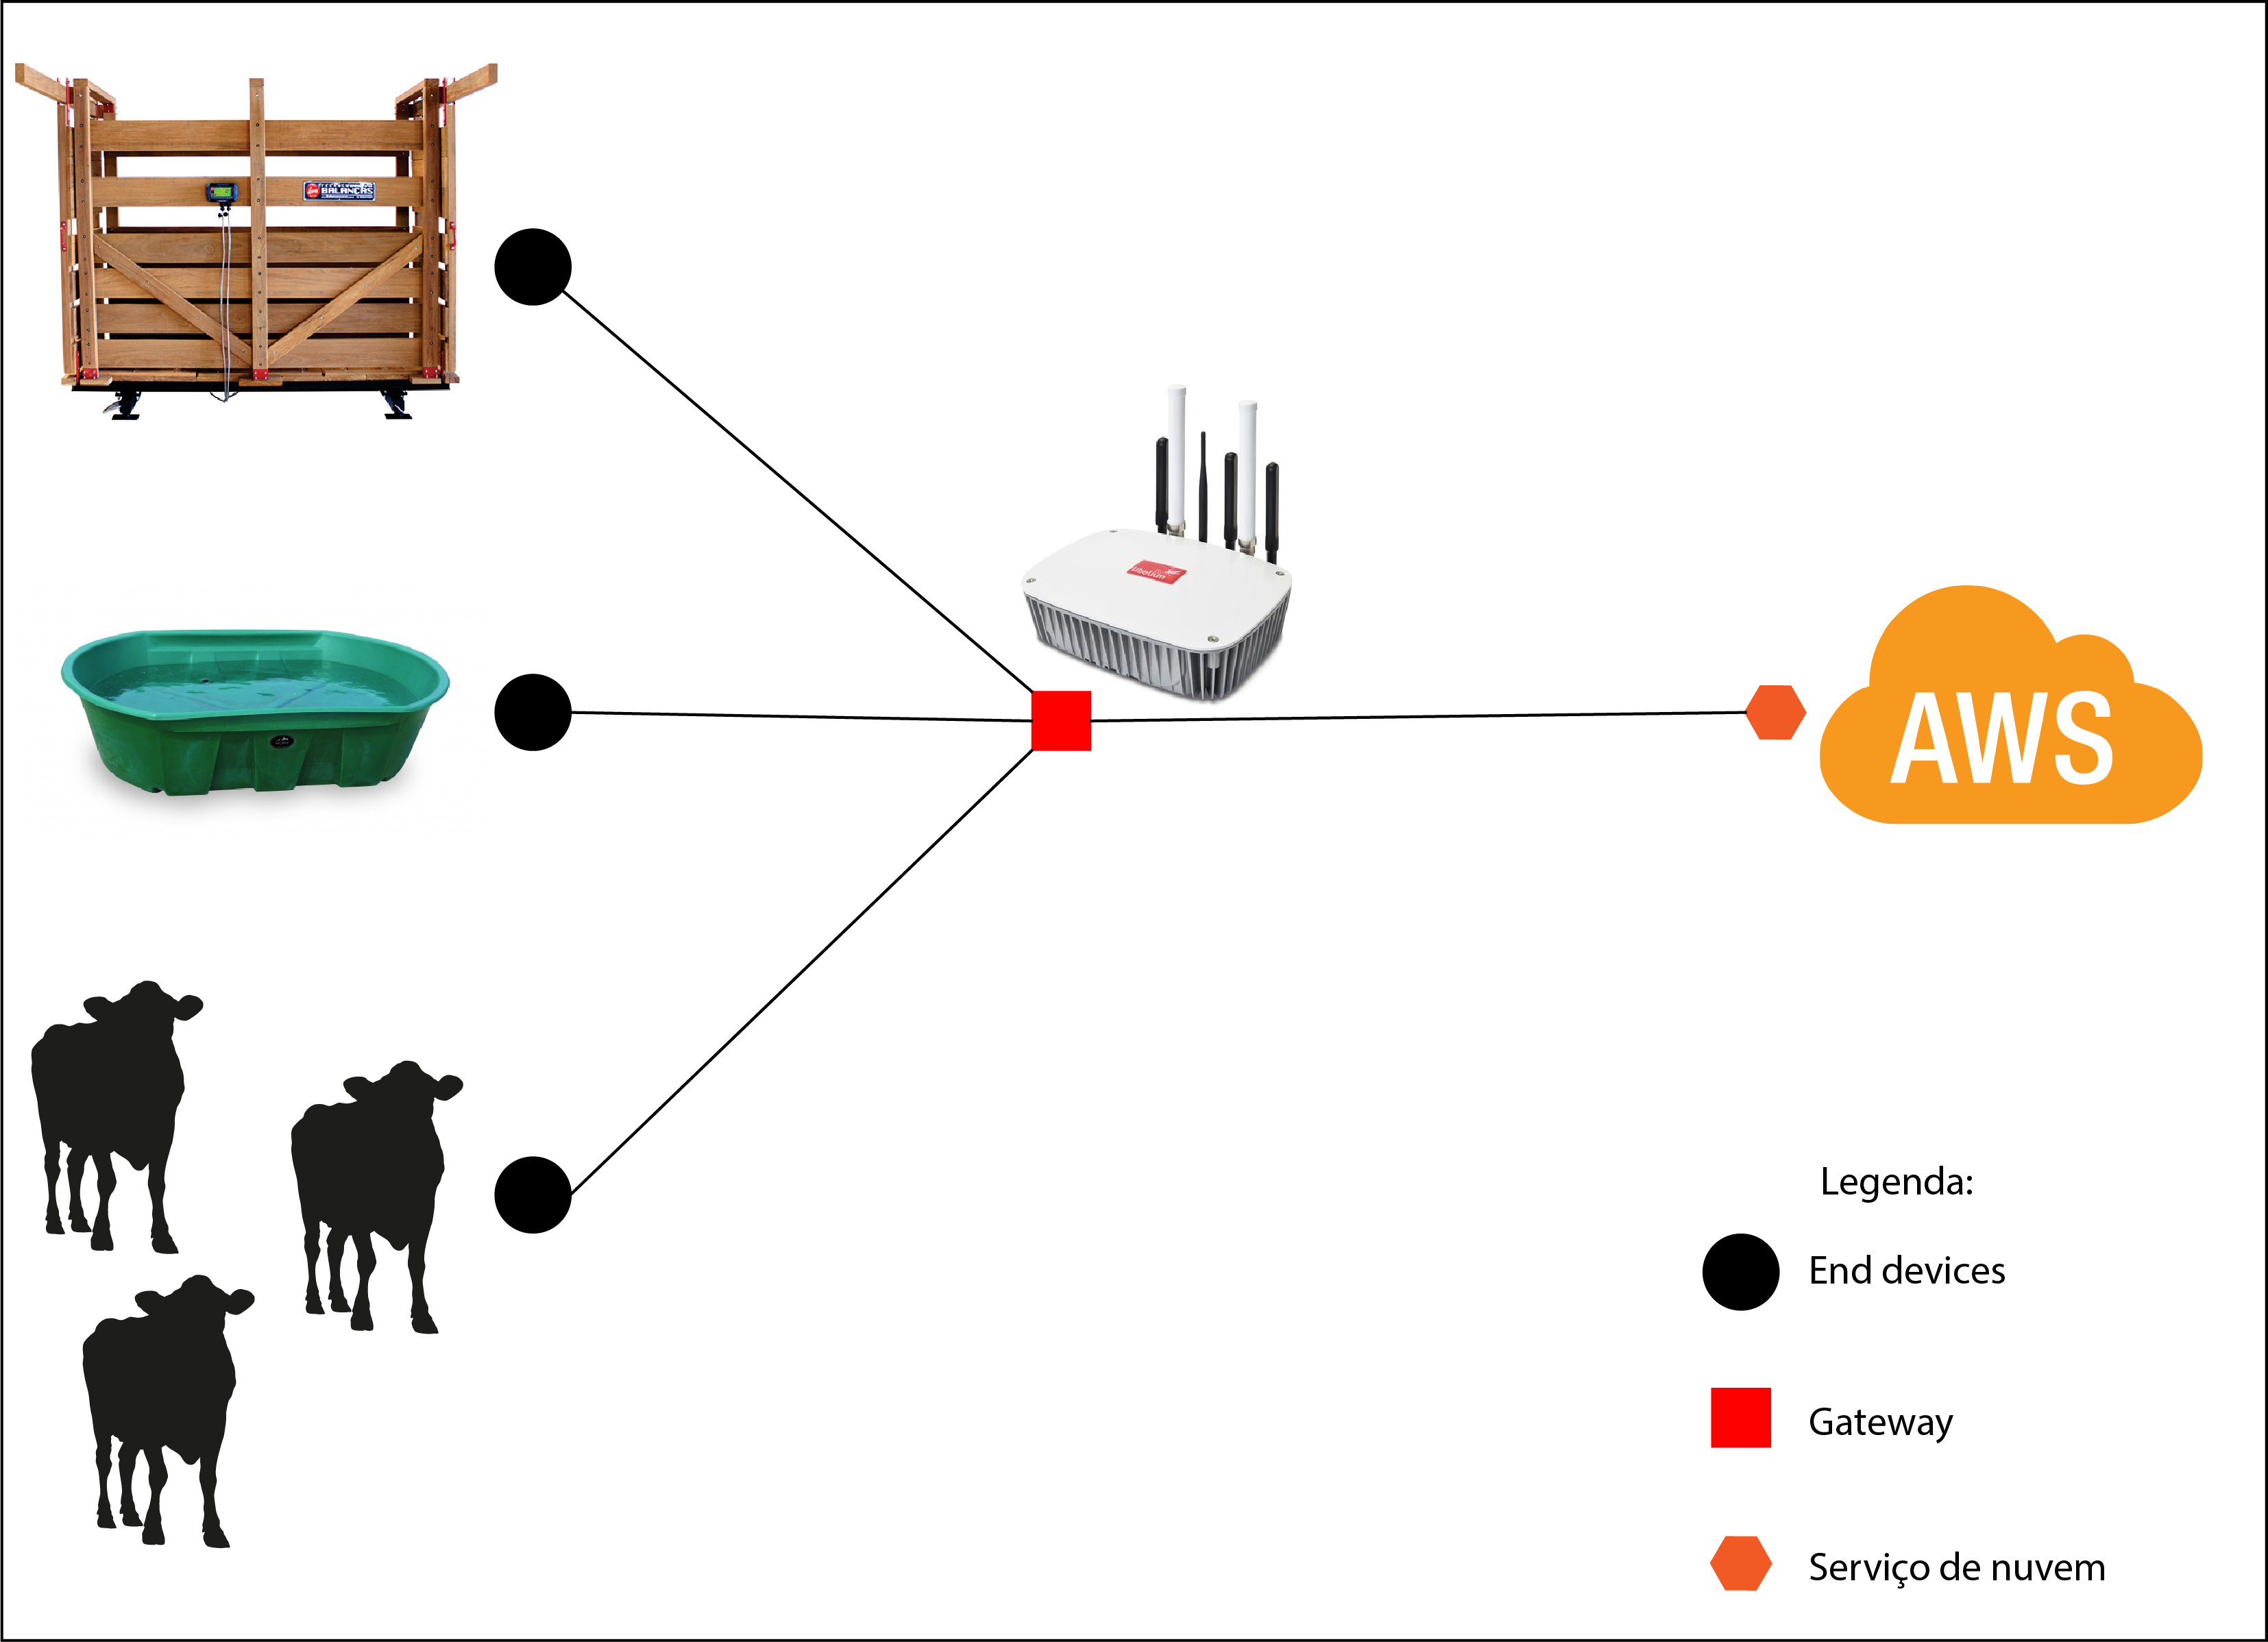
\includegraphics[width=1\textwidth]{big-picture.png}
    \legend{Fonte: Autor}
    \label{fig:bigpic}
\end{figure}

Definidos os parâmetros a serem monitorados, é interessante notar que alguns podem estar relacionados com o animal e outros podem estar relacionados com o ambiente. É esperado que diferentes dispostivos de borda estejam inseridos neste cenário.

Partindo desse princípio, nesta solução,  os coxos em que os animais bebem água são instrumentados com  um nó desenvolvido com diferentes tipos de sensores como objetivo de extrair dados relacionados com a qualidade da  água, tais como:  pH, oxigenação da água e temperatura. 
% A conectividade utilizará a tecnologia LoRaWAN, pois consegue transmitir informações a longo alcance e consome pouca energia.

% Para o monitoramento do gado, será prototipado um dispositivo de borda munido de sensor de temperatura, um módulo GPS, um giroscópio e acelerômetro. Esse nó também se comunicará utilizando a tecnologia LoRaWAN. O peso animal tem como propósito ser mensurado uma vez por mês. Entre pastos costuma-se ter um corredor para poder dirigir o gado para outros pastos em trocas destes. A instalação de uma balança neste corredor facilita a colheita da pesagem. Esta balança será ligada a um nó de transmissão, que transmitirá as medições também utilizando LoRaWAN. 

O gado é monitorado utilizando um dispositivo de borda contendo sensor de temperatura, um módulo GPS, um giroscópio e acelerômetro.

O peso animal tem como propósito ser mensurado uma vez por mês. Entre pastos costuma-se ter um corredor para poder dirigir o gado para outros pastos. A instalação de uma balança no corredor permite a colheita da pesagem. Esta balança éligada a um nó de transmissão, que transmitirá as medições para um \textit{gateway}.

Como mencionado no capítulo 2, a infraestrutura IoT  para o MannaWare poderia estar organizada como a seguir: três nós de borda, sendo um deles o coletor de informações da água, um nó sensor embutido no gado e o outro instalado na balança, sendo estes representados pelos círculos preenchidos de preto na figura \ref{fig:bigpic}. Esses dispositivos enviarão informações para um \textit{Gateway}, representado pelo quadrado vermelho da figura \ref{fig:bigpic}, podendo ser um protótipo com \textit{Raspberry Pi}, como citado no capítulo 2, subseção \ref{gateways}, ou um comercial como Meshlium Extreme. Caso a distância de algum desses dispositivos de borda exceda o limite de transmissão até o \textit{gateway}, será necessário o desenvolvimento de nós retransmissores.

Ao se tratar de um ambiente rural, é interessante utilizar rádios LoRa para a transmissão de informações entre dispositivos. Devido ao fato de até mesmo pequenas propriedades rurais possuírem como barreira as grandes distancias entre áreas e variáveis de interesse de monitoramento, como visto no capítulo \ref{cap2} na subseção \ref{lorawan} a tecnologia LoRa é uma solução para comunicação de longo alcance, prezando pelo baixo consumo de energia. Então é interessante que o  \textit{gateway} receba os pacotes de informações dos dispositivos de borda através de um módulo de rádio LoRa, e utilizando a API de acesso de algum serviço de nuvem, e armazene os dados recebidos nesta plataforma, representada pelo hexágono laranja da figura \ref{fig:bigpic} (como ilustração é apresentado o serviço da AWS). Com os dados armazenados em uma plataforma IoT em nuvem, uma aplicação, mobile ou web, pode ser desenvolvida para o acesso e manipulação desses dados pelos interessados: pecuaristas, agricultores, veterinários ou até mesmo 

% do serviço de nuvem AWS, armazenará os dados recebidos nesta plataforma, representada pelo hexágono laranja da figura \ref{fig:bigpic}. Com os dados armazenados em uma plataforma Internet das Coisas em \textit{cloud}, uma aplicação, mobile ou web, pode ser desenvolvida para o acesso e manipulação desses dados pelos interessados: pecuaristas, agricultores, veterinários ou até mesmo pesquisadores.

Esta solução consegue cobrir a infraestrutura definida do paradigma \textit{Internet of Things}, instrumentando um ambiente com diferentes tipos de sensores, que se comunicam a um \textit{gateway} ou até mesmo a outros dispositivos de borda, e que tem seus dados persistidos em uma plataforma em nuvem. Além de permitir a expansão da solução, podendo ser inseridos mais nós de borda coletando informações diferentes do ambiente, que tirará proveito da infraestrutura IoT presente no ambiente.  

% \section{Resumo}
% Este capítulo apresentou variáveis a serem monitoradas para auxiliar na criação de gado de engorda no ambiente rural. Explicou a importância de se monitorar cada uma dessas variáveis, bem como apresentou sugestões de como realizar esse monitoramento utilizando a infraestrutura da Internet das Coisas.

\setcounter{section}{0}
\chapter*[Capítulo 4]{Capítulo 4} \label{capitulo4}
\addcontentsline{toc}{chapter}{Capítulo 4}

% Após apresentar uma possível solução utilizando o paradigma da Internet das Coisas para uma aplicação que monitora o ambiente rural como um todo focado na criação do gado de engorda, este capítulo descreverá a implementação realizada com finalidade de cumprimento do trabalho de conclusão de curso, abordando as decisões de materiais a utilizados, bem como as variáveis escolhidas pa...

% O capítulo 3 propõe uma estrutura de aplicação para o monitoramento de um ambiente rural com foco no gado de engorda. Lá são levantas as variáveis de interesse a serem monitoradas, bem como uma sugestão de abordagem a se utilizar para esse objetivo. Este capítulo descreverá a aplicação desenvolvida com base no modelo proposto no capítulo anterior, justificando as variáveis de monitoramento escolhidas para o desenvolvimento deste trabalho. Também serão justificadas as escolhas de tecnologia.

Este capítulo trata do desenvolvimento da aplicação definida como estudo de caso. A solução proposta envolve a definição de parâmetros e o uso de tecnologia. Os materiais e métodos bem como as decisões de projeto estão estão descritas ao longo do texto.

\section{Parâmetros de monitoramento da prova de conceitos}

Dentre as variáveis apresentadas na Seção \ref{variaveis} do Capítulo \ref{capitulo3}, foram escolhidas as de qualidade da água e geolocalização do animal para a prova de conceito e estudo de caso. Essa escolha foi feita para se ter dois dispositivos de borda com propostas diferentes presentes na rede. Outro motivo é o de justificar o monitoramento do ambiente rural como um todo, e não somente o animal inserido nele. 

Um outro fator para essa escolha foi a disponibilidade de hardware no laboratório Manna/UEM para a prototipação. Restrições de e orçamento também impediram a aquisição e utilização de sensores e hardwares necessários para o desenvolvimento da solução proposta.

\section{Materiais e métodos}
Considerando os requisitos funcionais estabelecidos a partir da escolha das variáveis a serem monitoradas, os elementos de hardware foram definidos como parte da solução. Existem alguns modelos disponíveis comercialmente. Contudo, a burocracia para compra e os valores impediram a aquisição de plataformas. Coube, então, utilizar os nós disponíveis no laboratório Manna/UEM, sendo eles:

% foram escolhidas as tecnologias para o desenvolvimento da aplicação. Utilizando a infraestrutura IoT definida no capitulo \ref{cap2} seção \ref{infraIoT}, escolheu-se os hardwares para compor os dois modelos de nós de borda e o gateway. Como justificado no capítulo \ref{capitulo3} seção \ref{modeloaplicacao}, a comunicação entre os dispositivos de borda e o \textit{gateway} será feita utilizando LoRa.

Para desenvolver os dispositivos sensores e o \textit{gateway} foram escolhidos os seguintes hardwares:

\begin{itemize}
\item Módulos de radio RFM95W: é um transceptor de radio (figura \ref{fig:rfm95w}) que utiliza da tecnologia LoRa e é fabricado pela HopeRF que entrega até +20dBm de potência. O módulo RFM95W foi escolhido pois possui um distribuidor local deste circuito. Rádios LoRa não são comumente encontrados para a comercialização no Brasil, enquanto para a importação se acha diversos dispositivos embutidos com módulos de radio LoRa e até mesmo com sensores e microcontroladores já integrados. Assim, optou-se por comprar duas unidades do rádio RFM95W.

\begin{figure}[ht]
    \centering
    \caption{\textit{Módulo de radio RFM95W}}
    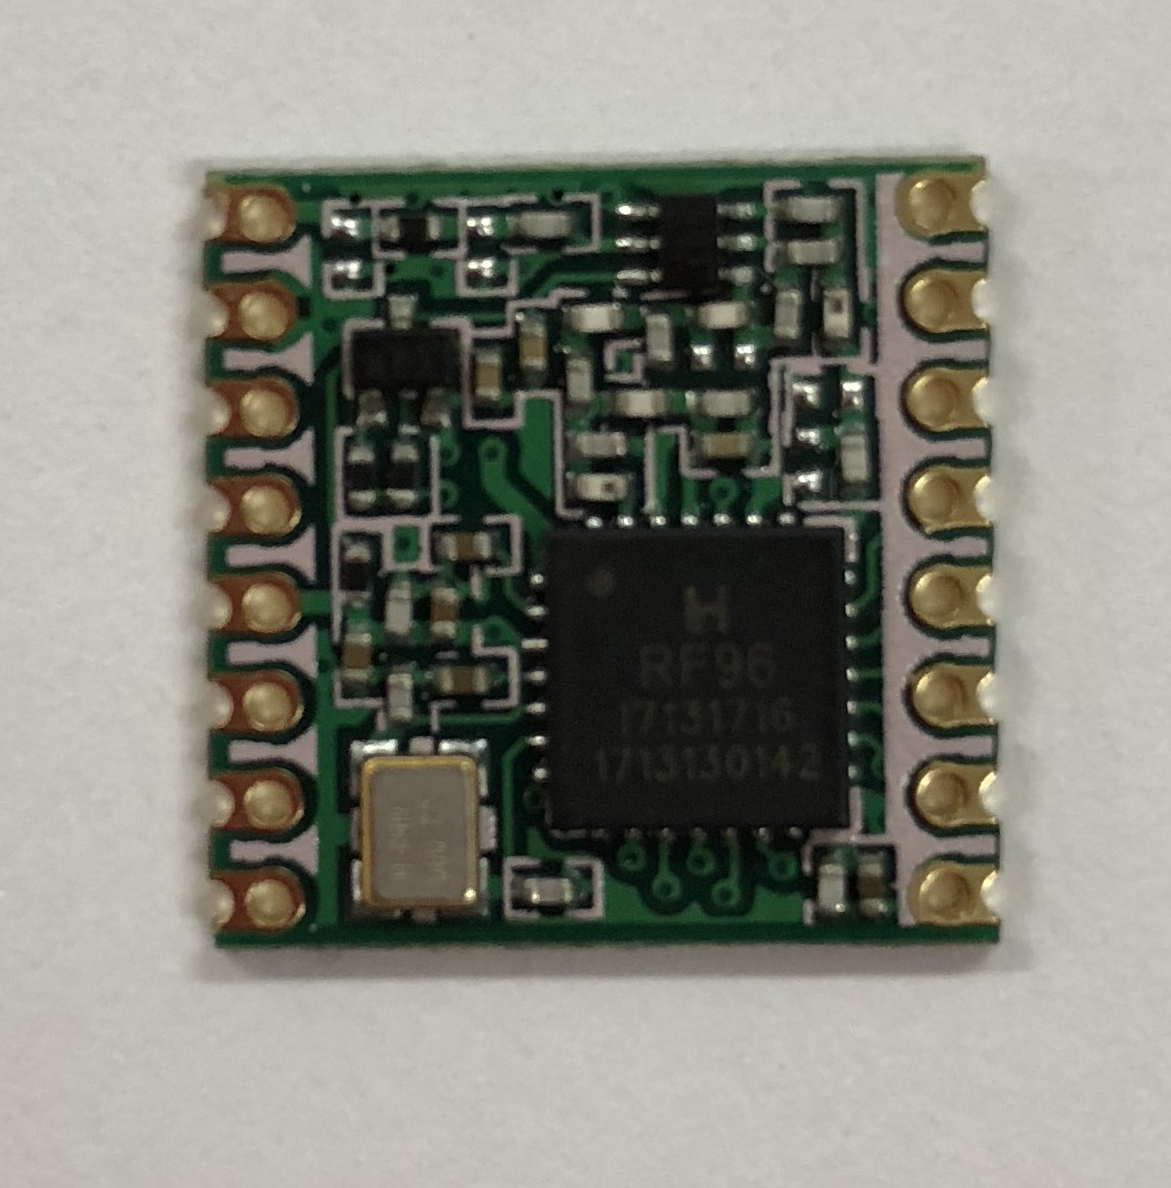
\includegraphics[width=0.5\textwidth]{rfm95w.png}
    \legend{Fonte: Autor}
    \label{fig:rfm95w}
\end{figure}

\item Microcontrolador Heltec ESP32 LoRa: é um microcontrolador produzido pela empresa Heltec semelhante a um Arduino Nano que contém embutido um módulo WiFi e um módulo LoRa SX1278 produzido pela empresa Semtech (figura \ref{fig:esp32}). O circuito conta com um \textit{display} OLED de 0,96 polegadas. Com a chagada do nó em tempo de realizar testes na rede proposta para esse trabalho, decidiu-se por incluí-lo no desenvolvimento como forma de comparação entre um módulo rádio RFM95W soldado manualmente de forma amadora e uma solução pronta no mercado. O circuito produzido pela Semtech tem configuração semelhante ao da HopeRF, podendo entregar também até entrega +20dBm de potência.

\begin{figure}[ht]
    \centering
    \caption{\textit{Dispositivo ESP32 contendo um módulo de rádio LoRa}}
    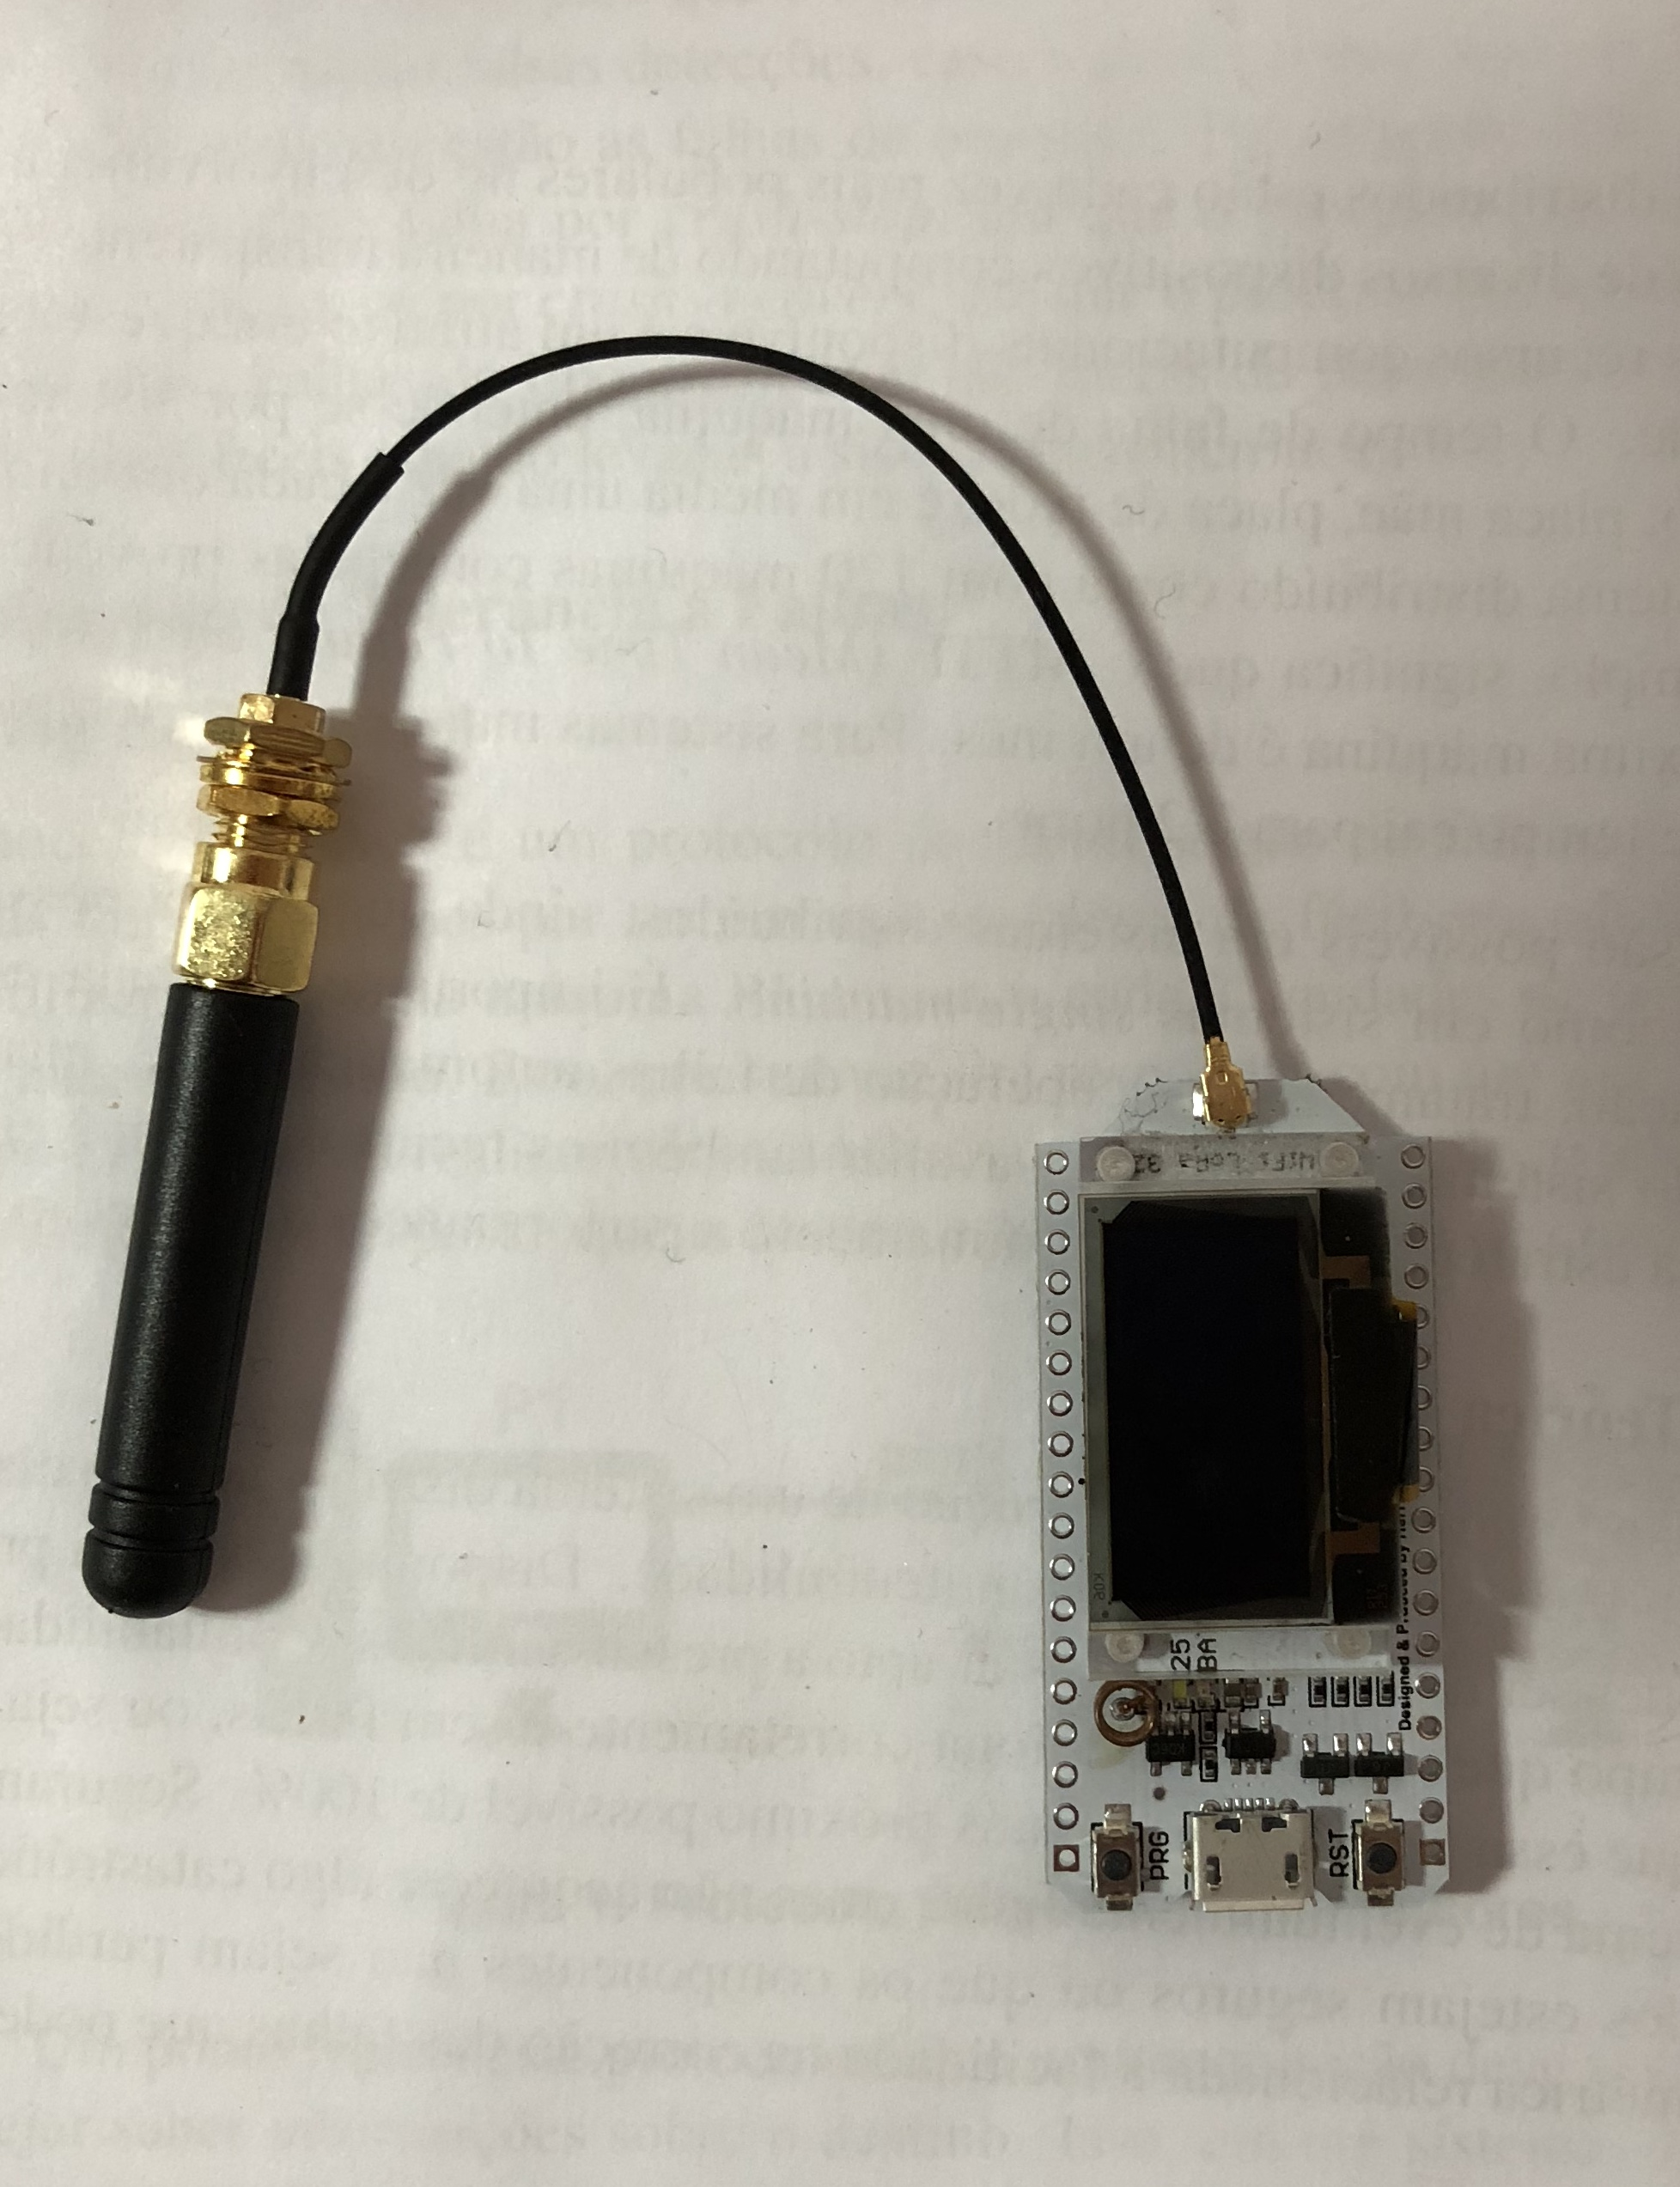
\includegraphics[width=0.5\textwidth]{esp32.jpg}
    \legend{Fonte: Autor}
    \label{fig:esp32}
\end{figure}

\item Sensor de temperatura DS18B20: é um sensor digital que consegue medir a temperatura de -55 graus Celsius até +125 graus Celsius, com uma acurácia de mais ou menos 0,5 graus entre as temperaturas de -10 a +85. Este sensor possui uma versão a prova da água, o que seria melhor para o proposito da aplicação tendo em vista que a temperatura seria a variável de qualidade da água escolhida para exemplificar a solução. Devido a indisponibilidade desse tipo de sensor, foi utilizado o modelo da figura \ref{fig:DS18B20} com o propósito de simular a colheita do parâmetro de temperatura da água.

\begin{figure}[ht]
    \centering
    \caption{Sensor de temperatura DS18B20}
    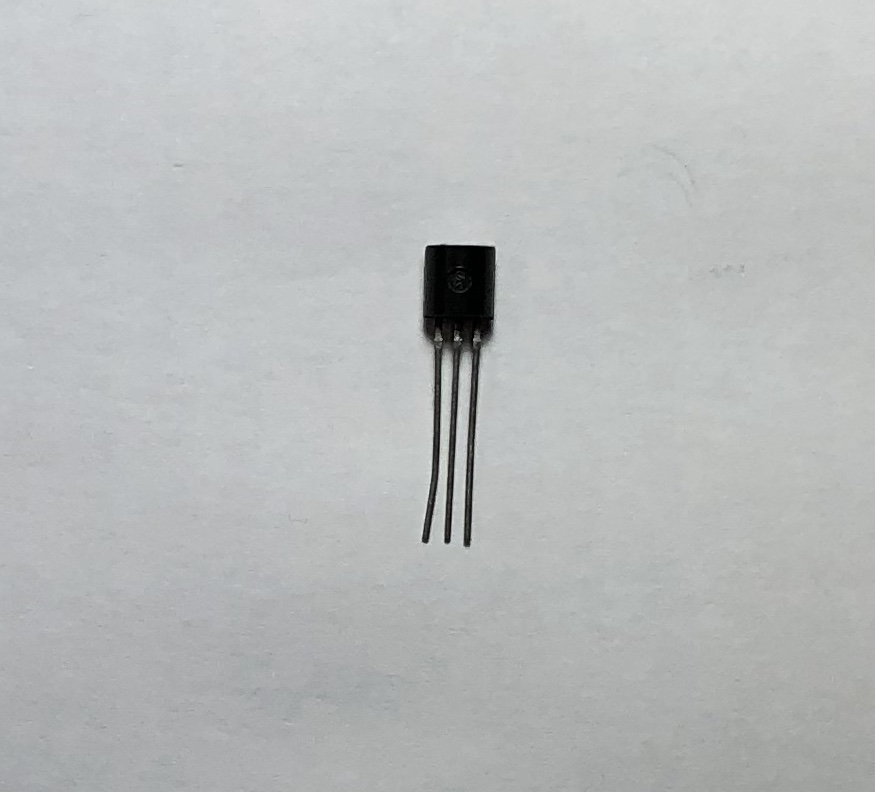
\includegraphics[width=0.25\textwidth]{ds18b20.jpg}
    \legend{Fonte: Autor}
    \label{fig:DS18B20}
\end{figure}

\item Módulo GPS v1r3 TinySine: é um \textit{shield} para Arduino Uno e similares produzido pela empresa TinySine. Este \textit{shield} é um \textit{logger} de GPS, contendo uma entrada para cartão SD, suportando então o armazenamento de dados localmente. Como o propósito da aplicação é utilizar da estrutura da Internet das Coisas, essa placa serviu somente para a coleta dos dados de GPS, e não o armazenamento local. Este modelo de GPS foi escolhido por existir vários exemplares disponíveis no laboratório de pesquisa Manna/UEM.

\begin{figure}[ht]
    \centering
    \caption{\textit{Shield GPS v1r3 TinySine}}
    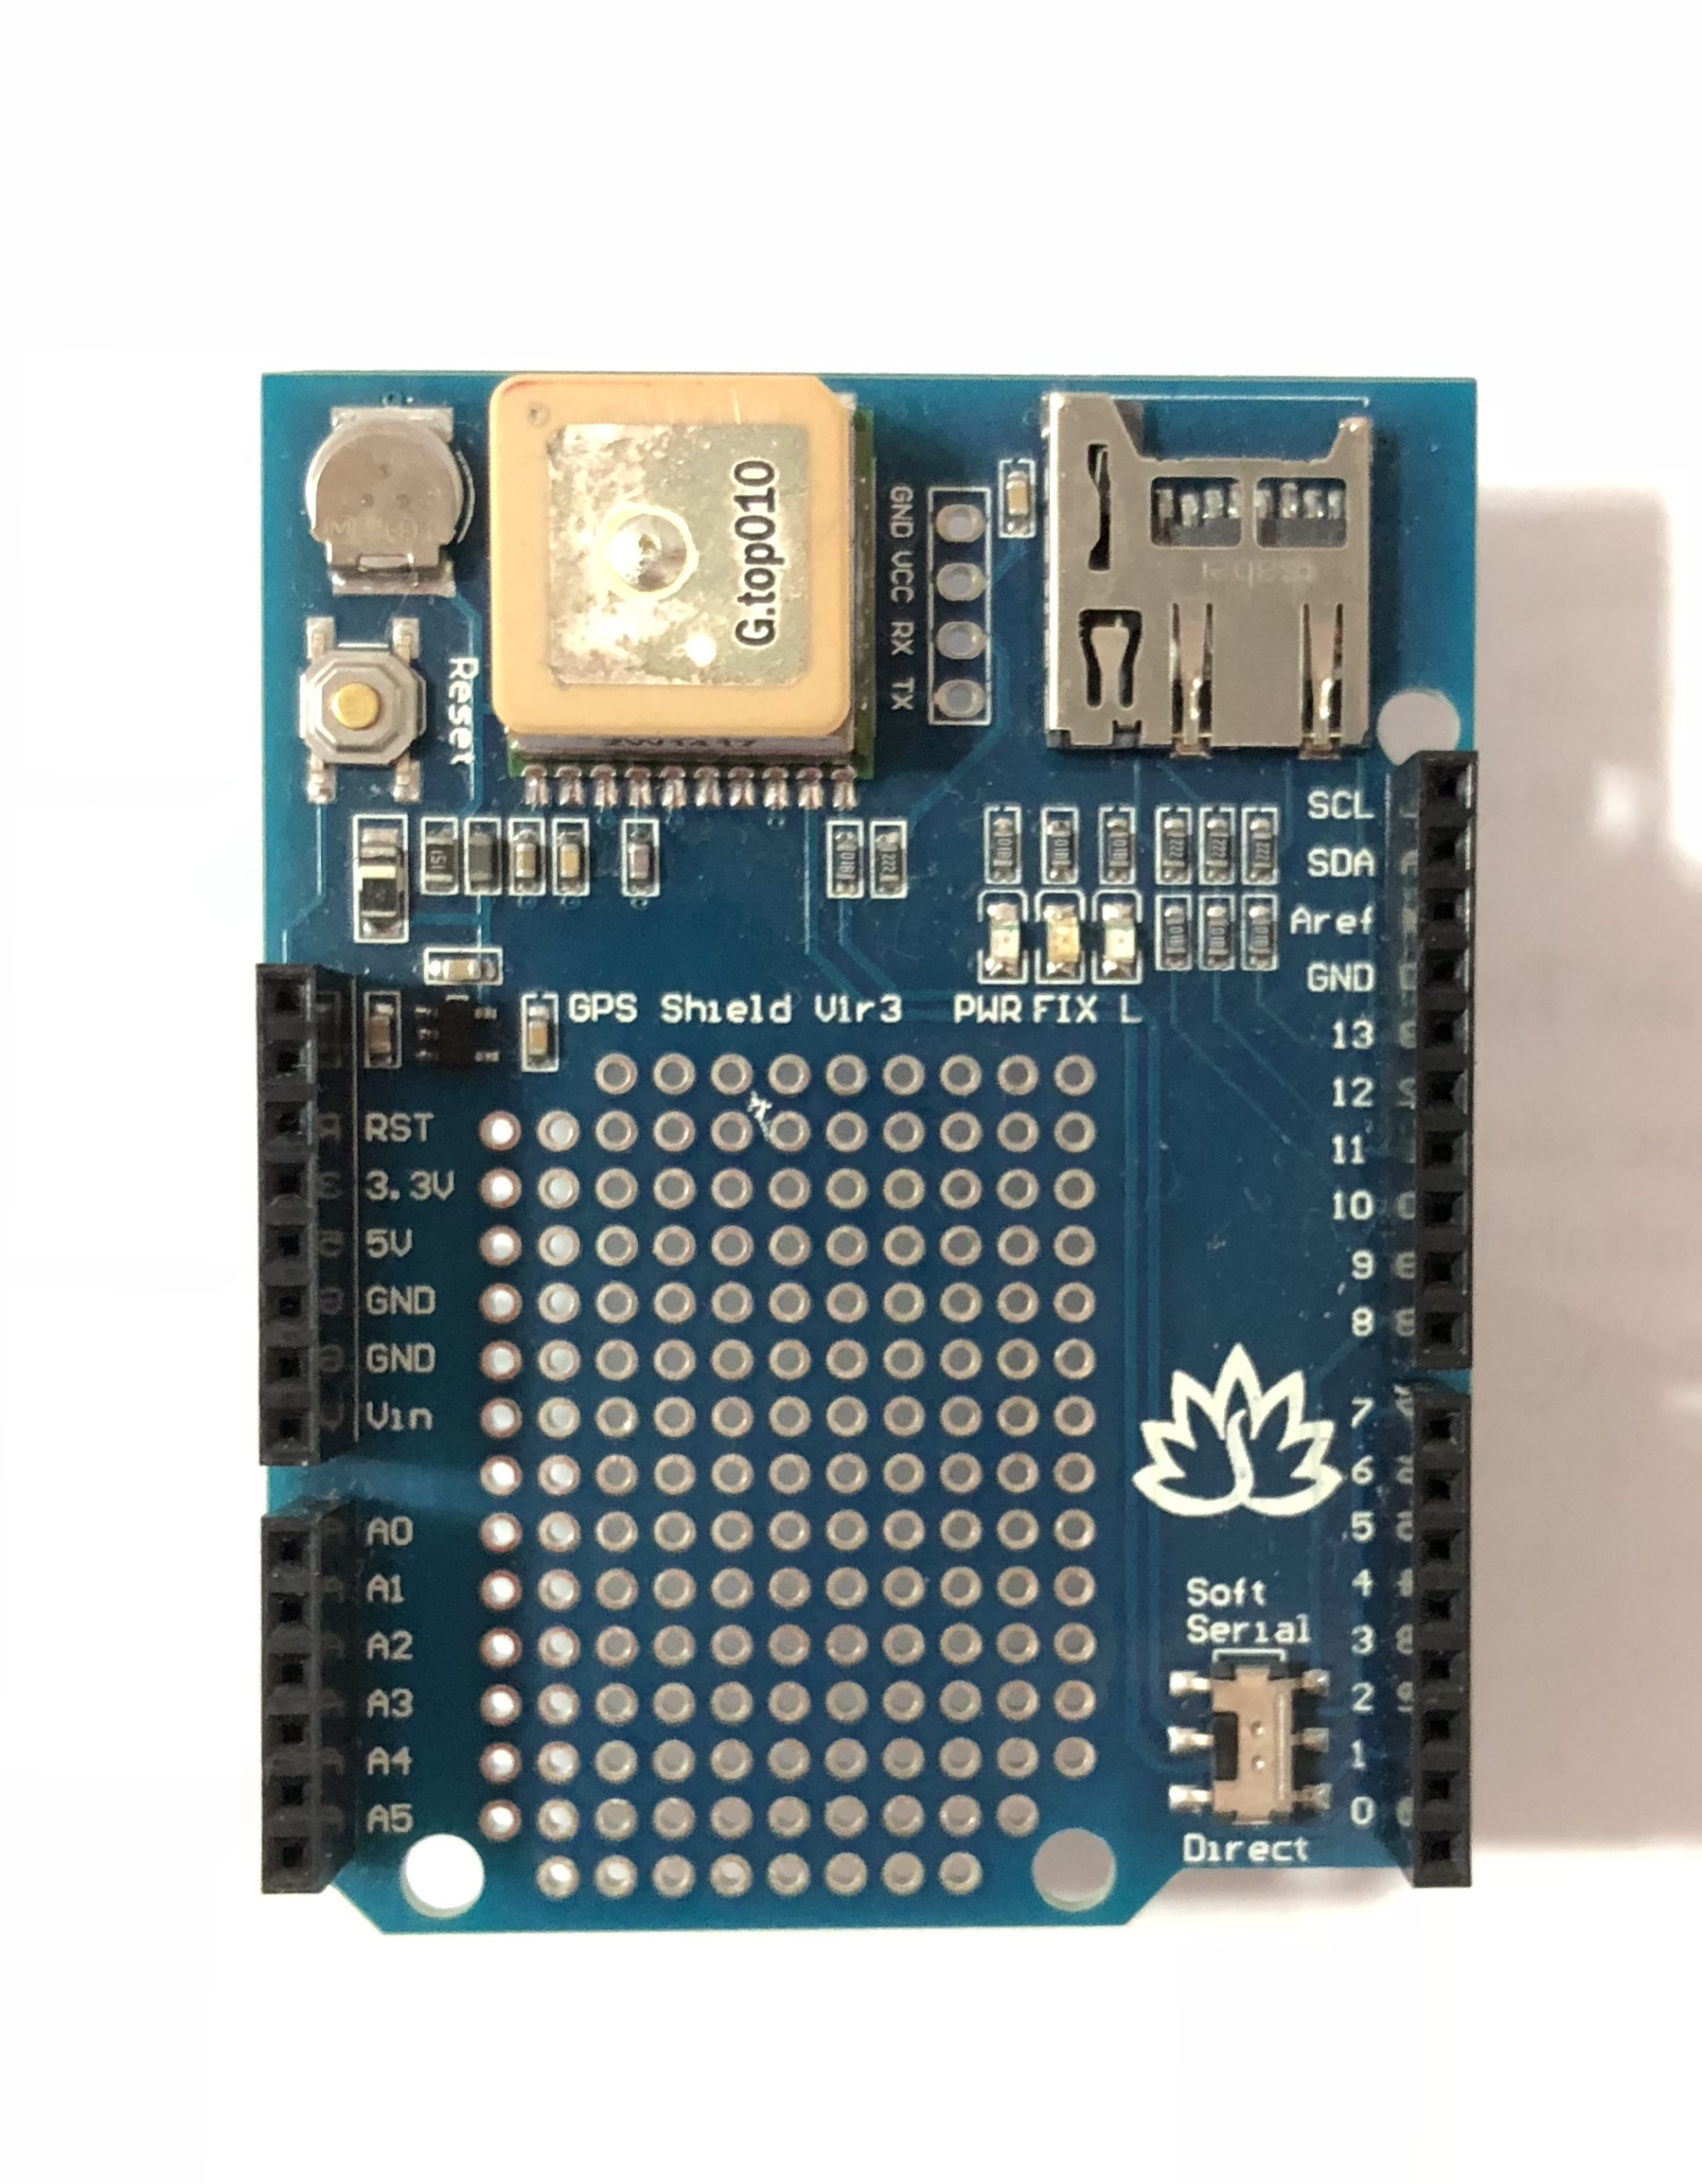
\includegraphics[width=0.5\textwidth]{tinysine.jpg}
    \legend{Fonte: Autor}
    \label{fig:tinysine}
\end{figure}

\item Raspberry pi 3 \textit{model} B: um microcomputador, figura \ref{fig:rpi}, que foi escolhido como \textit{gateway} devido a suas dimensões pequenas, o que favorece positivamente o manuseio e portabilidade. Conta com 1GB de memória RAM, e tem suporte de um sistema operacional baseado no Debian, o Raspbian, permitindo o uso de ferramentas e execução de códigos e \textit{scripts}. Possui portas de entrada e saída de proposito geral (GPIO) permitindo a ligação entre ele e um módulo de rádio LoRa. Outro fator importante para a escolha desse material para a confecção do \textit{gateway} é a possibilidade de conexão cabeada ou sem fio com a internet, tornando o microcomputador versátil e de propósito geral, por isso sendo um computador comum nas prototipações.
\end{itemize}

\begin{figure}[ht]
    \centering
    \caption{\textit{Raspberry Pi model 3 B}}
    \legend{Fonte: Autor}
    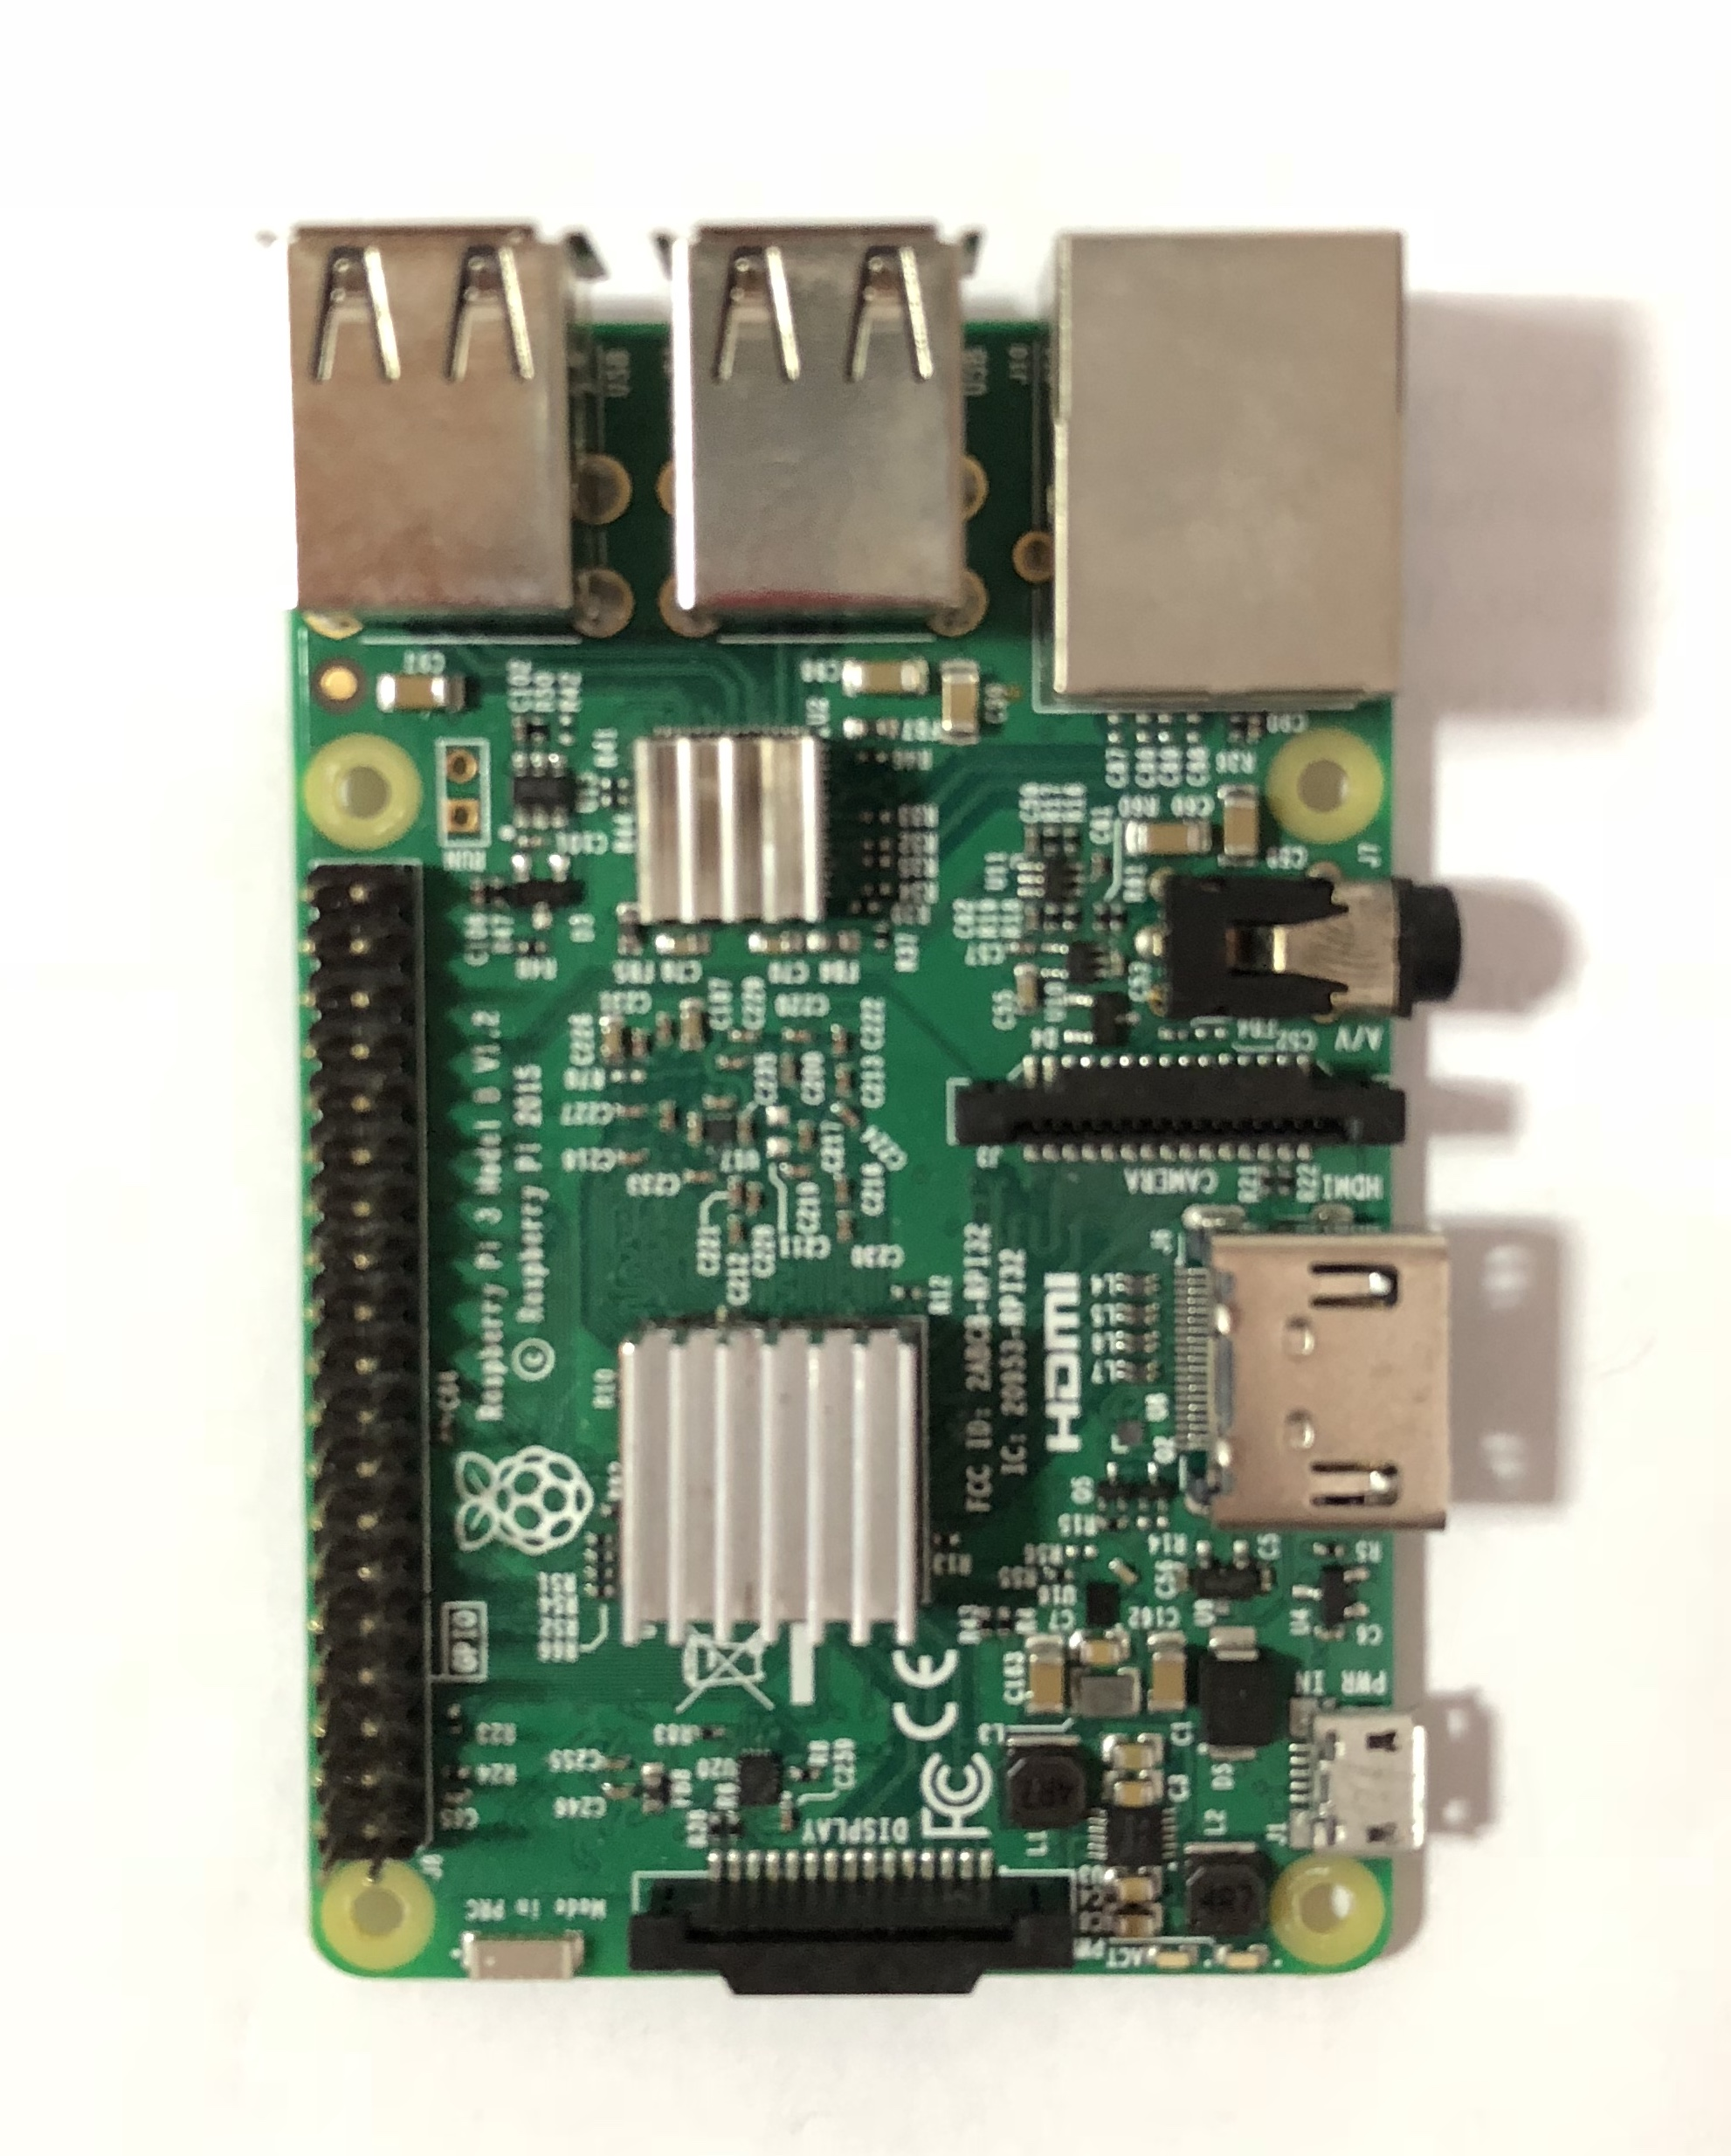
\includegraphics[width=0.5\textwidth]{rpi.jpg}
    \label{fig:rpi}
\end{figure}


\section{Prototipando a solução com a IoT}

A prototipação de IoT em ambiente rural, considerando a aplicação de, em particular, gado de engorda, proposta como estudo de caso, bem como os materiais disponíveis, tem a seguinte composição de infraestrutura: dois nós de borda, um \textit{gateway} para receber a informação desses nós e armazenar em uma plataforma de nuvem IoT. 

O serviço de comunicação é baseado na tecnologia LoRa. A aplicação proposta também tem o objetivo de realizar um estudo inicial sobre o uso desta tecnologia em ambientes rurais. Para a definição da melhor configuração desta tecnologia, testes foram realizados como descritos na próxima seção.

\subsection{Teste de distância dos módulos de rádio LoRa}
Com o intuito de saber quais módulos de rádio LoRa disponíveis utilizar para cada propósito, realizou-se um teste de distância com o ESP32 e o RFM95W.  

Definiu-se que primeiramente um ESP32 ficaria fixado em um local atuando como um disparador de pacotes, enquanto um outro ESP32 seria deslocado em linha reta atuando como receptor de pacotes com propósito de observar até que distância ainda era possível receber informações do disparador. Em seguida, o disparador fixo seria substituído por um RFM95W ligado a um Arduino Uno, e o processo de deslocar o ESP32 atuando em modo de recepção se repetiria. O local escolhido para teste foi a Universidade Estadual de Maringá, na localidade de uma rua em linha reta, com presença de muitas árvores e algumas construções ao redor. Também a escolha foi feita por a maior parte deste percurso ser plano, possibilitando a comparação de recepção de sinal entre os dois módulos. O código dos disparadores para fins de teste enviavam um pacote com uma \textit{string} "Hello". 

Os resultados do teste podem ser conferidos na imagem \ref{fig:disttest}. O ponto envolvido por um quadrado se refere ao disparador de mensagens, que hora foi um ESP32, e hora foi um Arduino Uno com um RFM95W ligado a ele. O ponto envolto por um círculo se refere ao local em que foram recebidos os últimos pacotes enviados pelo ESP32, a 1 quilometro de distância entre os nós. O ponto envolto por um hexágono mostra o local em que foram recebidos os últimos pacotes enviados pelo RFM95W, a 1,11 quilometro de distância.

\begin{figure}[ht]
    \centering
    \caption{Teste de distância realizado com o Heltec ESP32 LoRa e o RFM95W na Universidade Estadual de Maringá}
    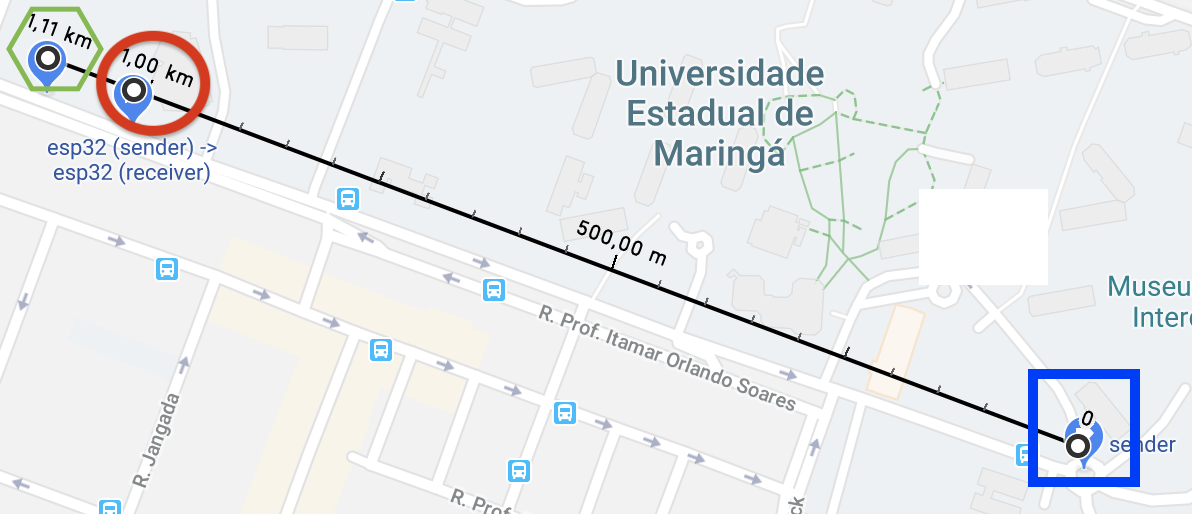
\includegraphics[width=1\textwidth]{distance_test.png}
    \legend{Fonte: Autor}
    \label{fig:disttest}
\end{figure}

Para a confecção do \textit{sender} RFM95W+Arduino, foi soldado manualmente de maneira artesanal fios de cobre nas entradas do módulo da HopeRF, por falta de prática com solda e indisponibilidade de serviços especializados na região. Este foi então conectado a uma \textit{protoboard}, e com \textit{jumper} ligado a uma antena conectada em um adaptador SMA. A ligação entre o Arduino Uno e o RFM95W pode ser conferida no anexo \ref{anexohardware}. Esta observação é feita devido ao fato de que, caso mal soldado e mal conectado o módulo de rádio está, e também dependendo da distância em que a antena se encontra ligada a ele, bem como a qualidade desta antena, são todos fatores que podem causar interferência no hardware e assim fazer com que a distância de comunicação diminua drasticamente do prometido. Mesmo sendo uma produção caseira não apresentando a qualidade de um nó feito com circuitos impressos e soldados por máquinas, a combinaçãpo RFM95W e Arduino conseguiram um alcance maior que o ESP32 na recepção de pacotes.

A partir desse resultado, foi decidido utilizar um RFM95W para compor o Gateway juntamente com o \textit{Raspberry Pi} e uma plataforma de nuvem. Uma aplicação  \textit{web} simples, MannaWare, foi desenvolvida para mostrar ao usuário final os dados coletados pelos dois nós de bordas da rede IoT. Nas próximas seções serão descrita a montagem de cada parte dessa infraestrutura, que terá como resultado a rede representada pela figura \ref{fig:bigpicprototipo}, que contém uma \textit{big picture} da aplicação, em que cada retângulo contem dentro de si os componentes de hardware, e o ultimo retângulo representa o protótipo do aplicativo web MannaWare. A combinação presente na representação da figura para a composição dos nós de borda e \textit{gateway} tomou como base o teste de distância descrito, e essas escolhas de montagem também serão melhores explicadas nas próximas subseções. Também será explicado o desenvolvimento do protótipo do aplicativo MannaWare.

\begin{figure}[ht]
    \centering   
    \caption{\textit{Big Picture} do protótipo proposto para o monitoramento do ambiente rural com foco em gado de engorda}
    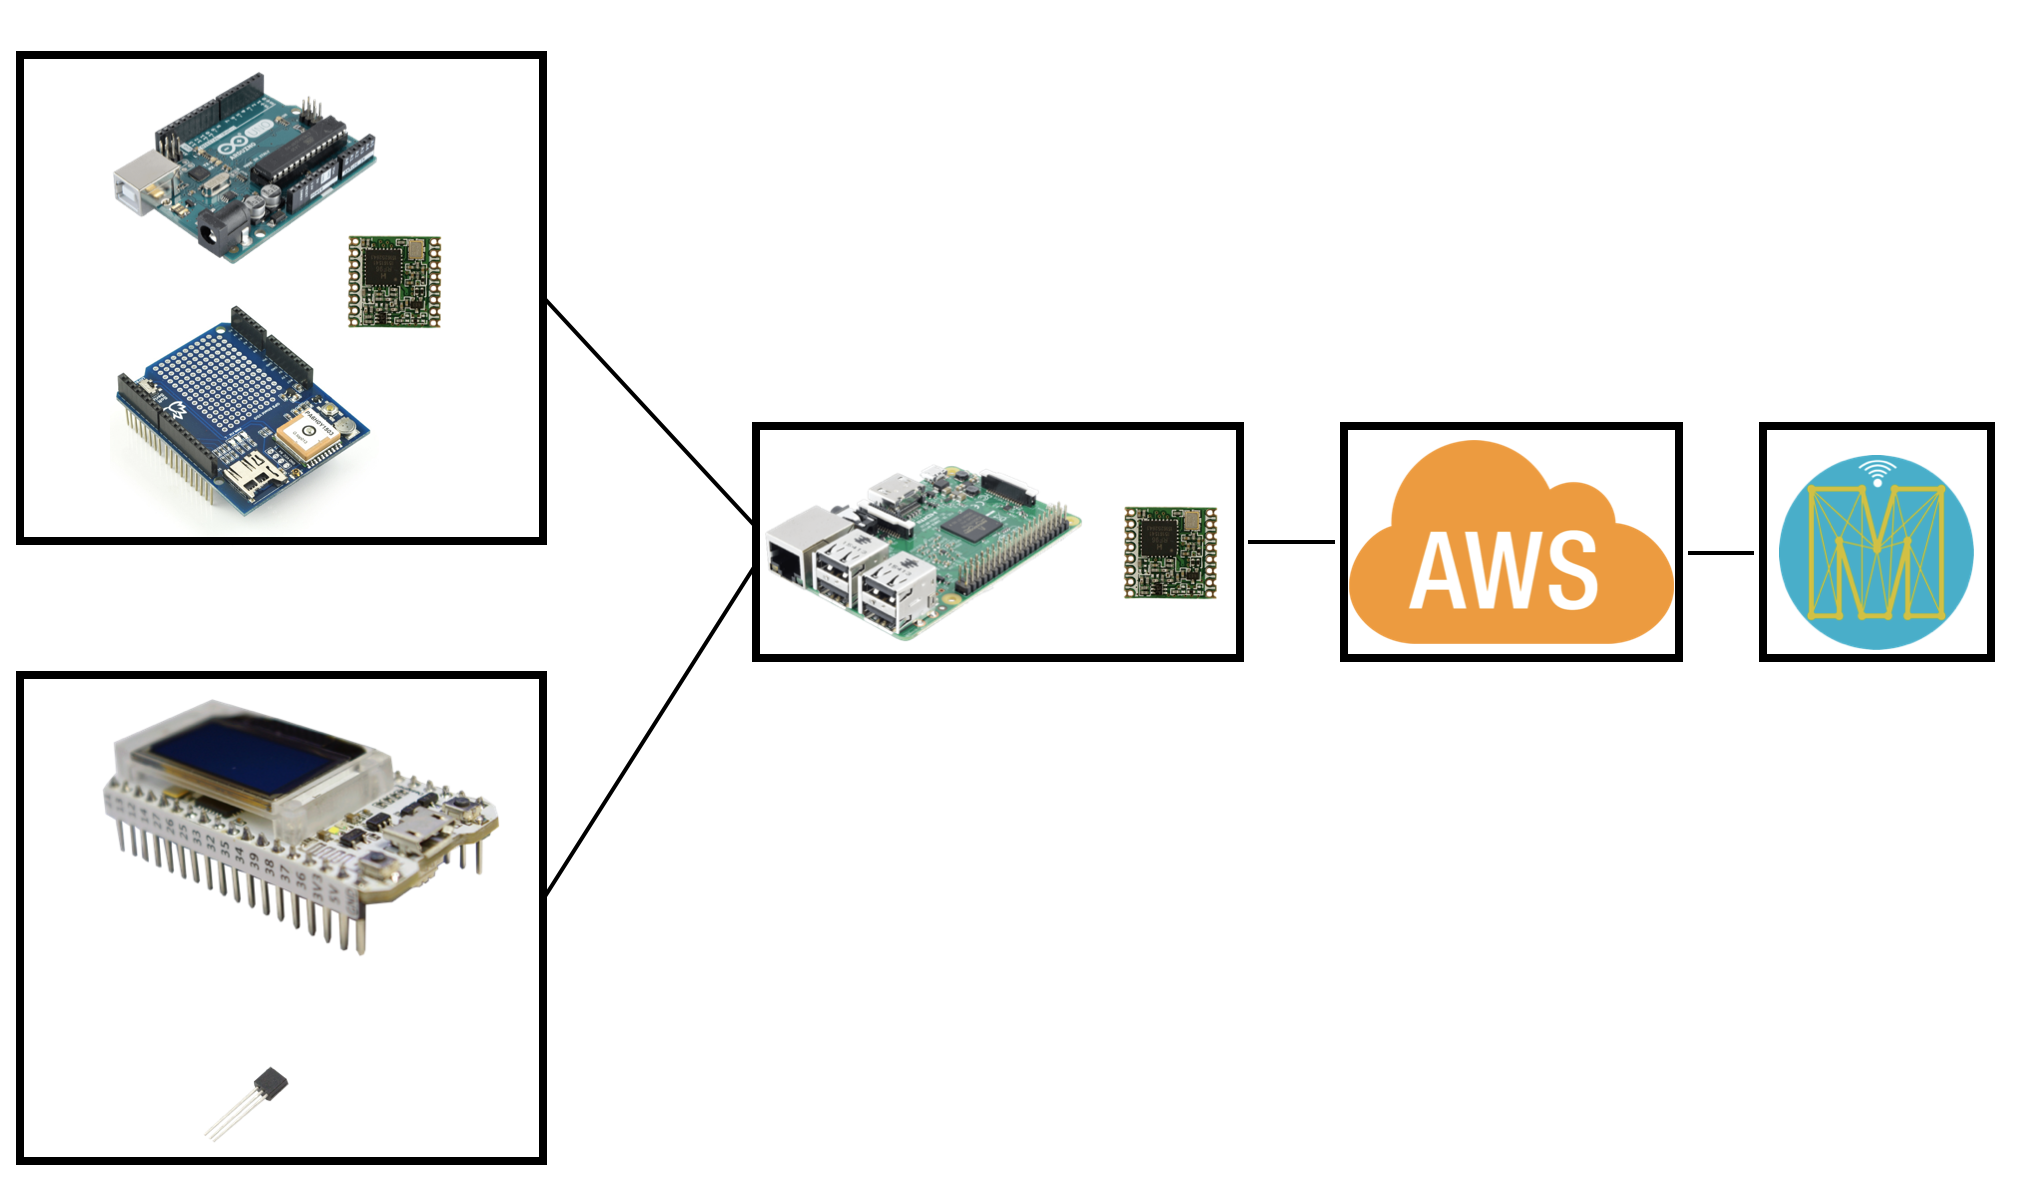
\includegraphics[width=1\textwidth]{bigpictureprototipomannaware.png}
    \legend{Fonte: Autor}
    \label{fig:bigpicprototipo}
\end{figure}

\subsection{Protótipo dos nós de borda}

Anteriormente foi definido os dois nós de borda, um responsável pelo monitoramento da variável de localização do gado através de um módulo GPS e o outro responsável pela medição de qualidade da água sendo representado por um nó de sensor de temperatura. Como apresentado na big picture (figura \ref{fig:bigpicprototipo}), o nó com o módulo GPS é composto por um Arduino Uno ligado ao \textit{shield TinySine v1r3} pelo fato deste componente ser desenhado para encaixar em Unos e similares. O módulo rádio escolhido para este \textit{device} foi o RFM95W por ser mais simples de se acoplar neste hardware. A imagem com a ligação de fios desse nó de borda encontra-se no anexo \ref{anexohardware}. A figura \ref{fig:gps1} mostra o resultado prático utilizado no protótipo deste trabalho.

\begin{figure}[ht]
    \centering
    \caption{Dispositivo de borda para coleta do parâmetro de geolocalização}
    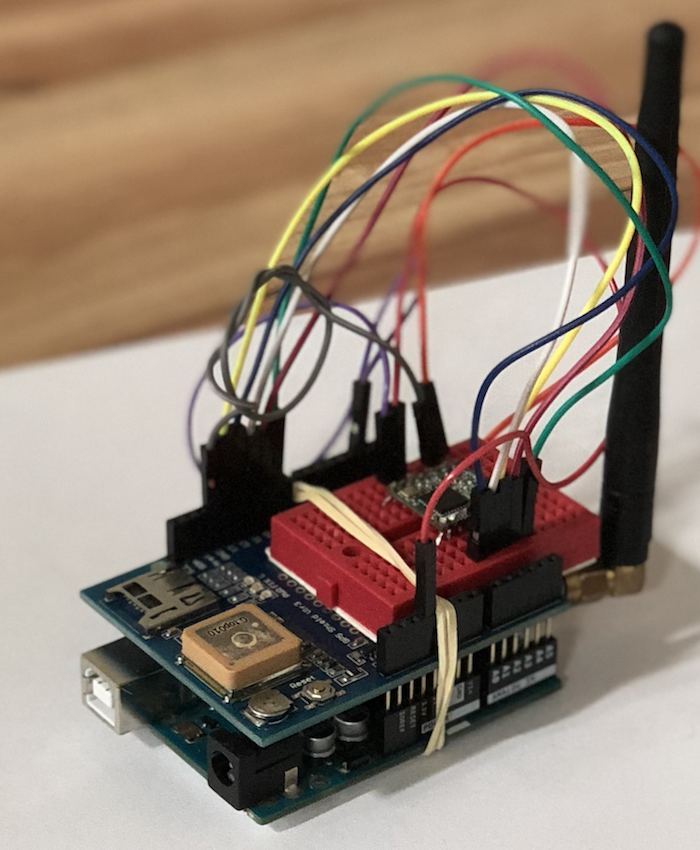
\includegraphics[width=0.5\textwidth]{gps1.png}
    \legend{Fonte: Autor}
    \label{fig:gps1}
\end{figure}

O nó de borda com o sensor de temperatura é composto pelo sensor DS18B20 ligado ao Heltec ESP32 LoRa. O resultado da montagem na prática pode ser observado na figura \ref{fig:temp1}. A imagem com a ligação detalhada dos fios pode ser encontrada no anexo \ref{anexohardware}. 

\begin{figure}[ht]
    \centering
    \caption{Dispositivo de borda coletor de temperatura utilizando o módulo Heltec ESP32 LoRa e o sensor de temperatura digital DS18B20}
    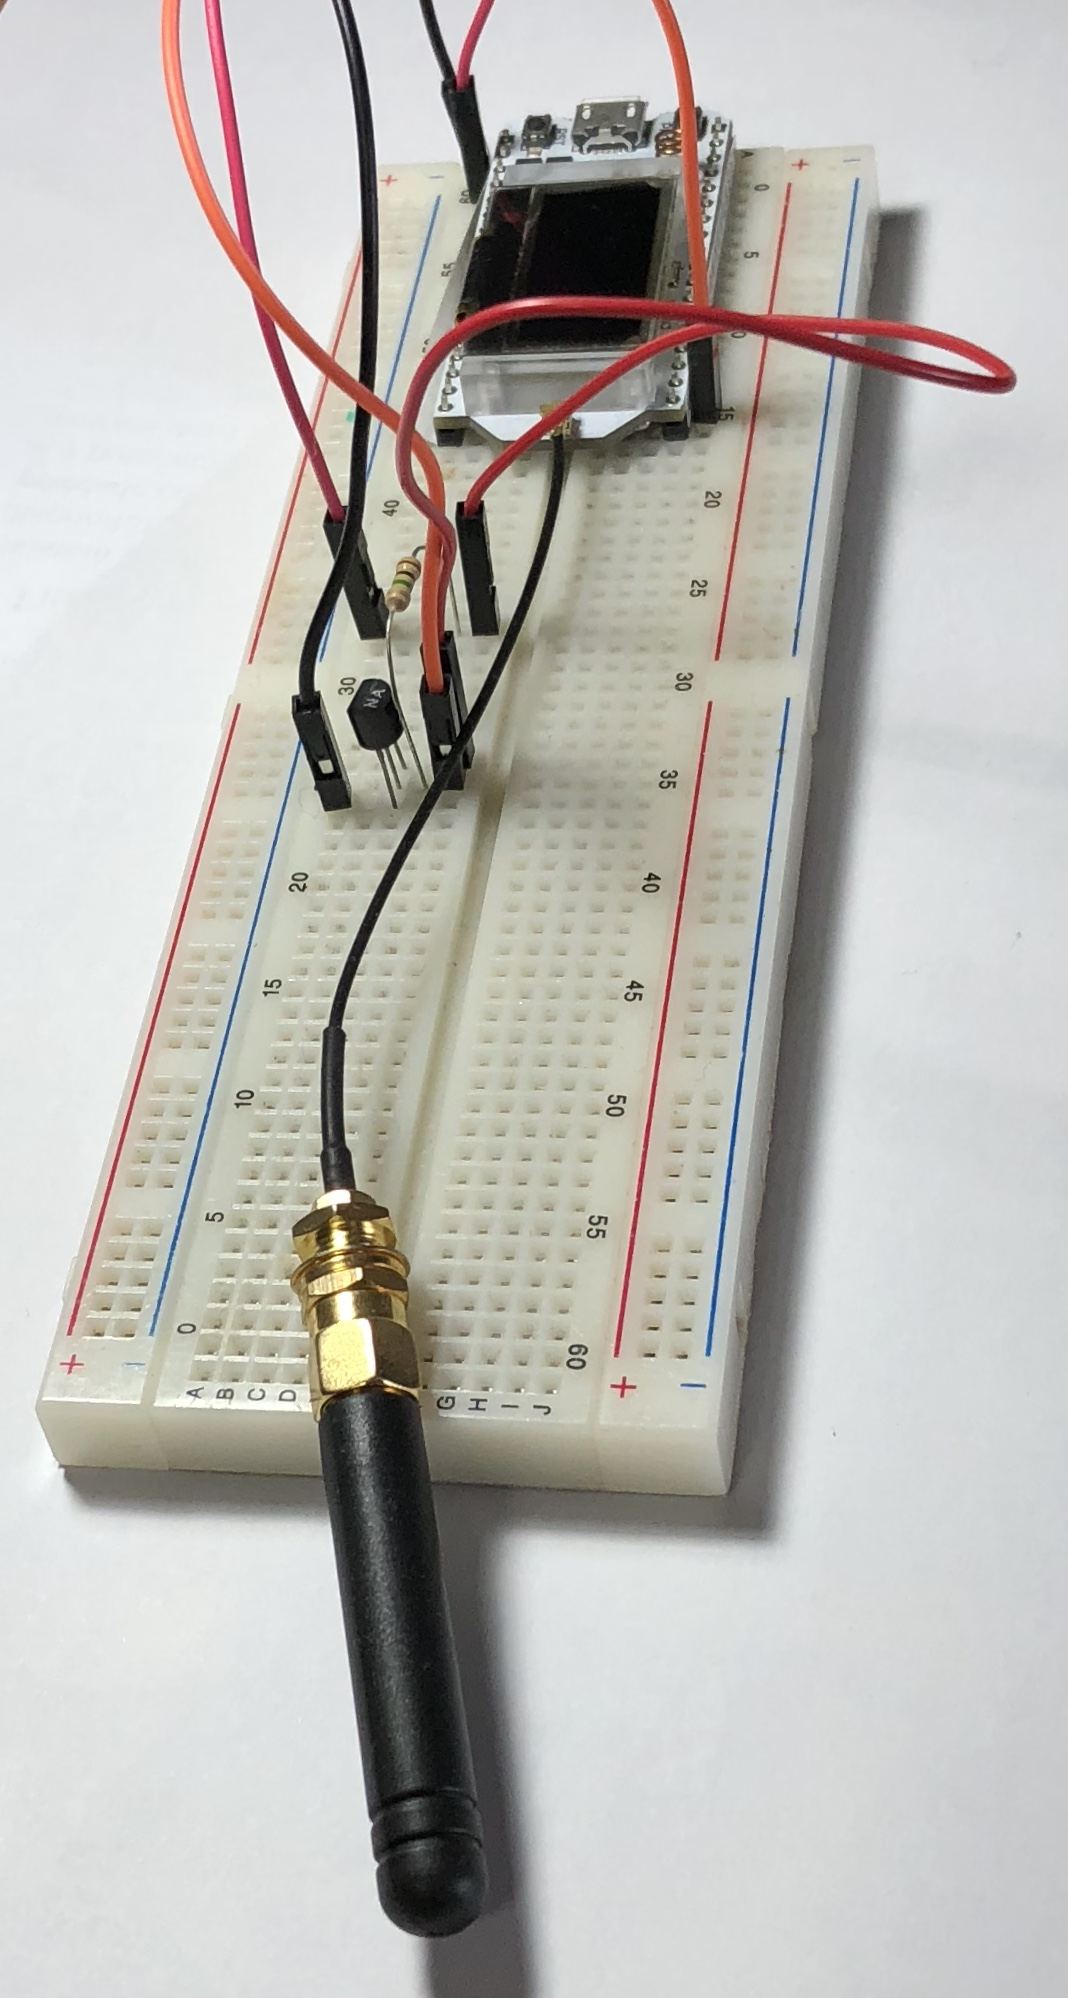
\includegraphics[width=0.5\textwidth]{temp1.jpg}
    \legend{Fonte: Autor}
    \label{fig:temp1}
\end{figure}

Montados os nós, foi então decidido a estrutura do código para rodar em cada um deles. Para o tratamento de troca de mensagens entre os dispositivos LoRa foi utilizada uma biblioteca chamada \textit{RadioHead}. Esta biblioteca é implementada em C++, e dá suporte tanto ao módulo RFM95W quando ao SX1278. A biblioteca é escolhida por ser implementada em C++, então os códigos podem rodar tanto no Arduino quanto no ESP32 que possui uma arquitetura semelhante ao Arduino Nano. A implementação dos códigos que rodam no nó de borda pode ser encontrada no repositório do \textit{GitHub} presente no anexo \ref{anexosoftware}, juntamente com o \textit{link} para a biblioteca \textit{RadioHead}.

\subsection{Protótipo do gateway}

O \textit{gateway} proposto utiliza o módulo da HopeRF RFM95W (ver seção 4.2) conectado aos pinos de propósito geral (GPIO) do \textit{Raspberry}. A ligação detalhada pode ser visualizada na imagem em anexo. O resultado dessa ligação é mostrado nas figuras \ref{fig:g1} e \ref{fig:g2}.

\begin{figure}[ht]
    \centering  
    \caption{Protótipo de \textit{gateway} para a aplicação utilizando \textit{Raspberry Pi}}
    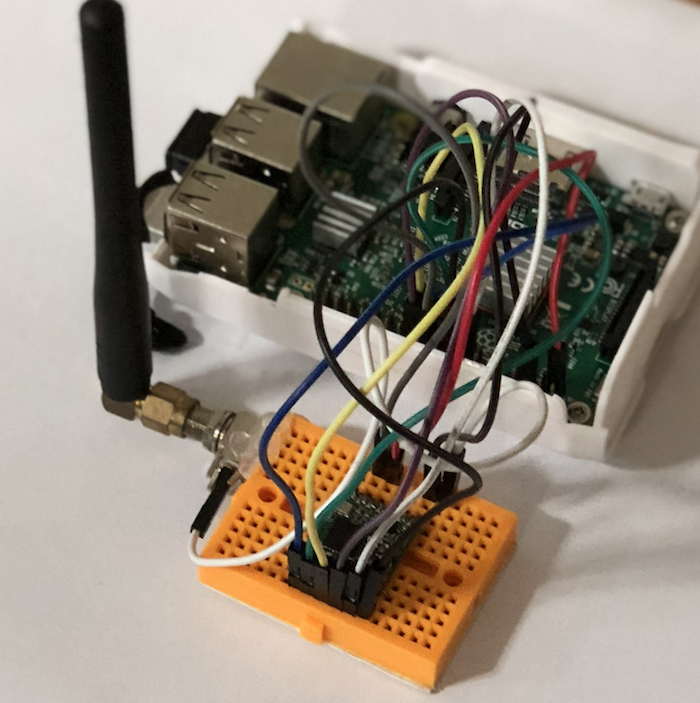
\includegraphics[width=0.5\textwidth]{g1.png}
    \legend{Fonte: Autor}
    \label{fig:g1}
\end{figure}
\begin{figure}[ht]
    \centering
    \caption{Protótipo de \textit{gateway} para a aplicação utilizando \textit{Raspberry Pi}}
    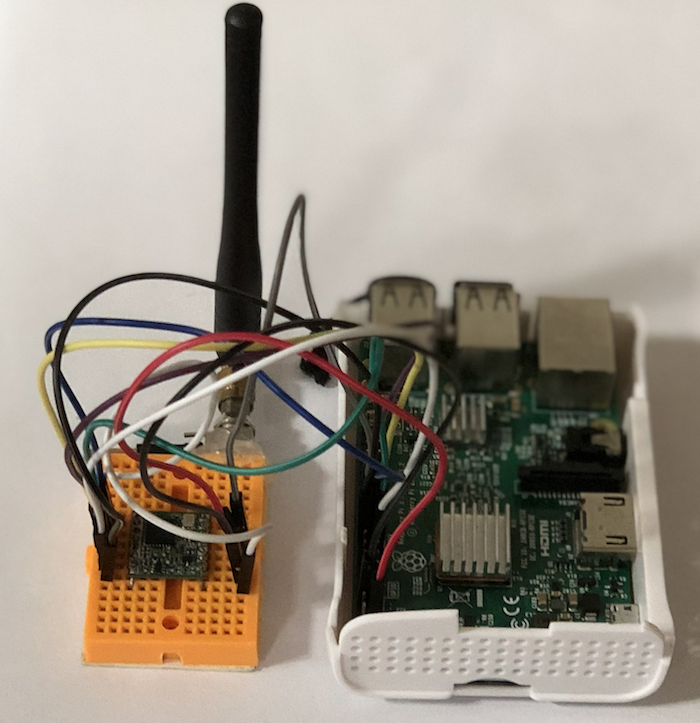
\includegraphics[width=0.5\textwidth]{g2.png}
    \legend{Fonte: Autor}
    \label{fig:g2}
\end{figure}
O código escrito para ser executado no gateway foi escrito em C++ utilizando também a biblioteca \textit{RadioHead} (ver seção 3.2) para o recebimento de pacotes LoRa. A plataforma de nuvem que recebe os dados do \textit{gateway} é a AWS IoT, descrita na próxima seção. Esta plataforma fornece um \textit{Software Development Kit} (SDK) escrito em C, sendo este o utilizado. O código executando no \textit{Rasberry} segue a seguinte estrutura:

\begin{algorithm}
\caption{Código do \textit{Gateway}}\label{gateway-code}
\begin{algorithmic}[1]
\Procedure{loop}{}
\State \textit{configure\_aws}()
\While {$\textit{exists connection with rf}$}
\If {$receive packet$}

\If {$packet is from Temperature Node$}
\State $temp \gets temp info from packet received$.
\State $p \gets \textit{makeJSON}(temp)$.
\State $\textit{persist\_in\_aws}(p)$.
\EndIf

\If {$packet is from GPS Node$}
\State $latitud \gets latitud info from packet received$.
\State $longitud \gets longitud info from packet received$.
\State $p \gets \textit{makeJSON}(latitud, longitud)$.
\State $\textit{persist\_in\_aws}(p)$.
\EndIf

\EndIf
\EndWhile
\EndProcedure

\Procedure{main}{}
\State \textit{configure\_rf}()
\State \textit{loop}()
\EndProcedure
\end{algorithmic}
\end{algorithm}

Na linha 15 do Algoritmo 1, o nó RFM95W é configurado utilizado as informações de frequência de operação, números de pinos em que as entradas estão conectadas e outras variáveis. É nessa parte que entra a biblioteca \textit{RadioHead}. Após feita a configuração e verificada a existência de um módulo lora ligado ao \textit{Raspberry}, também através das configurações realizadas pelo procedimento da linha 15, a linha 16 executará o \textit{loop} responsável por aguardar a chegada de pacotes. 

O procedimento invocado pela linha 16 do Algoritmo 1 primeiramente realizará a configuração da AWS IoT através do SDK fornecido pela Amazon. São fornecidos os certificados da conta criada na Amazon AWS IoT, também informando identificadores que representam o \textit{Raspberry Pi} na nuvem e outras configurações. Após isto, a linha 3 coloca o código em um laço de repetição até que não exista mais conexão com o módulo LoRa. Assim, quando um pacote é recebido, verificação feita na linha 4, é verificado se este pacote veio do nó de borda responsável pela localização ou se foi um pacote relacionado a temperatura. Esta verificação é feita, pois cada pacote deve ser configurado de maneira diferente para ser persistido na AWS. Caso seja um pacote de temperatura, é empacotada uma mensagem utilizando o formato JSON com o campo de temperatura, e persistido na AWS IoT, que pode ser verificado da linha 6 a 8. Caso seja um pacote com informações de coordenadas GPS, é empacotada uma mensagem no formato JSON contendo os campos de latitude e longitude, e também persistido na nuvem, podendo ser verificado da linha 10 a 13. 

A implementação em C++ do código do \textit{gateway} se encontra no repositório do \textit{GitHub} disponibilizado no anexo \ref{anexosoftware}, bem como um \textit{link} para o SDK escrito em C pela Amazon para a AWS IoT.

\subsection{Serviço de nuvem utilizado na aplicação}

O serviço de armazenamento em nuvem escolhido para compor a solução foi o AWS IoT. Nele é permitido que se crie uma "\textit{Thing}" (coisa) que está relacionada a sua rede \textit{Internet of Things}. No cenário dessa aplicação, a \textit{thing} será o \textit{gateway} construído com o \textit{Raspberry}, e que tem o nome na plataforma AWS IoT de RPi-Gateway. Após o registro desta "coisa", são gerados certificados que permitem o acesso dos SDKs fornecidos pela Amazon para publicar informações referentes a sua \textit{thing}. A figura \ref{fig:thing} mostra o \textit{Raspberry} com o módulo da HopeRF registrado como uma "coisa" na AWS.

A publicação de informação na plataforma é feita utilizando do protocolo MQTT (\textit{Message Queuing Telemetry Transport}), um protocolo considerado leve e utilizado em sensores e pequenos dispositivos. Esse protocolo é baseado no esquema de comunicação \textit{Publisher-Subscriber}. Também é possível utilizar uma interface de acesso REST para atualizar e recuperar as informações da nuvem através de métodos HTTP (GET, POST, UPDATE e outros). 

\begin{figure}[ht]
    \centering
    \caption{\textit{Thing} registrada na AWS IoT}
    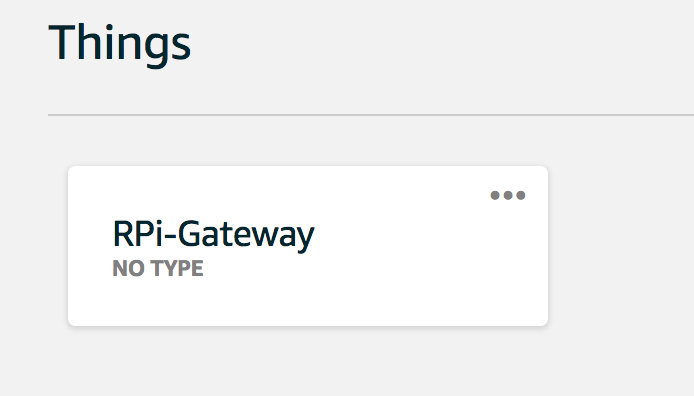
\includegraphics[width=0.5\textwidth]{thing.png}
    \legend{Fonte: Autor}
    \label{fig:thing}
\end{figure}

Os dados recebidos pela nuvem são encapsulados na forma de \textit{Shadow}, que utiliza da estrutura de objeto JSON (JavaScript Object Notation) para versionamento das informações. A figura \ref{fig:shadow} mostra as ultimas informações recebidas pelo \textit{gateway}.

\begin{figure}[ht]
    \centering    
    \caption{Informações recebidas pelos nós e armazenados na \textit{Shadow}}
    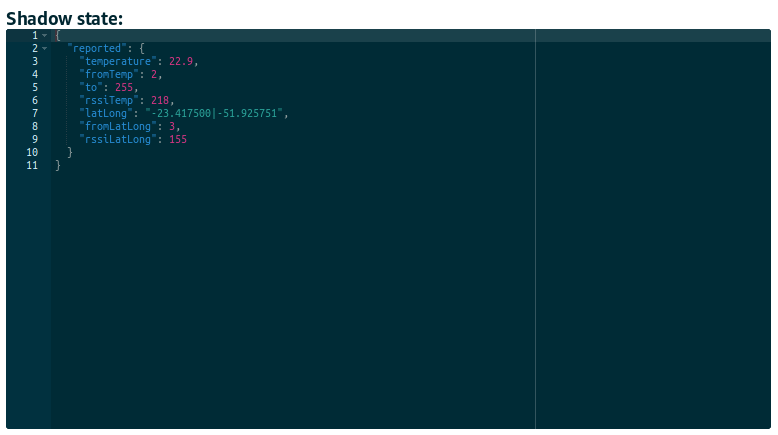
\includegraphics[width=0.5\textwidth]{shadow.png}
    \legend{Fonte: Autor}
    \label{fig:shadow}
\end{figure}

\subsection{Aplicativo MannaWare}

Com os dados publicados no serviço de nuvem da Amazon, foi desenvolvido então um protótipo de aplicativo web para fornecer essas informações para um usuário final da solução. Pode-se pensar, no cenário desse trabalho, que um possível usuário final é o fazendeiro que possui a aplicação para monitoramento de sua fazenda.

Como são dois dispositivos de borda coletando informações de temperatura e de localização, e um \textit{gateway} para receber os dados desses dispositivos, foi desenvolvido um aplicativo em que no menu lateral tem a opção de selecionar o \textit{gateway} que se deseja consultar, e quando aberta esta página são mostrados \textit{cards} contendo as informações de cada dispositivo de borda que se comunica a este \textit{gateway}.A imagem \ref{fig:screenshotmannaware} representa esta página.

\begin{figure}[ht]
    \centering
    \caption{Página com as informações dos dispositivos de borda no aplicativo MannaWare}
    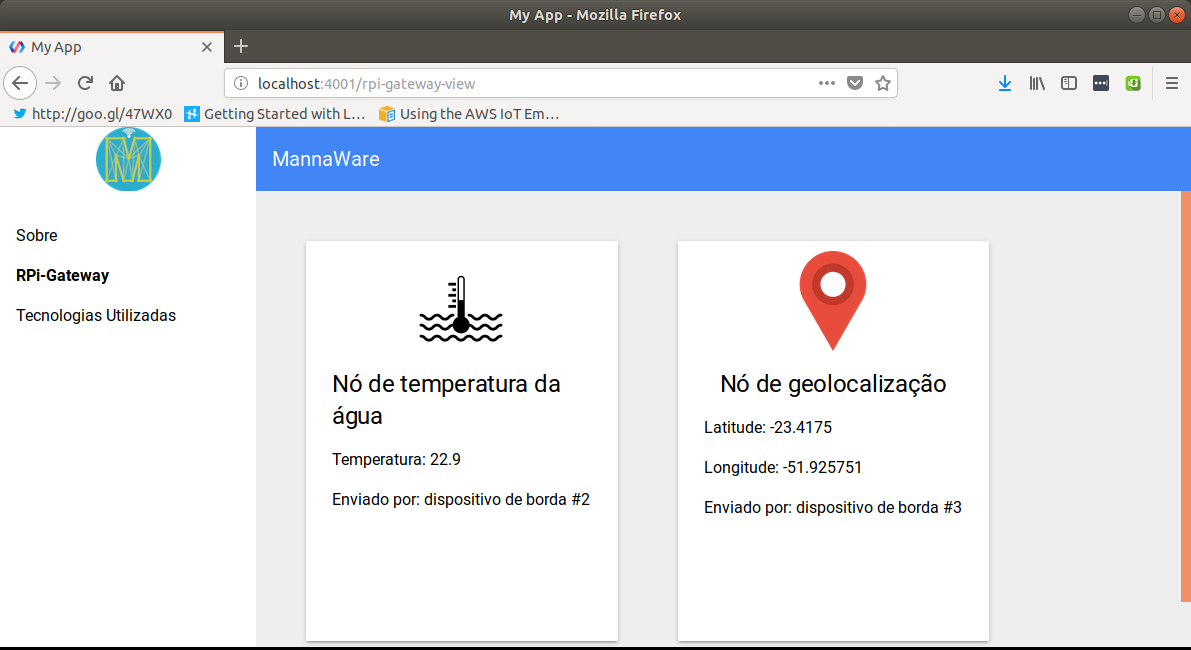
\includegraphics[width=1\textwidth]{screenshot-mannaware.png}
    \legend{Fonte: Autor}
    \label{fig:screenshotmannaware}
\end{figure}

Esta aplicação foi desenvolvida utilizando-se a biblioteca Polymer, que é uma biblioteca desenvolvida para a criação de \textit{front-ends} web utilizando o conceito \textit{WebComponentes} de encapsulamento de componentes web. Também foi utilizado o SDK \textit{Python} da AWS IoT fornecido pela própria Amazon, para recuperar os dados armazenados na nuvem. O código do aplicativo pode ser encontrado no repositório presente no anexo \ref{anexosoftware}.

\section{Desafios de desenvolvimento}

Ao longo da montagem de cada elemento da rede foram levantados alguns desafios. Prototipar uma aplicação no cenário da internet das coisas abordando todas etapas da infraestrutura IoT não é trivial, e nem sempre vem com uma solução \textit{plug and play}. A seguir serão descritos os desafios enfrentados para a construção da solução de monitoramento.

\subsection{Desafios de hardware}

O módulo de rádio RFM95W adquirido para o desenvolvimento deste projeto não é um módulo encapsulado a um microcontrolador, não vem com pinos de encaixe em \textit{protoboard} embutidos e nem com uma antena já instalada no circuito. Dessa forma, para utilizá-lo teve que se soldar pinos de cobre em suas entradas, para assim poder conectar \textit{jumpers} a ele com o intuíto de realizar a comunicação com o Arduino e o Raspberry. 

Soldar pinos de entrada para serem conectados a \textit{jumpers} não é a solução mais aconselhada para esse tipo de módulo de rádio, pois pode diminuir drasticamente seu desempenho de comunicação. Uma abordagem melhor é utilizar algum \textit{software} para desenhar um circuito customizado de acordo com suas necessidades e levar até uma casa especializada em impressão de circuitos e então confeccionar uma placa em que o módulo de rádio será embutido. Por falta de mão de obra especializada na região, não foi adotada essa estratégia.

O \textit{shield} GPS disponível para a fabricação de um dos dispositivos de borda não possui uma boa recepção de sinal, o que gerou dificuldade em realizar testes com a solução de monitoramento desenvolvida.

\subsection{Desafios de software}

O principal desafio relacionado a \textit{software} encontrado no desenvolvimento foi o SDK \textit{JavaScript} fornecido pela Amazon para a recuperação das informações de sua plataforma de nuvem. Foi realizada uma tentativa de uso do SDK escrito em \textit{JavaScript}, pois o Polymer é integrado a esta linguage.O SDK possui limitações e não funciona de forma correta em aplicações que rodam em \textit{browser}. Assim, não foi possível fazer a recuperação dos dados presentes na nuvem direto pela aplicação MannaWare. Para contornar esse problema, utilizando o SDK \textit{Python} AWS foi escrito um \textit{script} que se comporta como um servidor local e se comunica através de \textit{Socket} com o apicativo MannaWare. Este \textit{script} ao receber um novo estado do \textit{shadow} do \textit{gateway}, comunica a mensagem ao MannaWare.

Outro desafio relacionado a software é a escassa disponibilidade de bibliotecas que tratam a ligação de módulos de rádio como o RFM95W e o \textit{Raspberry Pi}. Escrever um código para essa comunicação não é trivial, e sua implementação tomaria todo o tempo disponível para o desenvolvimento da aplicação como um todo, distorcendo o objetivo a ser alcançado com esse trabalho.


\setcounter{section}{0}
\chapter*[Capítulo 5]{Capítulo 5} \label{capitulo5}
\addcontentsline{toc}{chapter}{Capítulo 5}
\section{Conclusão}

A aplicação proposta para estudo de caso desse trabalho tem como objetivo monitorar parâmetros em ambientes rurais, porém a aplicação pode ser testada para monitorar outro tipo de ambiente que não o rural. Ao mudar o cenário da aplicação, haverá mudanças nas variáveis e objetos a serem monitorados, porém o cerne da infraestrutura permanece imutável, ou seja, a comunicação entre os nós de borda e o \textit{gateway} permanece a mesma, e a estratégia de persistência de dados na plataforma em nuvem e sua recuperação pelo aplicativo para o usuário final permanecem também da mesma forma. 

Caso o ambiente exija uma rede com comunicação heterogênea, então haverá a necessidade de se ligar um módulo de radio receptor a mais no \textit{Raspberry Pi} e reformular o código que roda nele para aceitar pacotes advindos de outras tecnologias de comunicação que não são LoRa. Uma outra estratégia para esse caso é ter um \textit{gateway} diferente que tenha a conexão com os nós que conversam outros protocolos. Como um exemplo, caso o cenário exija um nó de borda que transmita informações utilizando o protocolo \textit{ZigBee} então será utilizado um outro \textit{gateway} que possua recepção para \textit{ZigBee}. 

Espera-se que utilizando a mesma tecnologia de comunicação, a aplicação de monitoramento aceite a inserção de novos nós de borda coletando informações de novos parâmetros inseridos no contexto da aplicação.

O protótipo desenvolvido para este trabalho cobriu todas as partes da infraestrutura definida para a Internet das coisas, uma vez que forneceu a implementação de nós de borda, de um \textit{gateway} e sua comunicação com uma plataforma em nuvem, e além disso um aplicativo chamado MannaWare que tem o objetivo de apresentar as informações coletadas pela rede para o usuário final. Assim conclui-se que a solução se encaixa na organização da infraestrutura IoT.

O protótipo tem um caráter científico de descoberta e exploração. Assim, seu desenvolvimento foi composto de soluções prontas no mercado. Isto é, para a confecção dos nós de borda foram utilizados microcontroladores genéricos como o ESP32 e o Arduino Uno, o \textit{gateway} foi implementado utilizando um \textit{Raspberry Pi 3}, os módulos de rádio LoRa foram soldados manualmente. O armazenamento das informações em nuvem foi feito através da Amazon. Essa composição de produtos prontos no mercado são excelentes para o estudo e desenvolvimento de protótipos, porém não é o ideal para o desenvolvimento de um produto final, uma vez que esses produtos prontos moldam a sua aplicação a se tornar genérica. Assim, conclui-se que para gerar um produto a ser comercializado a melhor estratégia é a fabricação de todos os componentes que estarão disponíveis na rede IoT, desde o nó de borda até o armazenamento em nuvem.

\section{Trabalhos futuros}

Construído um prototipo que abrange todas as partes presentes na infraestrutura da Internet das Coisas, um leque de trabalhos futuros se abre. Serão listadas algumas tarefas a se desenvolver futuramente com objetivo de melhorar este trabalho:
\begin{itemize}
\item Aplicação da solução em um cenário real de ambiente rural;
\item Produção de circuitos impressos para o encapsulamento do rádio LoRa RFM95W;
\item Produção de dispositivos de borda próprios encapsulado com sensores previamente escolhidos;
\item Estudo relacionado a antenas e sua influência na distância de comunicação entre dispositivos que utilizam LoRa;
\item Analise de consumo de energia dos dispositivos desenvolvidos;
\item Desenvolvimento de uma biblioteca própria de comunicação entre módulos lora e hardwares como microcontroladores e microcomputadores;
\item Desenvolvimento de um \textit{gateway} que seja capaz de aceitar uma rede heterogênea, como é um dos propósitos de uma rede IoT. Sendo assim, o desenvolvimento leva em conta a inserção de mais módulos de recepção compatíveis com outros protocolos;
\item Criação de uma solução própria de armazenamento em nuvem, desvinculando a aplicação de soluções prontas fornecidas no mercado;
\item Desenvolvimento de um aplicativo mais completo que forneça as informações necessárias ao usuário, bem como a inclusão de ferramentas de análise estatística como a média dos dados armazenados na nuvem. Possibilitar o usuário a atuar através da rede IoT, permitindo o disparo de ações mediante as informações fornecidas a ele. 
\end{itemize}

% \section{Resumo}
% Este capítulo apresenta o fechamento de todo o estudo de caso realizado. Nele são escolhidas duas variáveis a serem analisadas no ambiente rural e é mostrado o processo de criação da rede IoT para o monitoramento destas variáveis. São justificadas as escolhas de hardware e apresentados os resultados da criação da aplicação. Aponta-se os desafios enfrentados no desenvolvimento, é feita uma conclusão a partir dos resultados obtidos e são levantados possíveis trabalhos futuros para o melhoramento da aplicação.
%Este documento e seu código-fonte são exemplos de referência de uso da classe
%\textsf{abntex2} e do pacote \textsf{abntex2cite}. O documento 
%exemplifica a elaboração de trabalho acadêmico (tese, dissertação e outros do
%gênero) produzido conforme a ABNT NBR 14724:2011 \emph{Informação e documentação
%- Trabalhos acadêmicos - Apresentação}.
%
%A expressão ``Modelo Canônico'' é utilizada para indicar que \abnTeX\ não é
%modelo específico de nenhuma universidade ou instituição, mas que implementa tão
%somente os requisitos das normas da ABNT. Uma lista completa das normas
%observadas pelo \abnTeX\ é apresentada em \citeonline{abntex2classe}.
%
%Sinta-se convidado a participar do projeto \abnTeX! Acesse o site do projeto em
%\url{http://www.abntex.net.br/}. Também fique livre para conhecer,
%estudar, alterar e redistribuir o trabalho do \abnTeX, desde que os arquivos
%modificados tenham seus nomes alterados e que os créditos sejam dados aos
%autores originais, nos termos da ``The \LaTeX\ Project Public
%License''\footnote{\url{http://www.latex-project.org/lppl.txt}}.
%
%Encorajamos que sejam realizadas customizações específicas deste exemplo para
%universidades e outras instituições --- como capas, folha de aprovação, etc.
%Porém, recomendamos que ao invés de se alterar diretamente os arquivos do
%\abnTeX, distribua-se arquivos com as respectivas customizações.
%Isso permite que futuras versões do \abnTeX~não se tornem automaticamente
%incompatíveis com as customizações promovidas. Consulte
%\citeonline{abntex2-wiki-como-customizar} par mais informações.
%
%Este documento deve ser utilizado como complemento dos manuais do \abnTeX\ 
%\cite{abntex2classe,abntex2cite,abntex2cite-alf} e da classe \textsf{memoir}
%\cite{memoir}. 
%
%Esperamos, sinceramente, que o \abnTeX\ aprimore a qualidade do trabalho que
%você produzirá, de modo que o principal esforço seja concentrado no principal:
%na contribuição científica.
%
%Equipe \abnTeX 
%
%Lauro César Araujo
%
%% ----------------------------------------------------------
%% PARTE
%% ----------------------------------------------------------
%\part{Preparação da pesquisa}
%% ----------------------------------------------------------
%
%% ---
%% Capitulo com exemplos de comandos inseridos de arquivo externo 
%% ---
%%% abtex2-modelo-include-comandos.tex, v-1.9.6 laurocesar
%% Copyright 2012-2016 by abnTeX2 group at http://www.abntex.net.br/ 
%%
%% This work may be distributed and/or modified under the
%% conditions of the LaTeX Project Public License, either version 1.3
%% of this license or (at your option) any later version.
%% The latest version of this license is in
%%   http://www.latex-project.org/lppl.txt
%% and version 1.3 or later is part of all distributions of LaTeX
%% version 2005/12/01 or later.
%%
%% This work has the LPPL maintenance status `maintained'.
%% 
%% The Current Maintainer of this work is the abnTeX2 team, led
%% by Lauro César Araujo. Further information are available on 
%% http://www.abntex.net.br/
%%
%% This work consists of the files abntex2-modelo-include-comandos.tex
%% and abntex2-modelo-img-marca.pdf
%%

% ---
% Este capítulo, utilizado por diferentes exemplos do abnTeX2, ilustra o uso de
% comandos do abnTeX2 e de LaTeX.
% ---
 
\chapter{Resultados de comandos}\label{cap_exemplos}

\chapterprecis{Isto é uma sinopse de capítulo. A ABNT não traz nenhuma
normatização a respeito desse tipo de resumo, que é mais comum em romances 
e livros técnicos.}\index{sinopse de capítulo}

% ---
\section{Codificação dos arquivos: UTF8}
% ---

A codificação de todos os arquivos do \abnTeX\ é \texttt{UTF8}. É necessário que
você utilize a mesma codificação nos documentos que escrever, inclusive nos
arquivos de base bibliográficas |.bib|.

% ---
\section{Citações diretas}
\label{sec-citacao}
% ---

\index{citações!diretas}Utilize o ambiente \texttt{citacao} para incluir
citações diretas com mais de três linhas:

\begin{citacao}
As citações diretas, no texto, com mais de três linhas, devem ser
destacadas com recuo de 4 cm da margem esquerda, com letra menor que a do texto
utilizado e sem as aspas. No caso de documentos datilografados, deve-se
observar apenas o recuo \cite[5.3]{NBR10520:2002}.
\end{citacao}

Use o ambiente assim:

\begin{verbatim}
\begin{citacao}
As citações diretas, no texto, com mais de três linhas [...] deve-se observar
apenas o recuo \cite[5.3]{NBR10520:2002}.
\end{citacao}
\end{verbatim}

O ambiente \texttt{citacao} pode receber como parâmetro opcional um nome de
idioma previamente carregado nas opções da classe (\autoref{sec-hifenizacao}). Nesse
caso, o texto da citação é automaticamente escrito em itálico e a hifenização é
ajustada para o idioma selecionado na opção do ambiente. Por exemplo:

\begin{verbatim}
\begin{citacao}[english]
Text in English language in italic with correct hyphenation.
\end{citacao}
\end{verbatim}

Tem como resultado:

\begin{citacao}[english]
Text in English language in italic with correct hyphenation.
\end{citacao}

\index{citações!simples}Citações simples, com até três linhas, devem ser
incluídas com aspas. Observe que em \LaTeX as aspas iniciais são diferentes das
finais: ``Amor é fogo que arde sem se ver''.

% ---
\section{Notas de rodapé}
% ---

As notas de rodapé são detalhadas pela NBR 14724:2011 na seção 5.2.1\footnote{As
notas devem ser digitadas ou datilografadas dentro das margens, ficando
separadas do texto por um espaço simples de entre as linhas e por filete de 5
cm, a partir da margem esquerda. Devem ser alinhadas, a partir da segunda linha
da mesma nota, abaixo da primeira letra da primeira palavra, de forma a destacar
o expoente, sem espaço entre elas e com fonte menor
\citeonline[5.2.1]{NBR14724:2011}.}\footnote{Caso uma série de notas sejam
criadas sequencialmente, o \abnTeX\ instrui o \LaTeX\ para que uma vírgula seja
colocada após cada número do expoente que indica a nota de rodapé no corpo do
texto.}\footnote{Verifique se os números do expoente possuem uma vírgula para
dividi-los no corpo do texto.}. 


% ---
\section{Tabelas}
% ---

\index{tabelas}A \autoref{tab-nivinv} é um exemplo de tabela construída em
\LaTeX.

\begin{table}[htb]
\ABNTEXfontereduzida
\caption[Níveis de investigação]{Níveis de investigação.}
\label{tab-nivinv}
\begin{tabular}{p{2.6cm}|p{6.0cm}|p{2.25cm}|p{3.40cm}}
  %\hline
   \textbf{Nível de Investigação} & \textbf{Insumos}  & \textbf{Sistemas de Investigação}  & \textbf{Produtos}  \\
    \hline
    Meta-nível & Filosofia\index{filosofia} da Ciência  & Epistemologia &
    Paradigma  \\
    \hline
    Nível do objeto & Paradigmas do metanível e evidências do nível inferior &
    Ciência  & Teorias e modelos \\
    \hline
    Nível inferior & Modelos e métodos do nível do objeto e problemas do nível inferior & Prática & Solução de problemas  \\
   % \hline
\end{tabular}
\legend{Fonte: \citeonline{van86}}
\end{table}

Já a \autoref{tabela-ibge} apresenta uma tabela criada conforme o padrão do
\citeonline{ibge1993} requerido pelas normas da ABNT para documentos técnicos e
acadêmicos.

\begin{table}[htb]
\IBGEtab{%
  \caption{Um Exemplo de tabela alinhada que pode ser longa
  ou curta, conforme padrão IBGE.}%
  \label{tabela-ibge}
}{%
  \begin{tabular}{ccc}
  \toprule
   Nome & Nascimento & Documento \\
  \midrule \midrule
   Maria da Silva & 11/11/1111 & 111.111.111-11 \\
  \midrule 
   João Souza & 11/11/2111 & 211.111.111-11 \\
  \midrule 
   Laura Vicuña & 05/04/1891 & 3111.111.111-11 \\
  \bottomrule
\end{tabular}%
}{%
  \fonte{Produzido pelos autores.}%
  \nota{Esta é uma nota, que diz que os dados são baseados na
  regressão linear.}%
  \nota[Anotações]{Uma anotação adicional, que pode ser seguida de várias
  outras.}%
  }
\end{table}


% ---
\section{Figuras}
% ---

\index{figuras}Figuras podem ser criadas diretamente em \LaTeX,
como o exemplo da \autoref{fig_circulo}.

\begin{figure}[htb]
	\caption{\label{fig_circulo}A delimitação do espaço}
	\begin{center}
	    \setlength{\unitlength}{5cm}
		\begin{picture}(1,1)
		\put(0,0){\line(0,1){1}}
		\put(0,0){\line(1,0){1}}
		\put(0,0){\line(1,1){1}}
		\put(0,0){\line(1,2){.5}}
		\put(0,0){\line(1,3){.3333}}
		\put(0,0){\line(1,4){.25}}
		\put(0,0){\line(1,5){.2}}
		\put(0,0){\line(1,6){.1667}}
		\put(0,0){\line(2,1){1}}
		\put(0,0){\line(2,3){.6667}}
		\put(0,0){\line(2,5){.4}}
		\put(0,0){\line(3,1){1}}
		\put(0,0){\line(3,2){1}}
		\put(0,0){\line(3,4){.75}}
		\put(0,0){\line(3,5){.6}}
		\put(0,0){\line(4,1){1}}
		\put(0,0){\line(4,3){1}}
		\put(0,0){\line(4,5){.8}}
		\put(0,0){\line(5,1){1}}
		\put(0,0){\line(5,2){1}}
		\put(0,0){\line(5,3){1}}
		\put(0,0){\line(5,4){1}}
		\put(0,0){\line(5,6){.8333}}
		\put(0,0){\line(6,1){1}}
		\put(0,0){\line(6,5){1}}
		\end{picture}
	\end{center}
	\legend{Fonte: os autores}
\end{figure}

Ou então figuras podem ser incorporadas de arquivos externos, como é o caso da
\autoref{fig_grafico}. Se a figura que ser incluída se tratar de um diagrama, um
gráfico ou uma ilustração que você mesmo produza, priorize o uso de imagens
vetoriais no formato PDF. Com isso, o tamanho do arquivo final do trabalho será
menor, e as imagens terão uma apresentação melhor, principalmente quando
impressas, uma vez que imagens vetorias são perfeitamente escaláveis para
qualquer dimensão. Nesse caso, se for utilizar o Microsoft Excel para produzir
gráficos, ou o Microsoft Word para produzir ilustrações, exporte-os como PDF e
os incorpore ao documento conforme o exemplo abaixo. No entanto, para manter a
coerência no uso de software livre (já que você está usando \LaTeX e \abnTeX),
teste a ferramenta \textsf{InkScape}\index{InkScape}
(\url{http://inkscape.org/}). Ela é uma excelente opção de código-livre para
produzir ilustrações vetoriais, similar ao CorelDraw\index{CorelDraw} ou ao Adobe
Illustrator\index{Adobe Illustrator}. De todo modo, caso não seja possível
utilizar arquivos de imagens como PDF, utilize qualquer outro formato, como
JPEG, GIF, BMP, etc. Nesse caso, você pode tentar aprimorar as imagens
incorporadas com o software livre \textsf{Gimp}\index{Gimp}
(\url{http://www.gimp.org/}). Ele é uma alternativa livre ao Adobe
Photoshop\index{Adobe Photoshop}.

\begin{figure}[htb]
	\caption{\label{fig_grafico}Gráfico produzido em Excel e salvo como PDF}
	\begin{center}
	    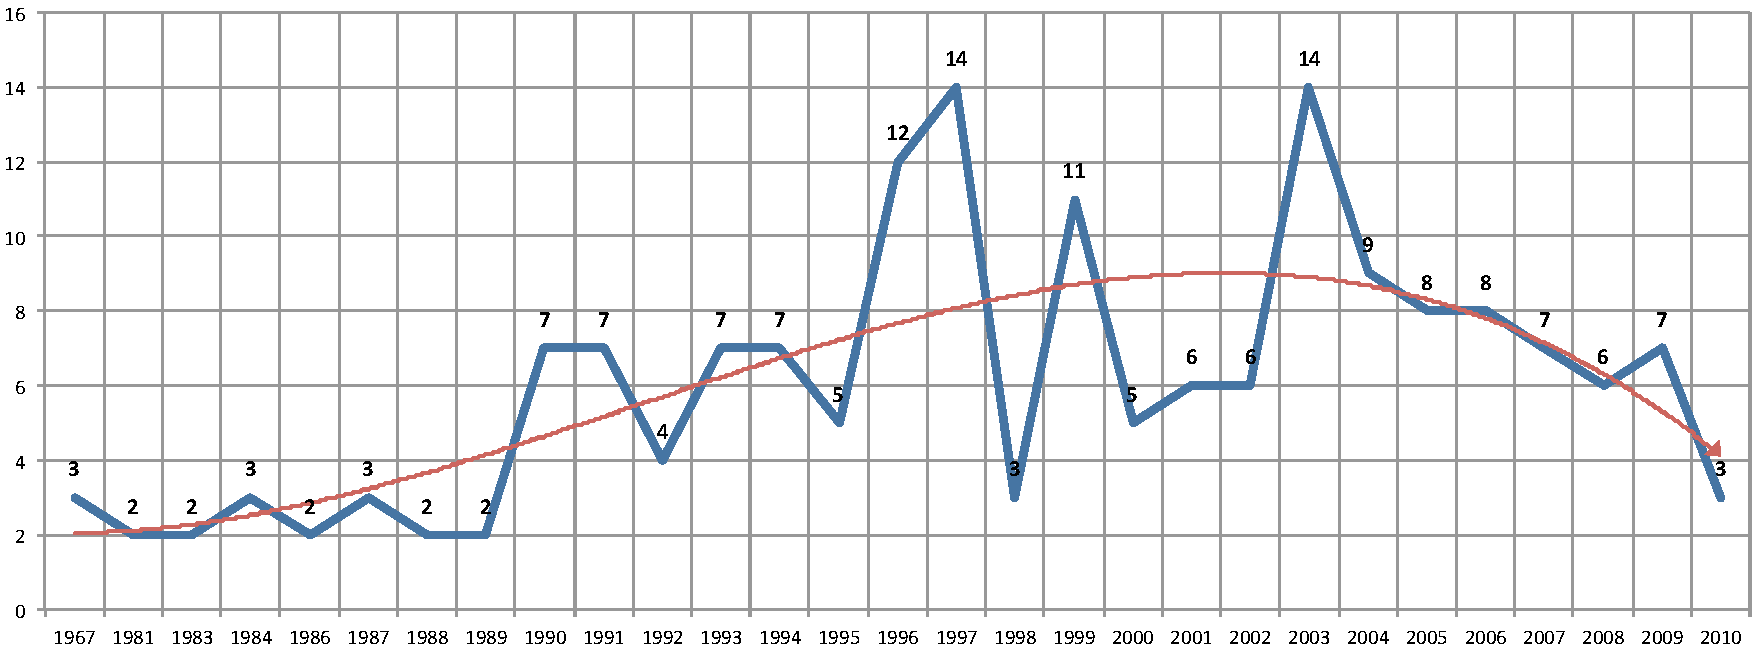
\includegraphics[scale=0.5]{abntex2-modelo-img-grafico.pdf}
	\end{center}
	\legend{Fonte: \citeonline[p. 24]{araujo2012}}
\end{figure}

% ---
\subsection{Figuras em \emph{minipages}}
% ---

\emph{Minipages} são usadas para inserir textos ou outros elementos em quadros
com tamanhos e posições controladas. Veja o exemplo da
\autoref{fig_minipage_imagem1} e da \autoref{fig_minipage_grafico2}.

\begin{figure}[htb]
 \label{teste}
 \centering
  \begin{minipage}{0.4\textwidth}
    \centering
    \caption{Imagem 1 da minipage} \label{fig_minipage_imagem1}
    
\includegraphics[scale=0.9]{abntex2-modelo-img-marca.pdf}
    \legend{Fonte: Produzido pelos autores}
  \end{minipage}
  \hfill
  \begin{minipage}{0.4\textwidth}
    \centering
    \caption{Grafico 2 da minipage} \label{fig_minipage_grafico2}
    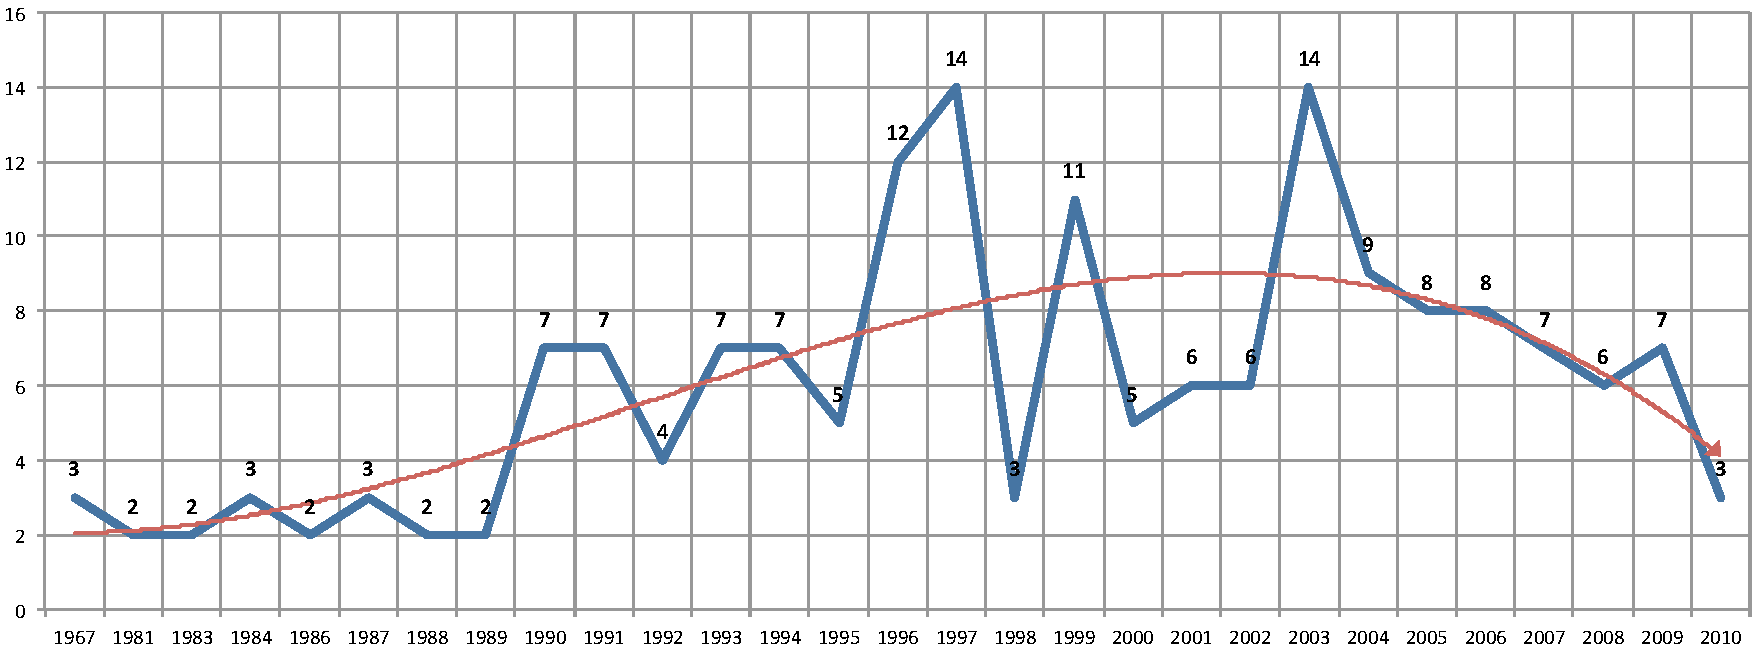
\includegraphics[scale=0.2]{abntex2-modelo-img-grafico.pdf}
    \legend{Fonte: \citeonline[p. 24]{araujo2012}}
  \end{minipage}
\end{figure}

Observe que, segundo a \citeonline[seções 4.2.1.10 e 5.8]{NBR14724:2011}, as
ilustrações devem sempre ter numeração contínua e única em todo o documento:

\begin{citacao}
Qualquer que seja o tipo de ilustração, sua identificação aparece na parte
superior, precedida da palavra designativa (desenho, esquema, fluxograma,
fotografia, gráfico, mapa, organograma, planta, quadro, retrato, figura,
imagem, entre outros), seguida de seu número de ordem de ocorrência no texto,
em algarismos arábicos, travessão e do respectivo título. Após a ilustração, na
parte inferior, indicar a fonte consultada (elemento obrigatório, mesmo que
seja produção do próprio autor), legenda, notas e outras informações
necessárias à sua compreensão (se houver). A ilustração deve ser citada no
texto e inserida o mais próximo possível do trecho a que se
refere. \cite[seções 5.8]{NBR14724:2011}
\end{citacao}

% ---
\section{Expressões matemáticas}
% ---

\index{expressões matemáticas}Use o ambiente \texttt{equation} para escrever
expressões matemáticas numeradas:

\begin{equation}
  \forall x \in X, \quad \exists \: y \leq \epsilon
\end{equation}

Escreva expressões matemáticas entre \$ e \$, como em $ \lim_{x \to \infty}
\exp(-x) = 0 $, para que fiquem na mesma linha.

Também é possível usar colchetes para indicar o início de uma expressão
matemática que não é numerada.

\[
\left|\sum_{i=1}^n a_ib_i\right|
\le
\left(\sum_{i=1}^n a_i^2\right)^{1/2}
\left(\sum_{i=1}^n b_i^2\right)^{1/2}
\]

Consulte mais informações sobre expressões matemáticas em
\url{https://github.com/abntex/abntex2/wiki/Referencias}.

% ---
\section{Enumerações: alíneas e subalíneas}
% ---

\index{alíneas}\index{subalíneas}\index{incisos}Quando for necessário enumerar
os diversos assuntos de uma seção que não possua título, esta deve ser
subdividida em alíneas \cite[4.2]{NBR6024:2012}:

\begin{alineas}

  \item os diversos assuntos que não possuam título próprio, dentro de uma mesma
  seção, devem ser subdivididos em alíneas; 
  
  \item o texto que antecede as alíneas termina em dois pontos;
  \item as alíneas devem ser indicadas alfabeticamente, em letra minúscula,
  seguida de parêntese. Utilizam-se letras dobradas, quando esgotadas as
  letras do alfabeto;

  \item as letras indicativas das alíneas devem apresentar recuo em relação à
  margem esquerda;

  \item o texto da alínea deve começar por letra minúscula e terminar em
  ponto-e-vírgula, exceto a última alínea que termina em ponto final;

  \item o texto da alínea deve terminar em dois pontos, se houver subalínea;

  \item a segunda e as seguintes linhas do texto da alínea começa sob a
  primeira letra do texto da própria alínea;
  
  \item subalíneas \cite[4.3]{NBR6024:2012} devem ser conforme as alíneas a
  seguir:

  \begin{alineas}
     \item as subalíneas devem começar por travessão seguido de espaço;

     \item as subalíneas devem apresentar recuo em relação à alínea;

     \item o texto da subalínea deve começar por letra minúscula e terminar em
     ponto-e-vírgula. A última subalínea deve terminar em ponto final, se não
     houver alínea subsequente;

     \item a segunda e as seguintes linhas do texto da subalínea começam sob a
     primeira letra do texto da própria subalínea.
  \end{alineas}
  
  \item no \abnTeX\ estão disponíveis os ambientes \texttt{incisos} e
  \texttt{subalineas}, que em suma são o mesmo que se criar outro nível de
  \texttt{alineas}, como nos exemplos à seguir:
  
  \begin{incisos}
    \item \textit{Um novo inciso em itálico};
  \end{incisos}
  
  \item Alínea em \textbf{negrito}:
  
  \begin{subalineas}
    \item \textit{Uma subalínea em itálico};
    \item \underline{\textit{Uma subalínea em itálico e sublinhado}}; 
  \end{subalineas}
  
  \item Última alínea com \emph{ênfase}.
  
\end{alineas}

% ---
\section{Espaçamento entre parágrafos e linhas}
% ---

\index{espaçamento!dos parágrafos}O tamanho do parágrafo, espaço entre a margem
e o início da frase do parágrafo, é definido por:

\begin{verbatim}
   \setlength{\parindent}{1.3cm}
\end{verbatim}

\index{espaçamento!do primeiro parágrafo}Por padrão, não há espaçamento no
primeiro parágrafo de cada início de divisão do documento
(\autoref{sec-divisoes}). Porém, você pode definir que o primeiro parágrafo
também seja indentado, como é o caso deste documento. Para isso, apenas inclua o
pacote \textsf{indentfirst} no preâmbulo do documento:

\begin{verbatim}
   \usepackage{indentfirst}      % Indenta o primeiro parágrafo de cada seção.
\end{verbatim}

\index{espaçamento!entre os parágrafos}O espaçamento entre um parágrafo e outro
pode ser controlado por meio do comando:

\begin{verbatim}
  \setlength{\parskip}{0.2cm}  % tente também \onelineskip
\end{verbatim}

\index{espaçamento!entre as linhas}O controle do espaçamento entre linhas é
definido por:

\begin{verbatim}
  \OnehalfSpacing       % espaçamento um e meio (padrão); 
  \DoubleSpacing        % espaçamento duplo
  \SingleSpacing        % espaçamento simples	
\end{verbatim}

Para isso, também estão disponíveis os ambientes:

\begin{verbatim}
  \begin{SingleSpace} ...\end{SingleSpace}
  \begin{Spacing}{hfactori} ... \end{Spacing}
  \begin{OnehalfSpace} ... \end{OnehalfSpace}
  \begin{OnehalfSpace*} ... \end{OnehalfSpace*}
  \begin{DoubleSpace} ... \end{DoubleSpace}
  \begin{DoubleSpace*} ... \end{DoubleSpace*} 
\end{verbatim}

Para mais informações, consulte \citeonline[p. 47-52 e 135]{memoir}.

% ---
\section{Inclusão de outros arquivos}\label{sec-include}
% ---

É uma boa prática dividir o seu documento em diversos arquivos, e não
apenas escrever tudo em um único. Esse recurso foi utilizado neste
documento. Para incluir diferentes arquivos em um arquivo principal,
de modo que cada arquivo incluído fique em uma página diferente, utilize o
comando:

\begin{verbatim}
   \include{documento-a-ser-incluido}      % sem a extensão .tex
\end{verbatim}

Para incluir documentos sem quebra de páginas, utilize:

\begin{verbatim}
   \input{documento-a-ser-incluido}      % sem a extensão .tex
\end{verbatim}

% ---
\section{Compilar o documento \LaTeX}
% ---

Geralmente os editores \LaTeX, como o
TeXlipse\footnote{\url{http://texlipse.sourceforge.net/}}, o
Texmaker\footnote{\url{http://www.xm1math.net/texmaker/}}, entre outros,
compilam os documentos automaticamente, de modo que você não precisa se
preocupar com isso.

No entanto, você pode compilar os documentos \LaTeX usando os seguintes
comandos, que devem ser digitados no \emph{Prompt de Comandos} do Windows ou no
\emph{Terminal} do Mac ou do Linux:

\begin{verbatim}
   pdflatex ARQUIVO_PRINCIPAL.tex
   bibtex ARQUIVO_PRINCIPAL.aux
   makeindex ARQUIVO_PRINCIPAL.idx 
   makeindex ARQUIVO_PRINCIPAL.nlo -s nomencl.ist -o ARQUIVO_PRINCIPAL.nls
   pdflatex ARQUIVO_PRINCIPAL.tex
   pdflatex ARQUIVO_PRINCIPAL.tex
\end{verbatim}

% ---
\section{Remissões internas}
% ---

Ao nomear a \autoref{tab-nivinv} e a \autoref{fig_circulo}, apresentamos um
exemplo de remissão interna, que também pode ser feita quando indicamos o
\autoref{cap_exemplos}, que tem o nome \emph{\nameref{cap_exemplos}}. O número
do capítulo indicado é \ref{cap_exemplos}, que se inicia à
\autopageref{cap_exemplos}\footnote{O número da página de uma remissão pode ser
obtida também assim:
\pageref{cap_exemplos}.}.
Veja a \autoref{sec-divisoes} para outros exemplos de remissões internas entre
seções, subseções e subsubseções.

O código usado para produzir o texto desta seção é:

\begin{verbatim}
Ao nomear a \autoref{tab-nivinv} e a \autoref{fig_circulo}, apresentamos um
exemplo de remissão interna, que também pode ser feita quando indicamos o
\autoref{cap_exemplos}, que tem o nome \emph{\nameref{cap_exemplos}}. O número
do capítulo indicado é \ref{cap_exemplos}, que se inicia à
\autopageref{cap_exemplos}\footnote{O número da página de uma remissão pode ser
obtida também assim:
\pageref{cap_exemplos}.}.
Veja a \autoref{sec-divisoes} para outros exemplos de remissões internas entre
seções, subseções e subsubseções.
\end{verbatim}

% ---
\section{Divisões do documento: seção}\label{sec-divisoes}
% ---

Esta seção testa o uso de divisões de documentos. Esta é a
\autoref{sec-divisoes}. Veja a \autoref{sec-divisoes-subsection}.

\subsection{Divisões do documento: subseção}\label{sec-divisoes-subsection}

Isto é uma subseção. Veja a \autoref{sec-divisoes-subsubsection}, que é uma
\texttt{subsubsection} do \LaTeX, mas é impressa chamada de ``subseção'' porque
no Português não temos a palavra ``subsubseção''.

\subsubsection{Divisões do documento: subsubseção}
\label{sec-divisoes-subsubsection}

Isto é uma subsubseção.

\subsubsection{Divisões do documento: subsubseção}

Isto é outra subsubseção.

\subsection{Divisões do documento: subseção}\label{sec-exemplo-subsec}

Isto é uma subseção.

\subsubsection{Divisões do documento: subsubseção}

Isto é mais uma subsubseção da \autoref{sec-exemplo-subsec}.


\subsubsubsection{Esta é uma subseção de quinto
nível}\label{sec-exemplo-subsubsubsection}

Esta é uma seção de quinto nível. Ela é produzida com o seguinte comando:

\begin{verbatim}
\subsubsubsection{Esta é uma subseção de quinto
nível}\label{sec-exemplo-subsubsubsection}
\end{verbatim}

\subsubsubsection{Esta é outra subseção de quinto nível}\label{sec-exemplo-subsubsubsection-outro}

Esta é outra seção de quinto nível.


\paragraph{Este é um parágrafo numerado}\label{sec-exemplo-paragrafo}

Este é um exemplo de parágrafo nomeado. Ele é produzida com o comando de
parágrafo:

\begin{verbatim}
\paragraph{Este é um parágrafo nomeado}\label{sec-exemplo-paragrafo}
\end{verbatim}

A numeração entre parágrafos numeradaos e subsubsubseções são contínuas.

\paragraph{Esta é outro parágrafo numerado}\label{sec-exemplo-paragrafo-outro}

Esta é outro parágrafo nomeado.

% ---
\section{Este é um exemplo de nome de seção longo. Ele deve estar
alinhado à esquerda e a segunda e demais linhas devem iniciar logo abaixo da
primeira palavra da primeira linha}
% ---

Isso atende à norma \citeonline[seções de 5.2.2 a 5.2.4]{NBR14724:2011} 
 e \citeonline[seções de 3.1 a 3.8]{NBR6024:2012}.

% ---
\section{Diferentes idiomas e hifenizações}
\label{sec-hifenizacao}
% ---

Para usar hifenizações de diferentes idiomas, inclua nas opções do documento o
nome dos idiomas que o seu texto contém. Por exemplo (para melhor
visualização, as opções foram quebras em diferentes linhas):

\begin{verbatim}
\documentclass[
	12pt,
	openright,
	twoside,
	a4paper,
	english,
	french,
	spanish,
	brazil
	]{abntex2}
\end{verbatim}

O idioma português-brasileiro (\texttt{brazil}) é incluído automaticamente pela
classe \textsf{abntex2}. Porém, mesmo assim a opção \texttt{brazil} deve ser
informada como a última opção da classe para que todos os pacotes reconheçam o
idioma. Vale ressaltar que a última opção de idioma é a utilizada por padrão no
documento. Desse modo, caso deseje escrever um texto em inglês que tenha
citações em português e em francês, você deveria usar o preâmbulo como abaixo:

\begin{verbatim}
\documentclass[
	12pt,
	openright,
	twoside,
	a4paper,
	french,
	brazil,
	english
	]{abntex2}
\end{verbatim}

A lista completa de idiomas suportados, bem como outras opções de hifenização,
estão disponíveis em \citeonline[p.~5-6]{babel}.

Exemplo de hifenização em inglês\footnote{Extraído de:
\url{http://en.wikibooks.org/wiki/LaTeX/Internationalization}}:

\begin{otherlanguage*}{english}
\textit{Text in English language. This environment switches all language-related
definitions, like the language specific names for figures, tables etc. to the other
language. The starred version of this environment typesets the main text
according to the rules of the other language, but keeps the language specific
string for ancillary things like figures, in the main language of the document.
The environment hyphenrules switches only the hyphenation patterns used; it can
also be used to disallow hyphenation by using the language name
`nohyphenation'.}
\end{otherlanguage*}

Exemplo de hifenização em francês\footnote{Extraído de:
\url{http://bigbrowser.blog.lemonde.fr/2013/02/17/tu-ne-tweeteras-point-le-vatican-interdit-aux-cardinaux-de-tweeter-pendant-le-conclave/}}:

\begin{otherlanguage*}{french}
\textit{Texte en français. Pas question que Twitter ne vienne faire une
concurrence déloyale à la traditionnelle fumée blanche qui marque l'élection
d'un nouveau pape. Pour éviter toute fuite précoce, le Vatican a donc pris un
peu d'avance, et a déjà interdit aux cardinaux qui prendront part au vote
d'utiliser le réseau social, selon Catholic News Service. Une mesure valable
surtout pour les neuf cardinaux – sur les 117 du conclave – pratiquants très
actifs de Twitter, qui auront interdiction pendant toute la période de se
connecter à leur compte.}
\end{otherlanguage*}

Pequeno texto em espanhol\footnote{Extraído de:
\url{http://internacional.elpais.com/internacional/2013/02/17/actualidad/1361102009_913423.html}}:

\foreignlanguage{spanish}{\textit{Decenas de miles de personas ovacionan al pontífice en su
penúltimo ángelus dominical, el primero desde que anunciase su renuncia. El Papa se
centra en la crítica al materialismo}}.

O idioma geral do texto por ser alterado como no exemplo seguinte:

\begin{verbatim}
  \selectlanguage{english}
\end{verbatim}

Isso altera automaticamente a hifenização e todos os nomes constantes de
referências do documento para o idioma inglês. Consulte o manual da classe
\cite{abntex2classe} para obter orientações adicionais sobre internacionalização de
documentos produzidos com \abnTeX.

A \autoref{sec-citacao} descreve o ambiente \texttt{citacao} que pode receber
como parâmetro um idioma a ser usado na citação.

% ---
\section{Consulte o manual da classe \textsf{abntex2}}
% ---

Consulte o manual da classe \textsf{abntex2} \cite{abntex2classe} para uma
referência completa das macros e ambientes disponíveis. 

Além disso, o manual possui informações adicionais sobre as normas ABNT
observadas pelo \abnTeX\ e considerações sobre eventuais requisitos específicos
não atendidos, como o caso da \citeonline[seção 5.2.2]{NBR14724:2011}, que
especifica o espaçamento entre os capítulos e o início do texto, regra
propositalmente não atendida pelo presente modelo.

% ---
\section{Referências bibliográficas}
% ---

A formatação das referências bibliográficas conforme as regras da ABNT são um
dos principais objetivos do \abnTeX. Consulte os manuais
\citeonline{abntex2cite} e \citeonline{abntex2cite-alf} para obter informações
sobre como utilizar as referências bibliográficas.

%-
\subsection{Acentuação de referências bibliográficas}
%-

Normalmente não há problemas em usar caracteres acentuados em arquivos
bibliográficos (\texttt{*.bib}). Porém, como as regras da ABNT fazem uso quase
abusivo da conversão para letras maiúsculas, é preciso observar o modo como se
escreve os nomes dos autores. Na ~\autoref{tabela-acentos} você encontra alguns
exemplos das conversões mais importantes. Preste atenção especial para `ç' e `í'
que devem estar envoltos em chaves. A regra geral é sempre usar a acentuação
neste modo quando houver conversão para letras maiúsculas.

\begin{table}[htbp]
\caption{Tabela de conversão de acentuação.}
\label{tabela-acentos}

\begin{center}
\begin{tabular}{ll}\hline\hline
acento & \textsf{bibtex}\\
à á ã & \verb+\`a+ \verb+\'a+ \verb+\~a+\\
í & \verb+{\'\i}+\\
ç & \verb+{\c c}+\\
\hline\hline
\end{tabular}
\end{center}
\end{table}


% ---
\section{Precisa de ajuda?}
% ---

Consulte a FAQ com perguntas frequentes e comuns no portal do \abnTeX:
\url{https://github.com/abntex/abntex2/wiki/FAQ}.

Inscreva-se no grupo de usuários \LaTeX:
\url{http://groups.google.com/group/latex-br}, tire suas dúvidas e ajude
outros usuários.

Participe também do grupo de desenvolvedores do \abnTeX:
\url{http://groups.google.com/group/abntex2} e faça sua contribuição à
ferramenta.

% ---
\section{Você pode ajudar?}
% ---

Sua contribuição é muito importante! Você pode ajudar na divulgação, no
desenvolvimento e de várias outras formas. Veja como contribuir com o \abnTeX\
em \url{https://github.com/abntex/abntex2/wiki/Como-Contribuir}.

% ---
\section{Quer customizar os modelos do \abnTeX\ para sua instituição ou
universidade?}
% ---

Veja como customizar o \abnTeX\ em:
\url{https://github.com/abntex/abntex2/wiki/ComoCustomizar}.


%% ---
%
%% ----------------------------------------------------------
%% PARTE
%% ----------------------------------------------------------
%\part{Referenciais teóricos}
%% ----------------------------------------------------------
%
%% ---
%% Capitulo de revisão de literatura
%% ---
%\chapter{Lorem ipsum dolor sit amet}
%% ---
%
%% ---
%\section{Aliquam vestibulum fringilla lorem}
%% ---
%
%\lipsum[1]
%
%\lipsum[2-3]
%
%% ----------------------------------------------------------
%% PARTE
%% ----------------------------------------------------------
%\part{Resultados}
%% ----------------------------------------------------------
%
%% ---
%% primeiro capitulo de Resultados
%% ---
%\chapter{Lectus lobortis condimentum}
%% ---
%
%% ---
%\section{Vestibulum ante ipsum primis in faucibus orci luctus et ultrices
%posuere cubilia Curae}
%% ---
%
%\lipsum[21-22]
%
%% ---
%% segundo capitulo de Resultados
%% ---
%\chapter{Nam sed tellus sit amet lectus urna ullamcorper tristique interdum
%elementum}
%% ---
%
%% ---
%\section{Pellentesque sit amet pede ac sem eleifend consectetuer}
%% ---
%
%\lipsum[24]
%
%% ----------------------------------------------------------
%% Finaliza a parte no bookmark do PDF
%% para que se inicie o bookmark na raiz
%% e adiciona espaço de parte no Sumário
%% ----------------------------------------------------------
%\phantompart
%
%% ---
%% Conclusão
%% ---
%\chapter{Conclusão}
%% ---
%
%\lipsum[31-33]
%
%% ----------------------------------------------------------
%% ELEMENTOS PÓS-TEXTUAIS
%% ----------------------------------------------------------
\postextual
%% ----------------------------------------------------------
%
%% ----------------------------------------------------------
%% Referências bibliográficas
%% ----------------------------------------------------------
\bibliography{abntex2-modelo-references}
%%
%% ----------------------------------------------------------
%% Glossário
%% ----------------------------------------------------------
%%
%% Consulte o manual da classe abntex2 para orientações sobre o glossário.
%%
%%\glossary
%
%% ----------------------------------------------------------
%% Apêndices
%% ----------------------------------------------------------
%
%% ---
%% Inicia os apêndices
%% ---
%\begin{apendicesenv}
%
%% Imprime uma página indicando o início dos apêndices
%\partapendices
%
%% ----------------------------------------------------------
%\chapter{Quisque libero justo}
%% ----------------------------------------------------------
%
%\lipsum[50]
%
%% ----------------------------------------------------------
%\chapter{Nullam elementum urna vel imperdiet sodales elit ipsum pharetra ligula
%ac pretium ante justo a nulla curabitur tristique arcu eu metus}
%% ----------------------------------------------------------
%\lipsum[55-57]
%
%\end{apendicesenv}
%% ---


% ----------------------------------------------------------
% Anexos
% ----------------------------------------------------------

% ---
% Inicia os anexos
% ---
\begin{anexosenv}

% Imprime uma página indicando o início dos anexos
\partanexos

% ---
\chapter{Ligação dos hardwares} \label{anexohardware}
% ---
% \lipsum[30]

A imagem \ref{fig:unowire} representa a conexão feita entre o Arduino Uno e o módulo de rádio RFM95W. O dispositivo de borda que terá essa conexão também será composto pelo \textit{shield} GPS da fabricante TinySine compatível com o Uno. Sendo um \textit{shield}, ao encaixar ele no arduino, o mapeamento das portas entre o RF e o Arduino conectado ao módulo GPS continua o mesmo.
\begin{figure}[ht]
    \centering
    \caption{Ligação entre RFM95W e Arduino Uno}
    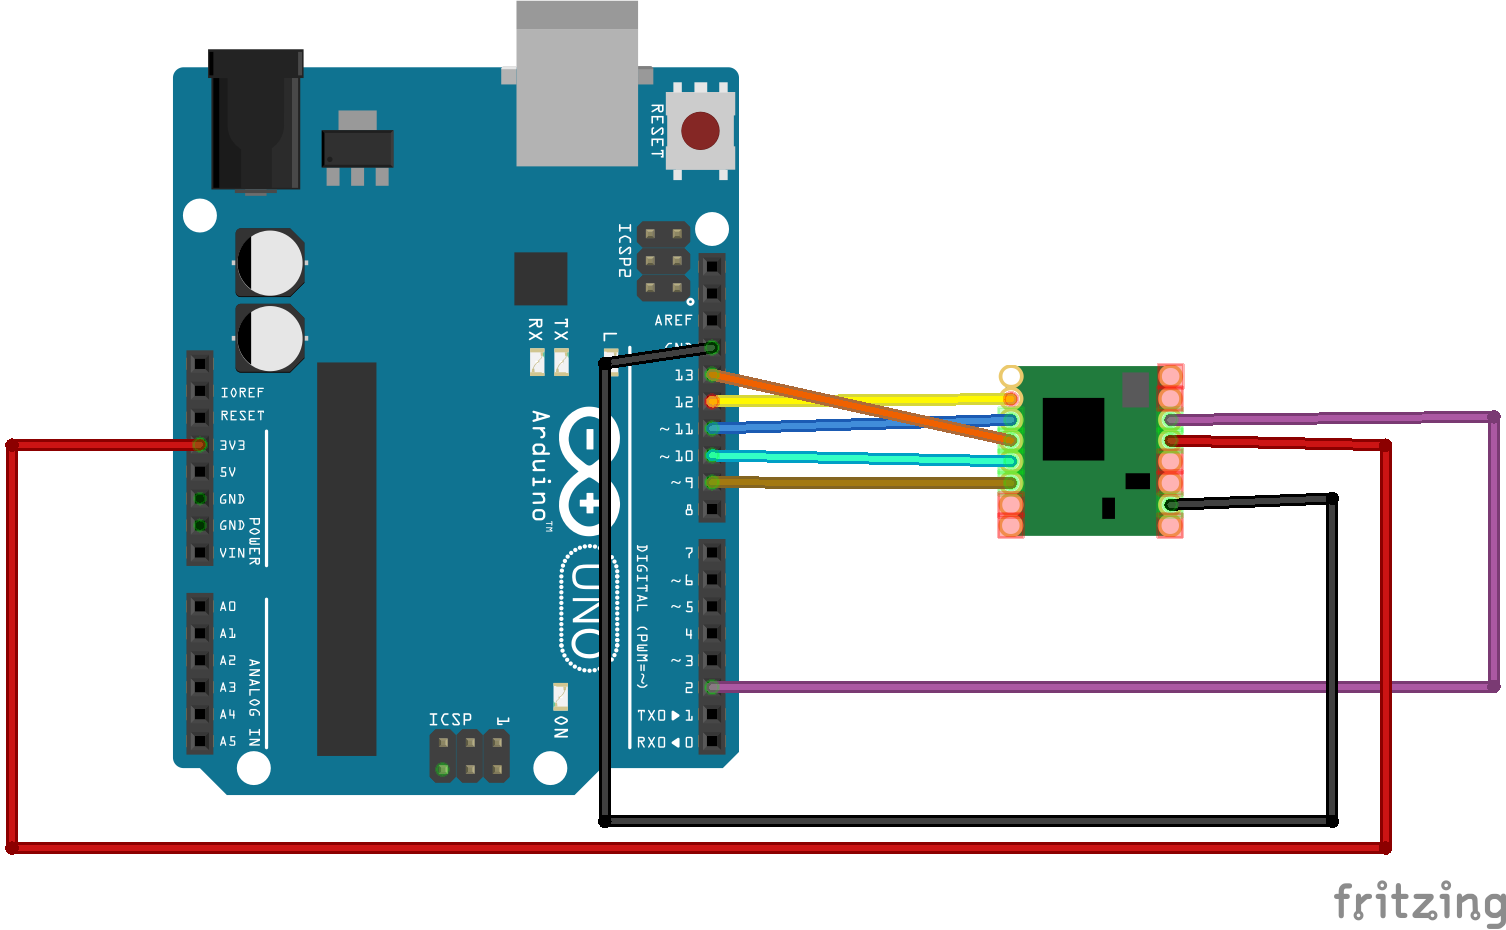
\includegraphics[width=0.75\textwidth]{unowire.png}
    \legend{Fonte: Autor}
    \label{fig:unowire}
\end{figure}


A imagem \ref{fig:esp32wire} representa a conexão feita entre o Heltec ESP32 LoRa e o sensor de temperatura DS18B20 compondo o outro dispositivo de borda.
\begin{figure}[ht]
    \centering
    \caption{Ligação entre DS18B20 e Heltec ESP32 LoRa}
    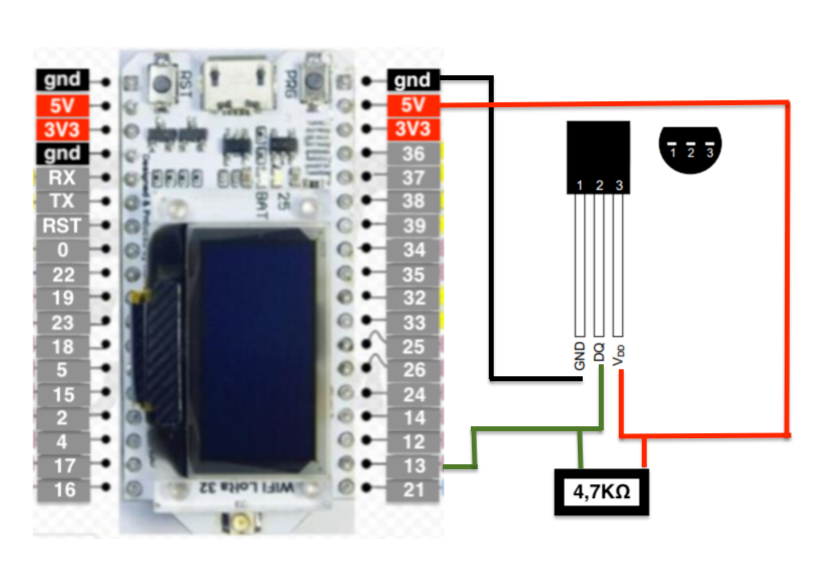
\includegraphics[width=0.75\textwidth]{esp32wire.png}
    \legend{Fonte: Autor}
    \label{fig:esp32wire}
\end{figure}

A imagem \ref{fig:rpiwire} representa a conexão feita entre o \textit{Raspberry Pi} e o  módulo RFM95W. O hardware resultante é o \textit{gateway} que recebe mensagem com comunicação LoRa.
\begin{figure}[ht]
    \centering
    \caption{Ligação entre RFM95W e \textit{Raspberry Pi}}
    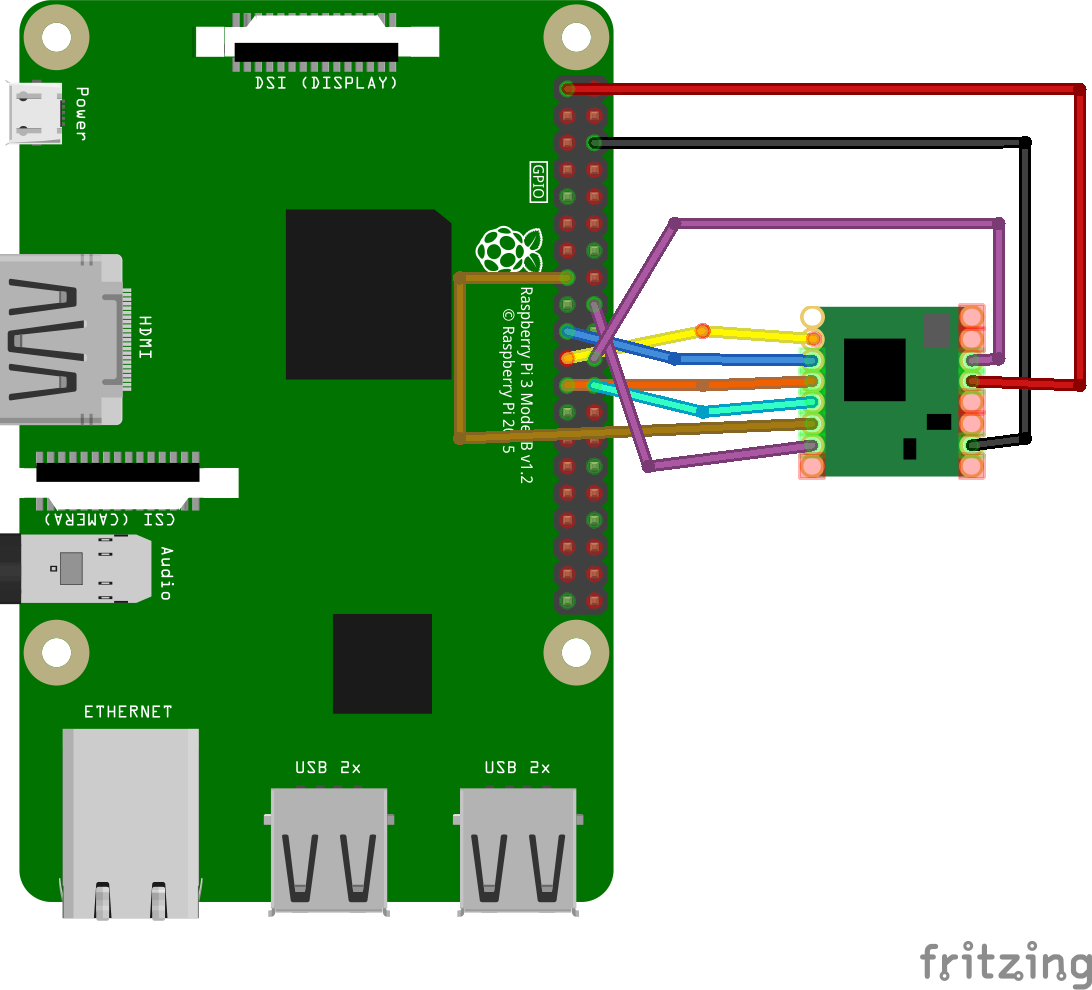
\includegraphics[width=0.75\textwidth]{rpiwire.png}
    \legend{Fonte: Autor}
    \label{fig:rpiwire}
\end{figure}

% ---
\chapter{Repositório de código e páginas sobre as tecnologias utilizadas} \label{anexosoftware}
% ---

\textbf{Biblioteca \textit{RadioHead} de comunicação com módulos RF}: 
\\
https://github.com/hallard/RadioHead

\textbf{SDK escrito em C para AWS IoT}: 
\\
https://github.com/aws/aws-iot-device-sdk-embedded-C

\textbf{SDK escrito em \textit{Python} para AWS IoT}:  
\\
https://github.com/aws/aws-iot-device-sdk-python

\textbf{SDK escrito em \textit{JavaScript} para AWS IoT}:  
\\
https://github.com/aws/aws-iot-device-sdk-js

\textbf{Repositório dos Códigos escritos para este trabalho de conclusão de curso}:
\\
https://github.com/pauloapanucci/lora

\textbf{Página do Polymer}: 
\\
https://www.polymer-project.org

% % ---
% \chapter{Fusce facilisis lacinia dui}
% % ---

% \lipsum[32]

\end{anexosenv}
%
%%---------------------------------------------------------------------
%% INDICE REMISSIVO
%%---------------------------------------------------------------------
%\phantompart
%\printindex
%%---------------------------------------------------------------------

\end{document}
